%% LaTeX2e class for student theses
%% thesis.tex
%% 
%% Karlsruhe Institute of Technology
%% Institute for Program Structures and Data Organization
%% Chair for Software Design and Quality (SDQ)
%%
%% Dr.-Ing. Erik Burger
%% burger@kit.edu
%%
%% Version 1.3.3, 2018-04-17

%% Available page modes: oneside, twoside
%% Available languages: english, ngerman
%% Available modes: draft, final (see README)
\documentclass[twoside, ngerman, draft]{sdqthesis}
\usepackage{todonotes}
%% ---------------------------------
%% | Information about the thesis  |
%% ---------------------------------

%% Name of the author
\author{Thomas Czogalik}

%% Title (and possibly subtitle) of the thesis
\title{Modellierung und Simulation von verteilter und wiederverwendbarer nachrichtenbasierter Middleware}

%% Type of the thesis 
\thesistype{Masterarbeit}

%% Change the institute here, ``IPD'' is default
% \myinstitute{Institute for \dots}

%% You can put a logo in the ``logos'' directory and include it here
%% instead of the SDQ logo
% \grouplogo{myfile}
%% Alternatively, you can disable the group logo
% \nogrouplogo

%% The reviewers are the professors that grade your thesis
\reviewerone{Prof. Dr.-Ing. Anne Koziolek}
\reviewertwo{Prof. Dr. Ralf H. Reussner}

%% The advisors are PhDs or Postdocs
\advisorone{M.Sc. Dominik Werle}
%% The second advisor can be omitted
\advisortwo{M.Sc. Stephan Seifermann}

%% Please enter the start end end time of your thesis
\editingtime{13. August 2018}{12. Februar 2019}

\settitle

%% --------------------------------
%% | Settings for word separation |
%% --------------------------------

%% Describe separation hints here.
%% For more details, see 
%% http://en.wikibooks.org/wiki/LaTeX/Text_Formatting#Hyphenation
\hyphenation{
% me-ta-mo-del
}

%% --------------------------------
%% | Bibliography                 |
%% --------------------------------

%% Use biber instead of BibTeX, see README
\usepackage[citestyle=numeric,style=alphabetic,backend=biber]{biblatex}
\usepackage{multirow}
\usepackage{tikz}
\usepackage{pgfgantt}
\usepackage{geometry} % to change margins
\usepackage{adjustbox}
\usepackage{listings}
\usepackage{pdflscape} % provides the landscape environment
\usepackage{ragged2e} % provides \RaggedLeft
\usetikzlibrary{shapes.geometric, arrows}

\addbibresource{thesis.bib}

%% ====================================
%% ====================================
%% ||                                ||
%% || Beginning of the main document ||
%% ||                                ||
%% ====================================
%% ====================================
\begin{document}

%% Set PDF metadata
\setpdf

%% Set the title
\maketitle

%% The Preamble begins here
\frontmatter

%% LaTeX2e class for student theses: Declaration of independent work
%% sections/declaration.tex
%% 
%% Karlsruhe Institute of Technology
%% Institute for Program Structures and Data Organization
%% Chair for Software Design and Quality (SDQ)
%%
%% Dr.-Ing. Erik Burger
%% burger@kit.edu
%%
%% Version 1.3.3, 2018-04-17

\thispagestyle{empty}
\null\vfill
\noindent\hbox to \textwidth{\hrulefill} 
\iflanguage{english}{I declare that I have developed and written the enclosed
thesis completely by myself, and have not used sources or means without
declaration in the text.}%
{Ich versichere wahrheitsgemäß, die Arbeit
selbstständig angefertigt, alle benutzten Hilfsmittel vollständig und genau
angegeben und alles kenntlich gemacht zu haben, was aus Arbeiten anderer
unverändert oder mit Änderungen entnommen wurde.}
 
 
%% ---------------------------------------------
%% | Replace PLACE and DATE with actual values |
%% ---------------------------------------------
\textbf{Karlsruhe, 12. Februar 2019}
\vspace{1.5cm}
 
\dotfill\hspace*{8.0cm}\\
\hspace*{2cm}(\theauthor) 
\cleardoublepage

\setcounter{page}{1}
\pagenumbering{roman}

%% ----------------
%% |   Abstract   |
%% ----------------
 
%% For theses written in English, an abstract both in English
%% and German is mandatory.
%%
%% For theses written in German, a German abstract is sufficient.
%%
%% The text is included from the following files:
%% - sections/abstract

\includeabstract

%% ------------------------
%% |   Table of Contents  |
%% ------------------------
\tableofcontents

\listoffigures
\listoftables

%% -----------------
%% |   Main part   |
%% -----------------

\mainmatter

%% LaTeX2e class for student theses
%% sections/content.tex
%% 
%% Karlsruhe Institute of Technology
%% Institute for Program Structures and Data Organization
%% Chair for Software Design and Quality (SDQ)
%%
%% Dr.-Ing. Erik Burger
%% burger@kit.edu
%% burger@kit.edu
%%
%% Version 1.3.3, 2018-04-17

\chapter{Einleitung}
\label{ch:Introduction}
Moderne Softwaresysteme werden über immer größere Entfernungen verteilt, laufen in unterschiedlichen Umgebungen, auf verschiedener Hardware und Betriebssystemen und sind noch dazu in verschiedenen Programmiersprachen geschrieben. Gleichzeitig werden hohe Anforderungen an Performance, Verfügbarkeit und Sicherheit gestellt. Dies führt dazu, dass auch die Anforderungen an ihre Kommunikationsinfrastruktur steigen. \par
Mithilfe von nachrichtenbasierter Middleware (MOM) lassen sich diese Anforderungen erfüllen. Ein Benutzer einer MOM kann sowohl Nachrichten empfangen, als auch senden. Dazu muss er nur mit der MOM verbunden sein. Er muss keine Informationen über die anderen Benutzer haben. Die MOM fügt eine Zwischenschicht zwischen den Sendern und Empfängern ein und ermöglicht dadurch Entkopplung und gleichzeitig einen asynchronen Nachrichtenaustausch, sodass die einzelnen Benutzer nicht blockieren müssen, wenn sie eine Nachricht senden oder empfangen wollen. Warteschlangen sind dabei ein wichtiger Bestandteil von MOMs. Sie dienen dem senden und empfangen von Nachrichten. Existierende Arbeiten vernachlässigen den Einfluss von Warteschlangen in Systemen mit einer MOM. Dadurch können bestimmte Effekte der MOM nicht abgebildet werden, wie zum Beispiel, dass die Zustellungsdauer im Zusammenhang mit dem Füllstand der Warteschlange steht.\par
\emph{ActiveMQ}, \emph{Kafka}, \emph{RabbitMQ}, \emph{Amazon MQ} oder \emph{ZeroMQ} sind nur ein paar Beispiele von MOMs. Es gibt eine Vielzahl von verschiedenen MOMs, die jeweils unterschiedliche Ziele oder Schwerpunkte haben. \emph{Kafka} legt zum Beispiel mehr Wert auf Performance als auf Verfügbarkeit \cite{kafka}, während \emph{RabbitMQ} eine allseitig einsetzbare MOM ist \cite{rabbitmq}. \par
%Um aus dieser Vielzahl an MOMs eine MOM für ein bestimmtes Softwaresystem auszuwählen ist bereits Expertenwissen notwendig. 
Neben der Vielzahl, an verschiedenen MOMs, bieten diese jeweils auch eine hohe Konfigurierbarkeit an, damit ein weiter Anwendungsbereich abgedeckt werden kann. Der jeweilige Benutzer kann auf spezielle Anforderungen seines Systems reagieren und die MOM dementsprechend anpassen. Eine mögliche Konfiguration könnte zum Beispiel dazu führen, dass die MOM weniger performant ist, aber dafür die Verfügbarkeit verbessert wird. Eine MOM so zu konfigurieren, dass sie den Wünschen des Benutzer entspricht, ist nicht trivial und benötigt Expertenwissen. 

\section{Ziel}
Das Ziel dieser Masterarbeit ist es, den Softwarearchitekten bei der Wahl einer MOM zu unterstützen. Die Unterstützung soll bereits in der Designphase stattfinden. Um dies zu ermöglichen, soll es für den Softwarearchitekten möglich sein einen wiederverwendbaren MOM-Modellbaustein auszuwählen und damit eine Softwarearchitektur, mithilfe einer Performance-Analyse, zu untersuchen. Somit ist bereits auf Modellebene die Auswirkung der Entscheidung zu sehen und der Architekt kann früh darauf reagieren. Um dies zu erreichen, soll im Rahmen dieser Masterarbeit eine Methode entwickelt werden, wie aus einer MOM ein wiederverwendbarer Modellbaustein wird, in dem Warteschlangen explizit modelliert sind. Dazu wird zunächst eine MOM mit einem Benchmark ausgemessen und im Anschluss modelliert. Mithilfe der Messergebnisse kann die Modellierung kalibriert werden, um im Anschluss eine Performance-Analyse zu ermöglichen. Außerdem wurde eine Modeltransformation konzipiert, um bereits existierende Modell-Elemente, zum Abbilden event-basierter-Kommunikation, wiederzuverwenden. Mithilfe eines Evaluierungssystem soll schließlich überprüft werden, ob mithilfe des Prozesses das Ziel der Masterarbeit erreicht werden konnte.

\section{Aufbau}
Im Folgenden wird der Aufbau der Masterarbeit beschrieben. In \autoref{ch:Grundlagen} werden Grundlagen erläutert, die für die weitere Arbeit benötigt werden. In \autoref{ch:Verwandte} wird ein Überblick über themenverwandte Arbeiten gegeben. Sie werden kurz zusammengefasst und diskutiert, in
wie weit sie für die Masterarbeit relevant sind, bzw. wie sich die Masterarbeit abgrenzt. \autoref{ch:mom} wählt eine konkrete MOM aus und untersucht sie. Die Modellierung einer MOM wird anschließend in \autoref{ch:modellierung} beschrieben. Um bestehende Elemente wiederverwenden zu können wird in \autoref{ch:transformation} eine Modelltransformation beschrieben. In \autoref{ch:Evaluation} wird die Modellierung mithilfe eines Fallbeispiels evaluiert. Schließlich wird in \autoref{ch:zusammenfassung} die Masterarbeit zusammengefasst und ein Ausblick für zukünftige Arbeiten gegeben.
%Wieso werden mqs verwendet? \\
%- entkoplung \\
%- skallierbarkeit (horizontal/vertikal) \\
%- async Kommunikation \\
%% batching (mehrere Eintraege auf einmal einfuegen)\\
%- wiederverwendbarkeit\\
%- arbeit aufteilen \\
%- bestimmte Garantien die MQ Liefert (reihenfolge, garantierte Lieferung) \\
%- lastspitzen puffern \\
%- gegen ausfaelle schutzen (Redundanzen) \\


%Problem: \\
%-	Keine Performanz Vorhersage für MQs \\
%-	Auswirkungen von Konfigurationen unbekannt \\
%Idee: wollen bei auswahl von MQ System unterstuetzen \\
%- sowohl bei der Plannung als auch in der Evolution des Systems \\
%- Nicht den Entwickler des MQ Systems, aber wie Würde das aussehen, wenn doch? (Abgrenzung) \\
%Vorteil:\\
%- MQ Abwaegung auf Architekturebene\\
%Aktion:\\
%- experiment \\
%%- modellierung \\
%- evaluierung 

%% LaTeX2e class for student theses
%% sections/content.tex
%% 
%% Karlsruhe Institute of Technology
%% Institute for Program Structures and Data Organization
%% Chair for Software Design and Quality (SDQ)
%%
%% Dr.-Ing. Erik Burger
%% burger@kit.edu
%% burger@kit.edu
%%
%% Version 1.3.3, 2018-04-17

\chapter{Grundlagen}
\label{ch:Grundlagen}
Dieses Kapitel beschreibt die in dieser Masterarbeit verwendete Terminologie und eine Übersicht über die Grundlagen auf der diese Masterarbeit aufbaut. Dazu wird zunächst die Domäne der nachrichtenbasierten Middleware (MOM) in \autoref{sec:mom} beschrieben. \autoref{sec:mdsd} beschreibt den Ansatz der modellgetriebenen Softwareentwicklung. In \autoref{sec:palladio} wird das Palladio-Komponentenmodell (PCM) vorgestellt, dass die Grundlage für die Implementierung dieser Masterarbeit zur Verfügung stellt.

\section{Nachrichtenbasierte Middleware (MOM)}
\label{sec:mom}
Event-basierte Systeme bestehen aus Events (Ereignis), Sendern, Empfängern und einer Middleware \cite{Carzaniga1998}. In einem solchen System werden Events von einem Sender instantiiert und von einem Empfänger entgegengenommen. Events sind dabei signifikante Änderungen eines Zustands \cite{Chandy2006}. Unter signifikant versteht man Änderungen, die das System beeinflussen. Dieser Transport von Events zwischen Sender und Empfänger wird durch die Middleware ermöglicht. Eine solche Middleware nennt man eine nachrichtenbasierte Middleware (MOM) \cite{Curry05}. Diese bietet eine Infrastruktur zum asynchronen Senden und Empfangen von Nachrichten, in verteilten Systemen an. Teilnehmer einer MOM müssen nicht blockieren und warten, wenn sie eine Nachricht senden oder empfangen wollen. Dieser asynchroner Mechanismus ist ein großer Vorteil. Außerdem führen MOMs eine Vermittlerschicht zwischen Sender und Empfänger ein, die für den Nachrichtenaustausch genutzt wird. Diese Zwischenschicht führt zu einer losen Kopplung der einzelnen Komponenten.  \\
%- Vorteile \\
%- Standards \\
%-- wie jms and amqp \\

\subsection{Architektur}
MOMs unterscheiden sich, neben ihrer Implementierung, in ihrer Architektur. Es gibt drei verschiedene Architekturen für MOMs \cite{Rathfelder2013}:
\begin{itemize}
\item Die \textbf{Peer-To-Peer} Architektur, hat keinen ausgewählten Knoten, der die MOM bereitstellt. Die Funktionalität, die zum Kommunizieren benötigt wird, wird von den Sendern und Empfängern bereitgestellt.
\item In der \textbf{zentralen} Variante läuft die MOM auf einem zentralen Knoten. Alle Sender und Empfänger sind mit diesem Knoten verbunden. 
\item Schließlich gibt es noch die \textbf{verteilte} Architektur. Die MOM ist über mehrere Knoten verteilt. Der Austausch von Daten wird mithilfe von Routing-Algorithmen bewerkstelligen. Sender und Empfänger müssen nicht mit dem selben Middlewareknoten verbunden sein.
\end{itemize}  

\subsection{Warteschlangen}
Warteschlangen sind ein wichtiger Bestandteil von MOMs \cite{Curry05}, vor allem für deren asynchronen Nachrichtenaustausch. Sender nutzen sie um Nachrichten abzulegen. Empfänger nutzen sie um Nachrichten abzuholen. Die Nachrichten in der Warteschlange sind nach einer festgelegten Ordnung geordnet, z.B. First-In-First-Out, also die Nachricht, die als erstes in die Warteschlange eingefügt wurde, wird auch als erste wieder herausgenommen. Eine Warteschlange kann i.d.R. von einem Nutzer konfiguriert werden. Mögliche Konfigurationen für eine Warteschlange können Größe, Verweildauer oder Sortierung sein.

\subsection{Nachrichtenmodelle}
\label{sec:nachrichtenmodelle}
Wie eine MOM Nachrichten austauscht, wird in ihrem Nachrichtenmodell festgelegt. Man unterscheidet dabei zwischen dem Point-To-Point und dem Publish/Subscribe Modell \cite{Curry05}. Eine MOM kann auch aus einer Kombination der beiden Modelle bestehen um auf bestimmte Szenarien reagieren zu können.
\begin{itemize}
\item Im \textbf{Point-To-Point} Modell werden Nachrichten von einem Sender an eine bestimmte  Warteschlange gesendet. Normalerweise ist eine Warteschlange mit genau einem Empfänger verbunden. Es können aber auch mehrere Empfänger mit einer Warteschlange verbunden sein. Die Nachrichten werden in diesem Fall nach dem First-Come-First-Serve (FCFS) Prinzip entnommen und verarbeitet. 
\item Beim \textbf{Publish/Subscriber} Modell verbindet sich der Empfänger (Subscriber) mit der MOM und legt, für die Nachrichten die er Empfangen möchte, Bedingungen fest \cite{Eugster03}. Dabei wird zwischen drei Arten von Bedingungen unterschieden \cite{Rathfelder2013}:
\begin{itemize}
    \item \textbf{Inhaltsbasiert}: Dabei lassen sich Filterregeln definieren, die auf den Inhalt und die Payload der Nachrichten angewendet werden können.
    \item \textbf{Kanalbasiert}: Die MOM bietet verschiedene Kanäle (Channel) an, an die Nachrichten gesendet werden können. Empfänger können sich an einem Kanal anmelden und erhalten alle Nachrichten, die an diesen Kanal gesendet werden.
    \item \textbf{Typbasiert}: Die Nachrichten werden anhand ihres Typs identifiziert und an die Empfänger weitergeleitet.
\end{itemize}
\end{itemize}

\subsection{Interaktionstypen}
Der Interaktionstyp einer MOM gibt an, wie viele Sender und Empfänger an einer Kommunikation teilnehmen können. Dabei wird zwischen den folgenden Typen unterschieden \cite{Rathfelder2013}:
\begin{itemize}
    \item \textbf{Eins-Zu-Eins}: Genau ein Sender und ein Empfänger können an einer Interaktion teilnehmen.
    \item \textbf{Eins-Zu-Vielen}: Es gibt einen Sender und mehrere Empfänger, die an einer Interaktion teilnehmen können. 
    \item \textbf{Viele-Zu-Eins}: Mehrere Sender senden an einen Empfänger.
    \item \textbf{Viele-Zu-Viele}: Mehrere Sender und mehrere Empfänger nehmen an der Interaktion teil.
\end{itemize}

\subsection{Grad der Entkopplung}
Entkopplung der Komponenten ist ein Vorteil der durch nachrichtenbasierte Middleware versprochen wird. Dabei wird zwischen drei Aspekten der Entkopplung \cite{Eugster03} unterschieden:
\begin{itemize}
    \item \textbf{Synchronisation}: Die Kontrollflüsse, von Sender und Empfänger, sind entkoppelt. D.h. die Sender und Empfänger warten nicht aufeinander, sondern senden und empfangen asynchron Nachrichten.
    \item \textbf{Raum}: Sender wissen nicht mit wie vielen Empfängern sie kommunizieren und umgekehrt wissen die Empfänger nicht, wie viele Sender Nachrichten senden.
    \item \textbf{Zeit}: Sender und Empfänger müssen nicht gleichzeitig aktiv sein.
\end{itemize}

\section{Java Message Service (JMS)}
Der Java Message Service (JMS) ist eine standardisierte Programmierschnittstelle (API) \cite{jmsspec}. Sie dient dazu Java-Applikationen Zugriff auf nachrichtenbasierten Middlewares zu geben. Im JMS-Umfeld wird die MOM als JMS-Server und die Applikationen die die API verwenden, um Nachrichten auszutauschen, als JMS-Klienten bezeichnet. JMS ist Teil der \emph{Java Platform Enterprise Edition}, die Standards für Enterprise-Applikationen definiert. JMS unterstützt verschiedene Nachrichtentypen, wie Text-, Byte- oder Objektnachrichten. Es werden die beiden oben vorgestellten Nachrichtenmodelle, Punkt-Zu-Punkt und Publish/Subscriber Modell unterstützt. JMS unterscheidet zwischen persistenter und nicht-persistenter Nachrichtenzustellung. Im nicht-\\persistenten-Modus, werden Nachrichten in den Hauptspeicher geschrieben. Eine Nachricht wird außerdem auf die Festplatte geschrieben, wenn der Hauptspeicher voll ist. Nachrichten die im nicht-persistenten-Modus gesendet werden, werden maximal einmal ausgeliefert. Der persistente-Modus schreibt ankommende Nachrichten auf die Festplatte und in den Hauptspeicher. Außerdem wird garantiert, dass die Nachricht genau einmal ausgeliefert wird. 
Die API wird bei der Untersuchung der MOM und bei der Evaluierung benötigt.

\section{Modellgetriebene Softwareentwicklung}
\label{sec:mdsd}
In der modellgetriebenen Software-Entwicklung werden Teile des Software-Systems innerhalb von Modellen unter Nutzung von Abstraktionen beschrieben \cite{MDSD}. Das Ziel der modellgetriebenen Softwareentwicklung ist die Verbesserung der Softwarequalität und der Wiederverwendbarkeit. Modelle sind Entwicklungsartefakte und Systembestandteile. Außerdem erlauben sie das automatische Ableiten von Systemartefakten. Außerdem soll eine Erhöhung der Entwicklungseffizienz, zum Beispiel durch Quellcodeerzeugung, aus den Modellen erreicht werden.

\subsection{Modell}
Nach Herbert Stachowiak \cite{Stachowiak1973} zeichnet sich ein Modell durch die folgenden drei Merkmale aus.
\begin{itemize}
\item \textbf{Abbildung} - Bei einem Modell handelt es sich um eine Abbildung oder Repräsentation von einem künstlichen oder natürlichen Original. Das Original kann selbst wieder ein Modell sein. 
\item \textbf{Verkürzung} - Es werden nicht alle Attribute des Originals erfasst, sondern nur diejenigen, die relevant sind.
\item \textbf{Pragmatismus} - Modelle erfüllen ihre Ersatzfunktion für bestimmte Subjekte, innerhalb einer bestimmten Zeit und unter Einschränkung bestimmter gedanklicher oder tätlicher Operationen. Beispielsweise benötigt eine Analyse je nach gewünschter Genauigkeit, unterschiedlich genaue Modelle. Der Pragmatismus schreibt vor, dass man hier nicht unnötig genau arbeitet.
\end{itemize} 
\subsection{Meta-Modell}
Ein Meta-Modell beschreibt die Struktur eines Modells. Dabei muss ein Meta-Modell die folgenden Bereiche abdecken:
\begin{itemize}
\item \textbf{Abstrakte Syntax}: Sie beschreibt die Konstrukte, aus denen die Modelle bestehen, sowie deren Eigenschaften und Beziehungen.
\item \textbf{Konkrete Syntax}: Diese beschreibt die Darstellung der Konstrukte, Eigenschaften und Beziehungen, die in der abstrakten Syntax spezifiziert sind.
\item \textbf{Statische Semantik}: Mithilfe dieser werden Modellierungsregeln und Einschränkungen ausgedrückt, die mit der abstrakten Syntax nicht möglich sind.
\item \textbf{Dynamische Semantik}: Sie drückt die Bedeutung der Konstrukte aus und wird oft nicht formal, sondern durch natürlich sprachlichen Text spezifiziert.
\end{itemize}

\subsection{Modeltransformation}
Bei der Modelltransformation \cite{Kleppe03} wird ein Quellmodell in ein Zielmodell übersetzt. Dies geschieht mithilfe einer Transformationsdefinition. Die Transformationsdefinition besteht aus einer Menge von Transformationsregeln, die beschreiben wie ein Modell in ein anderes überführt wird. Dabei wird zwischen zwei Arten der Modelltransformation unterschieden:
\begin{itemize}
    \item \textbf{Modell-Zu-Modell}: Dabei wird ein Quellmodell, dass zu einem Quellmetamodell konform ist, in ein Zielmodell, dass zu einem Zielmetamodell konform ist, transformiert.
    \item \textbf{Modell-Zu-Text}: Dabei wird ein Modell in eine oder mehrere Textdateien übersetzt. Meistens beinhalten diese Quellcode einer gegebenen Programmiersprache. Eine Transformation kann aber auch Dokumentation oder Konfigurationen generieren.
\end{itemize}
Für die Masterarbeit wurde eine Modell-Zu-Modell Transformation beschrieben/entwickelt.
\section{Palladio Komponenten Modell}
\label{sec:palladio}
Das Palladio Komponentenmodell (PCM) \cite{palladio17} ist eine Architecture-Description-Language (ADL) und unterstützt die Erstellung skalierbarer, zuverlässiger, wartbarer und wiederverwendbarer komponenentenbasierter Softwarearchitekturen. Eine Komponente ist ein vertraglich festgelegter Baustein, der zusammengestellt, eingesetzt und angepasst werden kann, ohne seine Interna zu kennen. Neben der Beschreibung von Softwarearchitekturen, sind auch Qualitätsanalysen, bezüglich der Performance, Zuverlässigkeit und Kostenschätzung möglich. Im Folgenden werden Teile des PCM erklärt, die für die Masterarbeit benötigt werden.

%\subsection{Viewpoints}
%- structural (assembly) \\
%- behaviour (sequence?) \\
%- deployment (allocation, deployment decision) \\
\subsection{Rollen}
%s.203
Die Modellierung der verschiedenen MOMs erfolgt mithilfe von Software-Architektur-Modellen. In der modellgetriebenen Softwareentwicklung und in Palladio gibt es dabei verschiedene Rollen, die an unterschiedlichen Teilen der Architektur arbeiten und dort ihr spezifisches Wissen einbringen.
\begin{itemize}
\item Die Architektur und der Zusammenhang der einzelnen Komponenten
miteinander werden vom \textbf{Softwarearchitekt} entworfen. Er ist auch dafür
zuständig weitere Anweisungen an die anderen Rollen weiterzugeben. Gleichzeitig ist er für das \textbf{System-Modell} zuständig, das die Zusammensetzung der Komponenten charakterisiert.
\item Das Wissen darüber, wie der Benutzer mit dem System interagiert
und welche Parameter im Kontrollfluss verwendet werden, stammt vom \textbf{Domänenxperten}. Die Modellierung wird im \textbf{Usage-Modell} festgehalten.
\item Für das Implementieren und Spezifizieren der einzelnen
Komponenten ist der \textbf{Komponentenentwickler} verantwortlich. Diese modelliert er im \textbf{Repository-Modell}. Es enthält die einzelnen Komponenten und Schnittstellen.
\item Die Zusammenstellung der Systemumgebung der Software wird vom \textbf{Softwareverteilungsexperten} übernommen. Diese wird von ihm im \textbf{Ausführungsum-gebungs-Modell} festgehalten. Außerdem weist der Softwareverteilungsexperte den Komponenten Ressourcen zu. Dies hält er im \textbf{Komponenten-Allokations-Modell} fest.
\end{itemize}
Die Modelle, die von den verschiedenen Rollen entwickelt und gewartet werden, bilden zusammen eine Palladio-Modellinstanz. Mithilfe der Modellierung einer MOM sollen die verschiedenen Rollen unterstützt werden. 

\subsection{Teilmodelle}
Wie bereits erwähnt, sind die einzelnen Rollen für bestimmte Teilmodelle zuständig, die zusammen die vollständige Architekturbeschreibung ergeben. Im Folgenden sollen die Teilmodelle des PCM genauer beschrieben werden.
\subsubsection{Repository-Modell (Component-Repository-Model)} 
Das Repository-Modell enthält Datentypen, Schnittstellen und Komponenten. Eine Komponente kann ihre Funktionalität über eine Schnittstelle nach außen anbieten. Dies wird mit einer \emph{ProvidedRole} modelliert. Sie kann außerdem fordern, dass eine bestimmte Schnittstelle verfügbar sein muss, damit sie ihre Funktionalität anbieten kann. Dies wird mit einer \emph{RequiredRole} modelliert. Schnittstellen enthalten eine Sammlung an Signaturen, die eine Operation repräsentieren. 
%In (ABB) ist ein Beispiel für ein Repository-Modell. Darin sind eine ISupermarkt- und IZulieferer-Schnittstelle abgebildet. Außerdem eine Supermarkt- und Zulieferer-Komponente. Die Supermarkt-Komponenten bietet ihre Funktionalität über die ISupermarkt-Schnittstelle an.  Die Schnittstelle enthält eine Signatur für eine Operation verkaufen(String warenName). Außerdem benötigt die Supermarkt-Komponente eine Komponente, die IZulieferer anbietet. Dies wird mit einer RequiredRole modelliert. Die Zulieferer-Komponente bietet ihre Funktionalität über die IZulieferer-Schnittstelle an. 
Mithilfe einer Service-Effect-Specification (SEFF) kann das Verhalten innerhalb der Komponenten beschrieben werden. Das Verhalten kann mit einer \emph{InternalCallAction} und einer \emph{ExternalCallAction} modelliert werden. Eine \emph{InternalCallAction} repräsentiert einen Aufruf zu Code, der sich innerhalb der Komponente befindet. Eine \emph{ExternalCallAction} ruft eine Operation in einer anderen Komponente auf. Mithilfe einer \emph{UsageVariable} kann eine Parameterbelegung für den Aufruf spezifiziert werden. Außerdem lassen sich im SEFF Ressourcenanforderungen an bestimmte Ressourcen, wie zum Beispiel CPU,  spezifizieren. Die Ressourcenanforderungen werden dabei als abstrakte Arbeitspakete angegeben. Wenn eine konkrete Ausführungsumgebung vorliegt, in der die Ressourcen spezifiziert sind, lassen sich Zeitwerte aus den abstrakten Arbeitspaketen ableiten. Durch Angabe eines SEFFs kann das Modell analysiert werden.
%In dem Beispiel ist ein SEFF in der Supermarkt-Komponente, der das Verhalten für die Operation ISupermarkt.verkaufen abbildet.  Der Kontrollfluss beginnt mit dem Ausführen der InternalAction \textbf{prüfeVorätig}. Eine InternalAction repräsentiert dabei einen Aufruf zu Code, der sich innerhalb der Komponente befindet. Außerdem können damit Ressourcen angefordert werden. Im Beispiel werden CPU-Einheiten angefordert. Im Anschluss wird mit einer ExternalCallAction eine Operation in einer anderen Komponente, hier IZulieferer.liefere aufgerufen, wenn weniger als zehn Waren vorrätig sind. 
Verzweigungen können mit einer \emph{BranchAction} modelliert werden. Dabei kann entweder eine Wahrscheinlichkeit oder eine Bedingung angegeben werden, welche Verzweigung genommen wird. 
%Der Software-Architekt verwendet es um Komponenten zu entnehmen und neue Schnittstellen zu spezifizieren. Der Komponentenentwickler nutzt es um neue Komponenten zu erstellen und darin abzulegen. 
\subsubsection{Systemmodell (System-Model)}
Das Systemmodell repräsentiert das Software-System, das aus einer Zusammensetzung der im Repository-Modell definierten Komponenten besteht. Mithilfe von einem \emph{AssemblyContext} werden Instanzen von Komponenten im Systemmodell dargestellt. Diese können mit einem \emph{AssemblyConnector} verbunden werden. Dabei wird die \emph{RequiredRole} einer Komponente mit der \emph{ProvidedRole} einer Komponente verbunden. Das Systemmodell muss außerdem mindestens eine Schnittstelle nach außen bereitstellen, damit mit dem System interagiert werden kann. 
%In (abb) ist ein Systemmodell für das bereits beschriebene Repository-Modell abgebildet. Darin sind drei Instanzen der Supermarkt-Komponente mit einer Instanz der Zulieferer-Komponente über jeweils einen AssemblyConnector verbunden. Außerdem bietet jede Instanz der Supermarkt-Komponente ihre Schnittstelle über die Systemgrenze hinaus an.
\subsubsection{Ausführungs-Umgebungs-Modell (Execution-Environmet-Model)}
Das Ausführungs-Umgebungs-Modell beschreibt die benutzte Hardware und das Netzwerk des modellierten Software-Systems. Dabei werden \emph{ResourceContainer} und \emph{LinkingResourceContainer} verwendet. Bei einem \emph{ResourceContainer} handelt es sich um eine Hardware-Ressource, bei einer \emph{LinkingResource} um einen Verbindungskanal zwischen zwei \emph{ResourceContainer}. Für einen \emph{ResourceContainer} lassen sich verschiedenen Hardware-Ressourcen angeben. Mit \emph{CPU} lässt sich ein Prozessor, mit \emph{HDD} eine Festplatte und mit \emph{Delay} eine Verzögerung zwischen zwei Aktionen modellieren.
%In (abb) sind außerdem die Elemente aus dem Ausführungs-Umgebungs-Modell abgebildet. In dem Beispiel wird sind zwei RessourceContainer mit dem Namen Supermärkte und Zulieferer abgebildet. Beide haben eine CPU und HDD Ressource. Außerdem werden sie mithilfe einer LinkingRessource verbunden.
\subsubsection{Allokations-Modell (Component-Allocation-Model)}
Das Allokations-Modell beschreibt wie die einzelnen Komponenteninstanzen auf der, im Ausführungs-Umgebungs-Modell beschriebenen, Hardware verteilt werden. Dazu wird ein \emph{AllocationContext} verwendet. 
%In (abb) werden die Komponenten-Instanzen des Beispiels auf jeweils einem RessourceContainer bereitgestellt. 
\subsubsection{Nutzungsmodell (Usage-Model)}
Das Nutzungsmodell beschreibt die Interaktion des Benutzers, oder eines externen Systems, mit dem System. Mit einem \emph{UsageScenario} kann das Verhalten eines Benutzers spezifiziert werden. Für ein \emph{UsageScenario} wird zunächst eine Arbeitslast (\emph{Workload}) festgelegt. Dabei unterscheidet man zwischen einem \emph{Open-} oder \emph{ClosedWorkload}. Ein \emph{OpenWorkload} modelliert einen unendlichen Strom an Benutzern die in festgelegten Zeitabständen (\emph{ArrivalTime}) am System ankommen und das Szenario ausführen. Ein \emph{ClosedWorkload} modelliert, dass eine feste Anzahl von Benutzern (\emph{Population}) das Szenario ausführt, dann  wartet (\emph{ThinkTime}) und dann wieder das Szenario ausführt. Ein Szenario kann mithilfe von einem \emph{EntryLevelSystemCall} eine vom System bereitgestellte Operation aufrufen. Dabei kann auch eine Parameterbelegung mithilfe einer \emph{UsageVariable} spezifiziert werden. 
%In (abb) ist eine UsageScenario abgebildet. Dabei wird ein OpenWorkload verwendet und 
\subsection{Qualitätsattribute}
Palladio kann Qualitätsattribute für ein System bestimmen, diese berechnet es aus den Komponenten, ihren Verbindungen und der Ausführungsumgebung. Der Fokus liegt dabei auf den folgenden Qualitätsattributen. 
\subsubsection{Performance} 
%(Buch S. 93/94)
Performance ist bezüglich des Zeitverhaltens eines Systems eines der wichtigsten Qualitätskriterien. Dies gilt sowohl für zeitkritische, als auch für weniger kritische Systeme. Performance beinhaltet das Zeitverhalten und die Ressourcen Nutzung eines Systems. Dies wird mit den folgenden drei Metriken gemessen:
\begin{itemize}
\item Die \textbf{Antwortzeit} ist die Zeit, die zwischen einer Anfrage an ein System und einer erhaltenen Antwort vergeht. Ein Beispiel hierfür kann die Anfrage an eine Suchmaschine sein, die nach einer Sekunde eine Antwort liefert.
\item Der \textbf{Durchsatz} bezeichnet die Menge an Anfragen, die pro Zeiteinheit verarbeitet werden können. Zum Beispiel kann ein Webserver 100 Anfragen pro Sekunde verarbeiten.
\item Die \textbf{Auslastung} bezieht sich auf die aktive Nutzung einer Ressource und gibt in Prozent an wie viel diese pro Zeiteinheit arbeitet. 
\end{itemize}
Mithilfe der Performance soll im Rahmen der Masterarbeit untersucht werden, wie sich diese auf das Gesamtsystem auswirkt, wenn verschiedene MOMs verwendet werden.
%- Abgrenzung zu dynamischen performanz parameter änderungen \\

\subsubsection{Zuverlässigkeit}
Ein System, das einen Dienst wie erwartet und ohne Seiteneffekte anbietet, wird als zuverlässig bezeichnet. Jede Abweichung vom erwarteten Verhalten wird als Fehler betrachtet. Die gesamt Zuverlässigkeit eines Systems wird deshalb als Wahrscheinlichkeit, dass das System fehlerfrei arbeitet, angegeben. Dabei können verschiedene Fehler auftreten:
\begin{itemize}
\item \textbf{Softwarefehler} können auftreten, aufgrund von Fehlern in der Implementierung.
\item \textbf{Hardwarefehler} können auftreten, weil bestimmte Ressourcen nicht verfügbar sind und somit ein Fehler in der Programmausführung auftritt.
\item \textbf{Netzwerkfehler} können aufgrund von verlorenen Nachrichten auftreten, die über das Netzwerk gesendet werden.
\end{itemize}
In Palladio ist es möglich Fehlerwahrscheinlichkeiten an Komponenten und Ressourcen zu annotieren. Dieses Qualitätsattribut ist auch für \gls{mom}s interessant, um zum Beispiel Auslieferungsgarantien oder den Ausfall einzelner Knoten zu betrachten. Im Rahmen der Masterarbeit wird dieses Qualitätsattribut nicht betrachtet.

\subsubsection{Kosten}
Hohe Anforderungen führen meist zu hohen Kosten. Deshalb muss i.d.R. zwischen Kosten und Performance oder Verlässlichkeit abgewogen werden. Palladio ermöglicht Kosten an Komponenten und Ressourcen zu annotieren um Gesamtkosten abzuschätzen und eine Abwägung zwischen den Qualitätsattributen zu treffen. Im Rahmen der Masterarbeit wird dieses Qualitätsattribut nicht betrachtet.

\subsection{Event-basierte Kommunikation im PCM}
%(Konzept erklären und nicht genaue Elemente des MM) \\
%Disertation s.103
In der Arbeit \cite{Rathfelder2013} wurden Events als Elemente erster Klasse in PCM eingeführt. Im Folgenden sollen Events in PCM vorgestellt werden, da diese im späteren Verlauf der Masterarbeit wiederverwendet werden sollen. \par
In event-basierten Systemen wird die Geschäftslogik in einer sogenannten Event-Handler-Methode implementiert und ausgeführt, wenn ein bestimmtes Event beim Empfänger ankommt. Der Sender und Empfänger müssen das jeweilige Event unterstützen, damit sie damit kommunizieren können. In komponentenbasierten Systemen werden solche Anforderungen mithilfe von Schnittstellen, die einen Vertrag zwischen den Kommunizierenden darstellt, umgesetzt. In event-basierten System besteht ein solcher Vertrag nicht aus Funktionen, sondern aus Events, die gesendet und empfangen werden können. In PCM wurde dazu eine \emph{EventGroup} eingeführt. Diese verhält sich ähnlich wie eine Schnittstelle. Eine \emph{EventGroup} spezifiziert anstatt einer Signatur, einen oder mehrere \emph{EventType}s. Ein \emph{EventType} kann dabei einen Payload haben. Eine Komponente die Events aus einer \emph{EventGroup} sendet, benötigt einen \emph{SourcePort}. Die Komponente die Events einer \emph{EventGroup} empfängt hat dagegen einen \emph{SinkPort}. Diese beiden Elemente verhalten sich ähnlich zu einer \emph{RequiredRole} und \emph{ProvidedRole}. 
Damit Komponenten Events senden und empfangen können werden Elemente benötigt, die das Senden und Empfangen ermöglichen. Der Sender kann mit einer \emph{EmitEventAction} innerhalb eines SEFF einen \emph{EventType} über den \emph{SourcePort} senden. Auf Empfänger Seite wird neben einem \emph{SourcePort} auch ein SEFF, der als Event-Handler dient, benötigt. In \autoref{img:grundlageneventsrepo} ist ein Beispiel Repository-Modell abgebildet. Darin sendet die Supermarkt-Komponente Nachrichten vom \emph{EventType} \emph{Bestellung} über ihren \emph{SourcePort}. Die Zulieferer-Komponente empfängt Nachrichten vom \emph{EventType} \emph{Bestellung} über ihren \emph{SinkPort}.

\begin{figure}
\center
  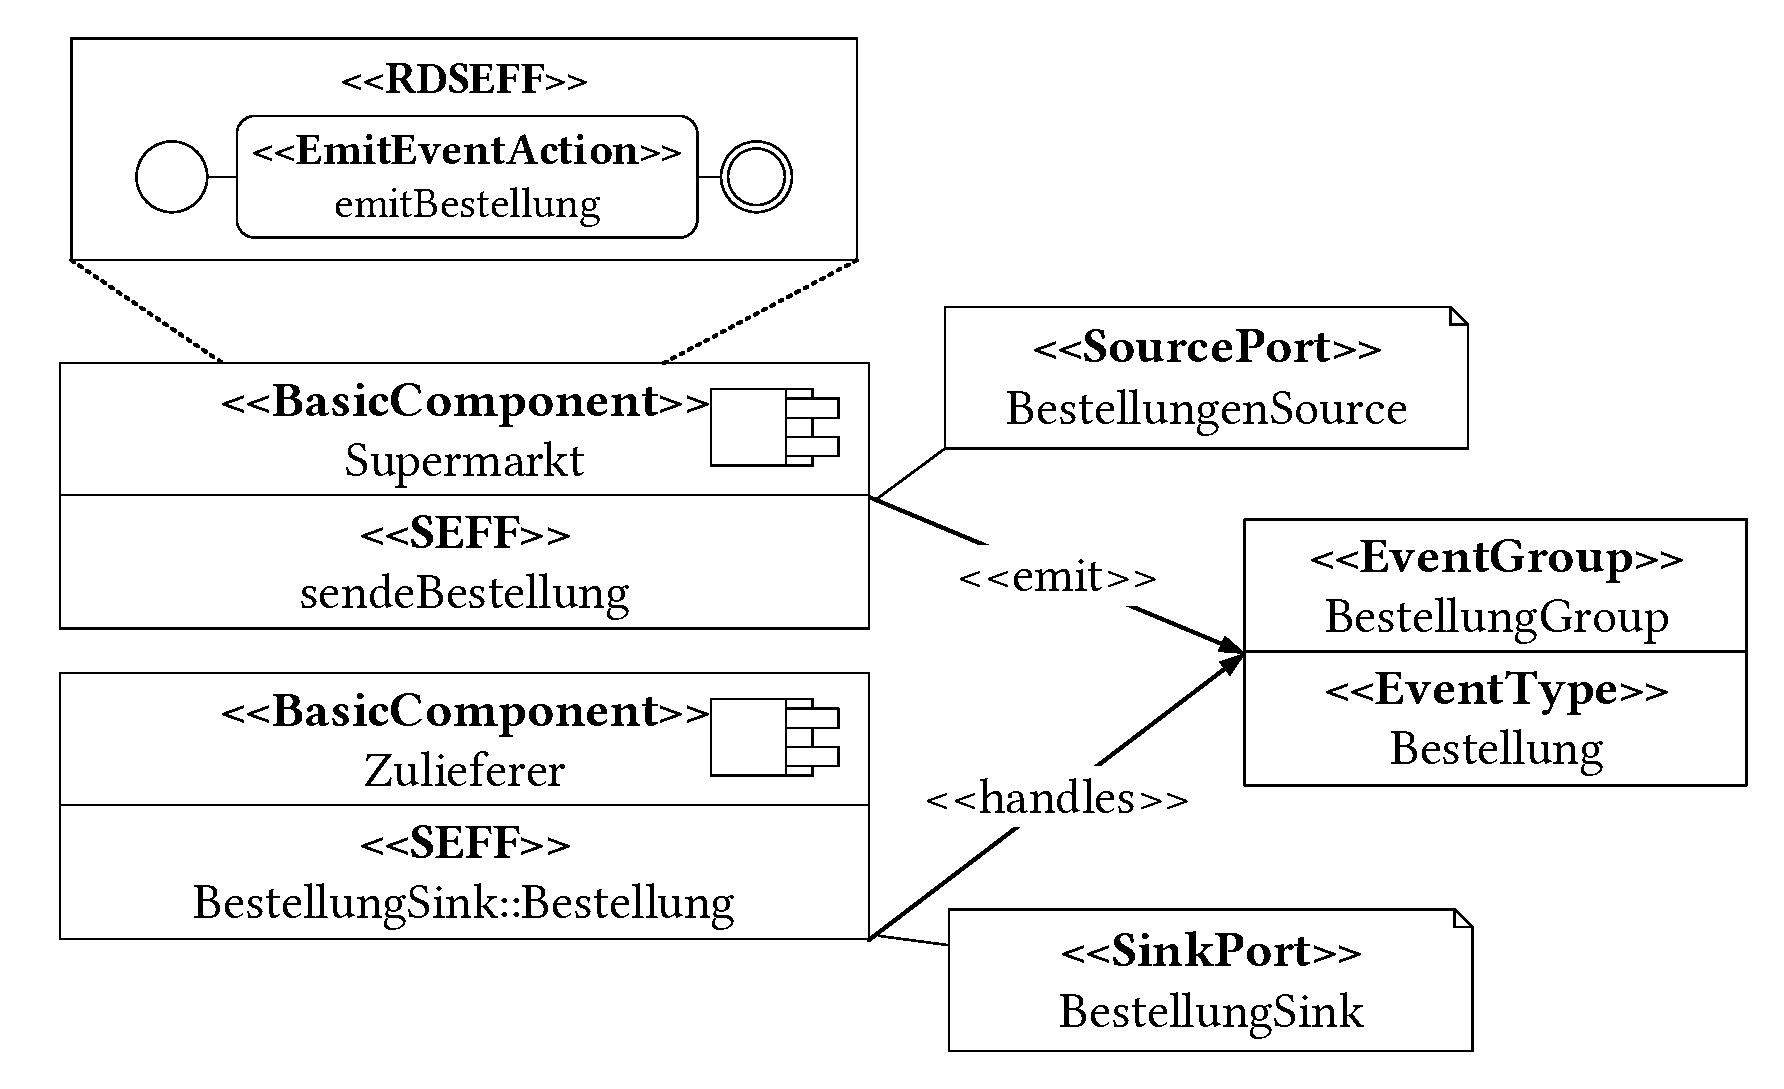
\includegraphics[width=1\textwidth]{images/grundlagen/grundlagenEventRepo.pdf}
  \caption{Repository-Modell mit Events.}
  \label{img:grundlageneventsrepo}
\end{figure}

Schließlich müssen die Komponenten im Systemmodell verbunden werden. Komponenten die Events senden und empfangen, werden über ihren \emph{SinkPort} und \emph{SourcePort} verbunden. Das PCM bietet dazu zwei Möglichkeiten und deckt damit die Nachrichtenmodelle aus \autoref{sec:nachrichtenmodelle} ab. Wenn Events direkt an eine Komponente geschickt werden sollen, werden die beiden Komponenten mithilfe eines \emph{P2PConnector} verbunden. Sollen Komponenten in einem Publish/Subscribe-Szenario miteinander kommunizieren, wird ein \emph{EventChannel} benötigt. Ein \emph{EventChannel} enthält genau eine \emph{EventGroup}. Die sendende Komponente verbindet ihren \emph{SourcePort} mit dem \emph{EventChannel}. Die empfangende Komponente verbindet ihren \emph{SinkPort} mit dem \emph{EventChannel}. In \autoref{img:grundlageneventssystem} sind zwei Systemmodelle abgebildet. Das erste zeigt eine Punkt-Zu-Punkt Verbindung zwischen einer Supermarkt- und Zulieferer-Komponente. Dabei sind der \emph{SourcePort} und der \emph{SinkPort} direkt mit einem \emph{P2PConnector} verbunden. Das zweite Systemmodell zeigt eine Publish/Subscribe Kommunikation zwischen mehreren Supermarkt-Komponenten und mehreren Zulieferer-Komponenten. Dabei wird über einen \emph{EventChannel} kommuniziert.

\begin{figure}
\center
  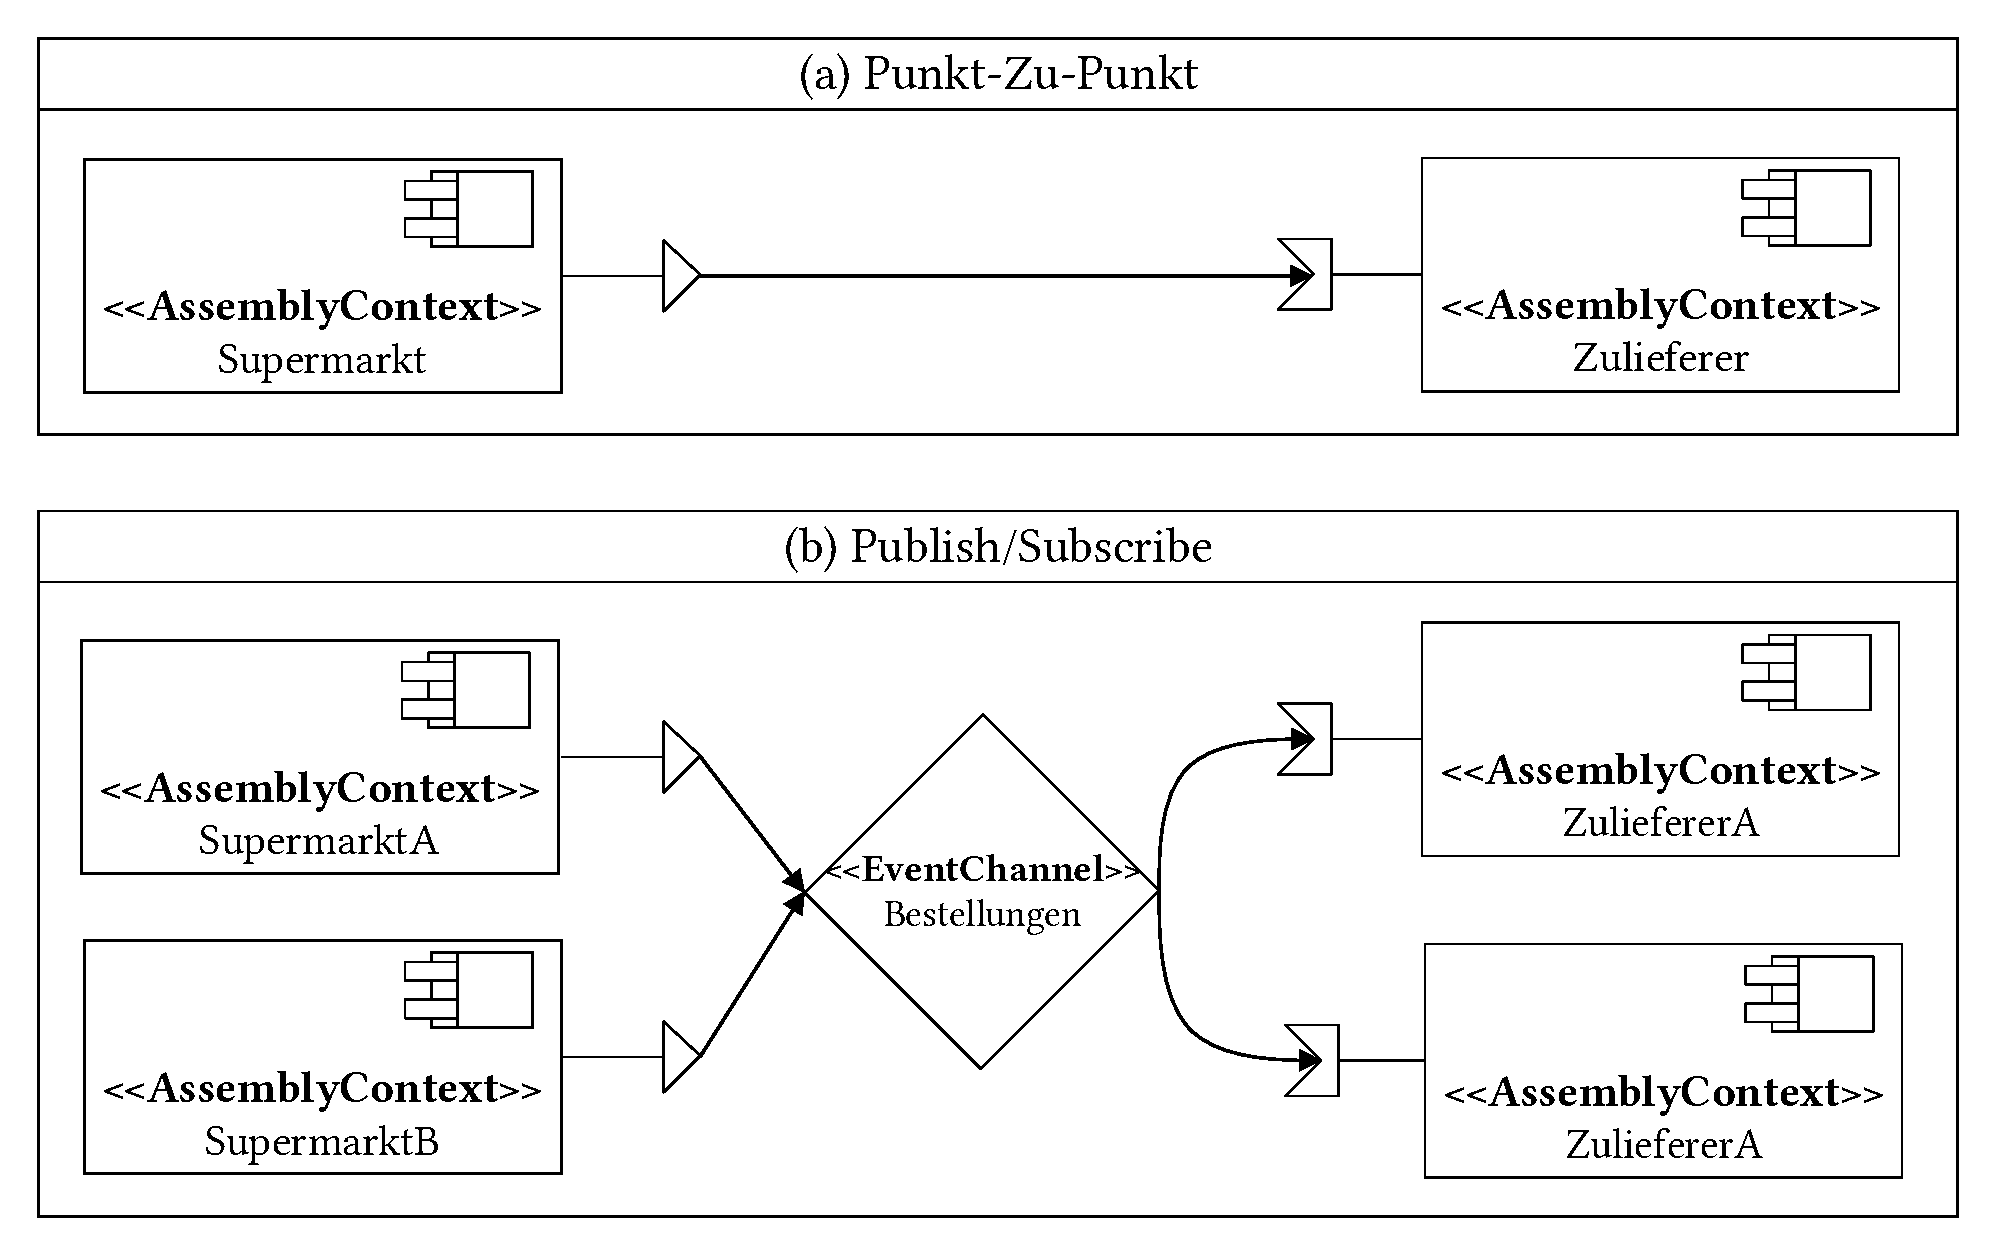
\includegraphics[width=1\textwidth]{images/grundlagen/grundlagenEventSystem.pdf}
  \caption{Punkt-Zu-Punkt und Publish/Subscribe im PCM.}
  \label{img:grundlageneventssystem}
\end{figure}



\subsection{Integrierung event-basierter Kommunikation in PCM}
\label{sec:eventbasetransformation}
Ein Software-Architekt muss für eine bestimmte Architektur die Auswirkungen verschiedener Middleware-Produkte oder Konfigurationen desselben Produkts abschätzen können. Die Palladio-Bench führt im Rahmen der Simulation eine Modelltransformation durch, um ein Middleware-Repository in das Architekturmodell einzubinden. Dieses Middle\-ware-Repository ist ein wiederverwendbares Modell und kann, wenn es einmal modelliert wurde, in verschiedene Architekturen eingewebt werden. Dieses Middleware-Repository kann vom Software-Architekten in zwei Arten beeinflusst werden. Zum einen kann er in der Ausführungsumgebung eine Middleware-Ressource angeben, auf der die Middleware bereitgestellt wird. Zum anderen kann er Middleware-Komponen\-ten spezifizieren, die Middleware spezifische Schnittstellen implementieren. Anhand dieser Schnittstellen, werden die Komponenten schließlich in die Gesamtarchitektur eingewoben. Dies geschieht in der Modelltransformation. Bei dieser wird die ursprüngliche event-basierte Kommunikation durch eine generische Komponentenkette ersetzt. Diese stellt den Datenfluss zwischen der Sender und der Empfänger Komponente dar. Diese Komponentenkette beinhaltet keine Ressourcenanforderungen. Diese sind in der konkreten Middleware-Modellierung, im Middleware-Repository, enthalten. Die Komponentenkette definiert außerdem die bereits erwähnten Schnittstellen die das Middleware-Modell implementieren kann. Wenn bei der Transformation eine Komponente aus dem Middleware-Modell eine dieser Schnittstellen bereitstellt, wird sie in die generische Komponentenkette eingebunden. Ansonsten wird nichts eingewebt.

Die \autoref{img:weaving} zeigt die verfügbaren Schnittstellen und die Position in der Komponentenkette. Dabei sind die Namen und Parameter der Schnittstellen fest vorgegeben. 

\begin{figure}
\center
  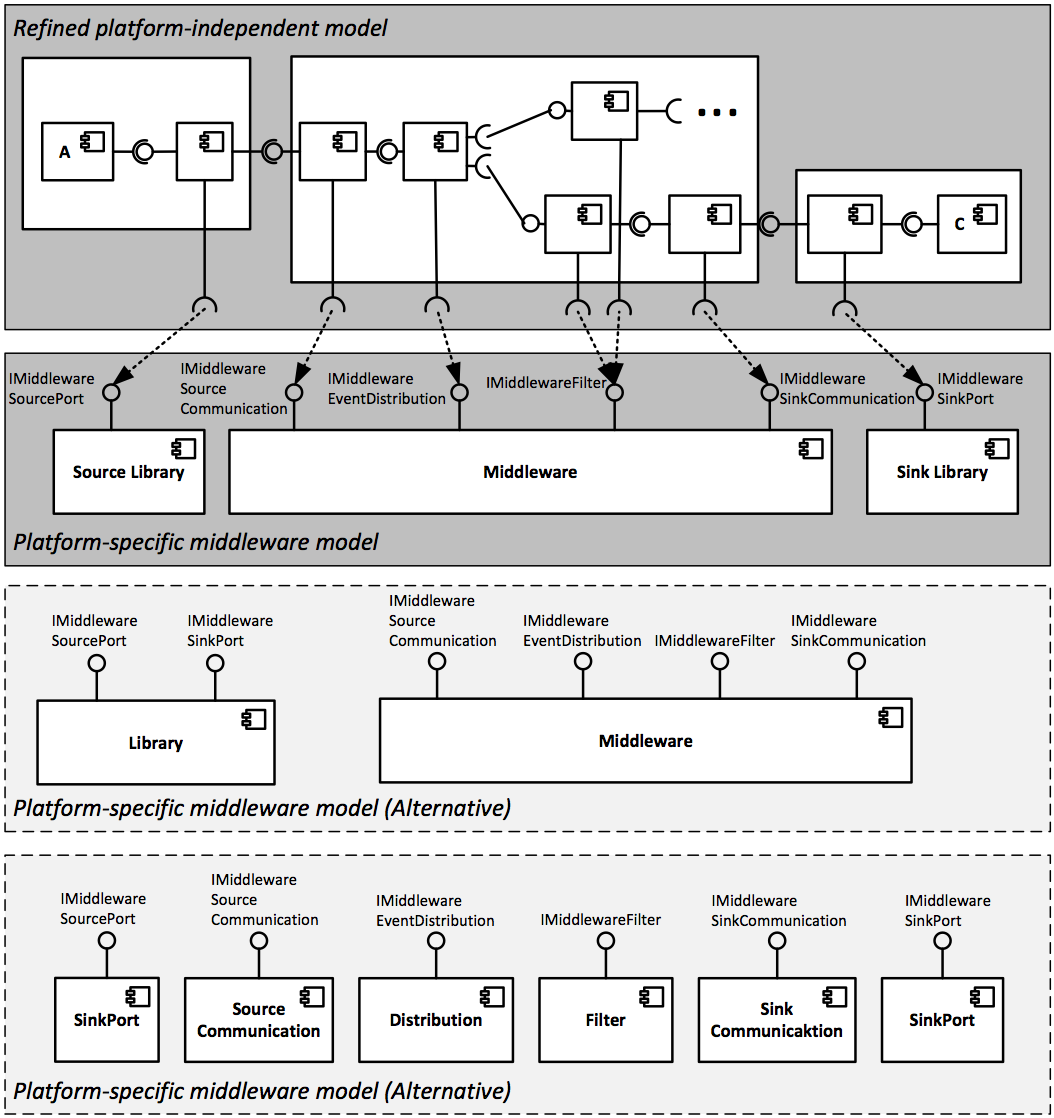
\includegraphics[width=1\textwidth]{images/grundlagen/middleware-model-weaving.png}
  \caption{Middleware-Schnittstellen, Komponenten und mögliche Alternativen, aus \cite{Rathfelder2013}}
  \label{img:weaving}
\end{figure}


\subsection{Performance-Analyse}
Die Palladio-Bench bietet eine Sammlung von Qualitätsanalysen mit Hauptfokus auf Performance an. Daneben gibt es auch Zuverlässigkeits- und Kostenanalysen. Jedes Analysewerkzeug hat seine Vor- und Nachteile. Außerdem unterscheiden sie sich in ihrer Genauigkeit, Geschwindigkeit und ihrem Funktionsumfang. Im Palladio Kontext ist ein Analysewerkzeug eine Software, die eine Analysetechnik implementiert, die ein bestimmtes Analysemodell löst. Mit Lösen ist das Sammeln von Qualitätsmetriken aus dem Analysemodell gemeint. Diese Analysewerkzeuge können wie eine Blackbox verwendet werden, da ein Software-Architekt kein Spezialwissen, sondern nur Wissen über die Modellabstraktion, benötigt um ein Analysewerkzeug zu verwenden. Nachdem ein Software-Architekt ein Modell erstellt hat, kann er ein Analysewerkzeug auswählen, das ihm Qualitätsmetriken vorhersagt. Im Rahmen der Masterarbeit werden nur Performance-Analysen betrachtet.  Mithilfe des Analysewerkzeugs \emph{SimuCom} \cite{simucom} wurde im Rahmen der Masterarbeit die Performance von MOMs vorhergesagt. SimuCom berechnet verschiedene Performance Charakteristiken, darunter Antwortzeiten für Systeme und Komponenten. Außerdem wird die Auslastung der einzelnen Ressourcen berechnet. Für die Analyse transformiert SimuCom das Eingabemodell, mithilfe einer Modell-Zu-Text Transformation, in Java-Code. Der generierte Code wird im Anschluß an die Ausführungsumgebung von SimuCom angeschlossen und im nächsten Schritt ausgeführt. Nachdem die Simulation fertig ist, werden die Ergebnisse in der Palladio-Bench angezeigt. Dieser ganze Prozess ist vollautomatisch und benötigt keine Benutzerinteraktion. SimuCom wird im Rahmen der Masterarbeit bei der Modellierung und Evaluierung einer MOM verwendet.

\section{Benchmark}
Im Kontext der Informatik bezeichnet der Begriff Benchmark einen oder mehrere Tests, die ausgeführt werden, um die Leistungsfähigkeit von Computersystemen zu vergleichen. Hierfür wird zwischen verschiedenen Arten von Benchmarks unterschieden \cite{Lilja2004}. 
\begin{itemize}
\item \textbf{Mikrobenchmarks} sind Tests einzelner Komponenten ohne Interaktion mit dem Gesamtsystem. Mit ihnen kann beispielsweise festgestellt werden, ob die Leistungsfähigkeit aller Komponenten innerhalb eines Systems im Gleichgewicht ist. Das Erstellen von Mikrobenchmarks erfordert ein tiefes Verständnis der zu testenden Systemkomponente.

\item \textbf{Synthetische Benchmarks} sind Tests künstlicher Instruktionsfolgen. Die getesteten Instruktionsfolgen können dabei in realen Anwendung vorkommen, müssen aber nicht.

\item \textbf{Anwendungsbenchmarks} beschreiben vollständige Programme, welche repräsentativ für eine bestimmte Klasse von Anwendungen sind. Dieser Art von Benchmark kann am Besten das Verhalten eines Benutzers oder externen Systems widerspiegeln. Da Anwendungsbenchmarks sehr aufwändig sind, wird mithilfe von kleinen Eingabedaten versucht die Laufzeit zu reduzieren.
\end{itemize}
Im Rahmen der Masterarbeit wird ein Anwendungsbenchmark verwendet um eine MOM zu untersuchen.

%- warum sind benchmark sinnvoll? bestehendes und einheitliches system mit dem man sich und andere vergleichen kann!!




%% LaTeX2e class for student theses
%% sections/evaluation.tex
%% 
%% Karlsruhe Institute of Technology
%% Institute for Program Structures and Data Organization
%% Chair for Software Design and Quality (SDQ)
%%
%% Dr.-Ing. Erik Burger
%% burger@kit.edu
%%
%% Version 1.3.3, 2018-04-17

\chapter{Verwandte Arbeiten}
\label{ch:Verwandte}
Im Folgenden wird der aktuelle Forschungsstand bzgl. der Modellierung und Benchmarking von MOMs beschrieben. Dabei werden Arbeiten vorgestellt, die als Grundlage dieser Masterarbeit dienen, bzw. von denen sich diese Arbeit abgrenzt.

\section{Benchmarking und Leistungmodellierung}
Eine Übersicht über Techniken zum Benchmarking und zur Leistungsmodellierung von event-basierten Systemen wurde in \cite{Kounev2009} veröffentlicht. Als Benchmark wird dort der SPECjms2007 verwendet. Die verwendeten MOMs implementieren alle die JMS-Schnittstelle. \par
Happe et al. \cite{happe} stellen ein Verfahren zur Modellierung von nachrichtenbasierten Middleware-Systemen vor. 
%Mithilfe einer Modelltransformationen werden Low-Level-Details in High-Level-Software-Architekturmodelle integriert. 
Eine Fallstudie, die auf Teilen des SPECjms2007-Benchmarks basiert, wird als Validierung des Ansatzes verwendet. Dieser Ansatz erlaubt es jedoch nur, Punkt-zu-Punkt-Verbindungen zu modellieren. \par
In der Arbeit von Liu et al. \cite{Liu2005} werden Vorhersagen der Performance für komponentenbasierte Systeme getroffen. Die Systeme werden dabei in einem Java EE-Applikationsserver eingesetzt. Allerdings umfassen die Workloads nicht mehrere Nachrichtenaustausche oder verschiedene Arten von Interaktionen. \par
%Außerdem Nur für java enterprise und benchmarking manuell durchführen. Auf Implementierungsebene.\cite{Liu2005} \\ 
Die Arbeit von Sachs et al. \cite{Sachs2013} stellt Modellierungsmuster für die Performance von Warteschlangen oder Nachrichtenkanälen vor. Die Muster bilden dabei die verschiedenen Charakteristiken auf Petrinetze ab. Der Ansatz wird mithilfe des \\ SPECjms2007-Benchmark präsentiert und validiert. Mithilfe der Arbeit verringert sich die Lücke zwischen Architekturspezifikationen und Vorhersagemodell. Dennoch ist Expertenwissen erforderlich, da das Performance-Modell manuell erstellt werden muss. \par
In \cite{baldoni} wird ein Berechnungsmodell für Publish/Subscribe-Kommunikation vorgestellt. Dabei werden Übertragungen als Verzögerung angenommen. Basierend auf diesem Berechnungsmodell wird ein probabilistisches Modell für die Effektivität der Publish/Subscribe-Kommunikation abgeleitet. Performance-Metriken wie Übertra-\\gungszeit oder Ressourcenauslastung werden nicht berücksichtigt. \par
Der Ansatz aus \cite{Kounev2008} stellt auch eine Methodik zur Charakterisierung und Per\-formance-Modellierung von verteilten event-basierten Systemen vor. Dieser ist aber auf die Verfügbarkeit von Überwachungsdaten, aus dem laufenden System, angewiesen und daher nur anwendbar, wenn eine laufende Systemimplementierung vorhanden ist. \par
Alle in diesem Abschnitt vorgestellten Ansätze arbeiten auf sehr speziellen Analyse-Modellen. Die Anwendung der Ansätze erfordert deshalb detailiertes Expertenwissen. Dadurch wird die Integration in einen generellen Software-Entwicklungsprozess erschwert.  
%und  als der Ansatz der Masterarbeit, der bereits zu Modellierungszeit ohne großes Expertenwissen und ohne vorhandene Systemimplementierung den Softwarearchitekten unterstützen will.

\section{Performance-Messungen und Konfigurationsentscheidungen für MOMs}
\label{sec:config_mom}
In der Literatur finden sich verschiedene Arbeiten der jeweiligen MOM-Hersteller, die ihre MOM mit anderen MOMs vergleichen. In \cite{kafka} vergleichen die Autoren Apache Kafka mit den beiden MOMs ActiveMQ und RabbitMQ. Dabei wird die Performance der drei MOMs untersucht. Auch in der Arbeit von Dobbelaere et al. \cite{Dobbelaere2017} wird Kafka und RabbitMQ im Hinblick auf Performance und Verfügbarkeit verglichen. Dabei werden jeweils Benchmarks und die jeweiligen Standardkonfigurationen der MOMs verwendet. Außerdem präsentieren einige MOM-Hersteller, die Performance ihrer MOM auf ihrer Internetseite. In \cite{kafkaconfig} wird die Performance von Apache Kafka in mehreren Benchmarks ausgemessen und die Ergebnisse präsentiert. Auch in \cite{rabbitperf} werden die Ergebnisse des Benchmarks der MOM RabbitMQ präsentiert. Das Problem mit den Artikeln ist, dass diese schon mehrere Jahre alt sind, die MOMs aber weiterentwickelt wurden. Deshalb kann davon ausgegangen werden, dass die Performance-Messungen nicht mehr aktuell sind. Die Artikel bieten jedoch einen genauen Aufbau an, mit dem eine Messung nachgestellt werden kann. \par
MOMs haben eine Vielzahl an Konfigurationsmöglichkeiten. Es existiert sehr wenig Literatur darüber, welche Konfigurationsentscheidung zum Beispiel die beste Performance oder Verfügbarkeit bringt. Diese Informationen werden oft auf den jeweiligen Internetseiten, der MOM-Hersteller, in einem Beitrag geteilt. Einen solchen Beitrag bietet der Hersteller der MOM RabbitMQ an. In einer dreiteiligen Serie \cite{rabbitconfig} beschreiben die Autoren, neben allgemeinen Hinweisen zu Einstellungsmöglichkeiten, jeweils die optimale Konfigurationen für RabbitMQ, um hohe Performance oder Verfügbarkeit zu erhalten. Jedoch werden keine Performance-Messungen oder ähnliches angeboten.\par
%Auch die Hersteller von ActiveMQ bieten eine Beitrag über Performanztuning an \cite{activemqconfig}. Dort wird beschrieben wie durch Konfiguration der Durchsatz erhöht werden kann. Für Kafka bieten die Hersteller eine Artikel \cite{kafkaconfig} an, mit dem 2-Millionen Schreibzugriffe pro Sekunde möglich sind. 
Die hier erwähnten Arbeiten sollen dafür verwendet werden um eine Performance-Messung für RabbitMQ durchzuführen. Außerdem sollen damit Konfigurationen identifiziert werden, die ausschlaggebend für die Performance sind.

\section{Modellierung event-basierter Interaktion in komponentenbasierten Architekturen}
Wie bereits in den Grundlagen erwähnt, bietet die Dissertation von Rathfelder \cite{Rathfelder2013} einen Ansatz an, mit dem die Modellierung event-basierter Interaktionen auf Architekturebene ermöglicht wird. Dabei wird das Meta-Modell des PCM erweitert. Außerdem, wird mithilfe einer Modeltransformation eine Performance-Analyse ermöglicht. In der Arbeit wird der Ansatz anschließend mithilfe zweier Fallstudien validiert. Das Problem, der Arbeit ist, dass Warteschlangen nicht explizit betrachtet werden und bestimmte Effekte somit nicht abgebildet werden können. Im Gegensatz dazu sollen in dieser Masterarbeit die Warteschlangen einer Middleware explizit betrachtet werden, um diese Effekte abbilden zu können. Die in der Arbeit von Rathfelder eingeführten Elemente zum Modellieren event-basierter Kommunikation, sowie die verwendete Fallstudie, mit dem SPECjms2007-Benchmark, werden in dieser Masterarbeit wiederverwendet.
%% LaTeX2e class for student theses
%% sections/content.tex
%% 
%% Karlsruhe Institute of Technology
%% Institute for Program Structures and Data Organization
%% Chair for Software Design and Quality (SDQ)
%%
%% Dr.-Ing. Erik Burger
%% burger@kit.edu
%% burger@kit.edu
%%
%% Version 1.3.3, 2018-04-17


\chapter{Untersuchung von nachrichtenbasierter Middleware}
\label{ch:mom}
Um die Performance einer MOM, oder eines Software-Systems im Allgemeinen, vorhersagen zu können, benötigt man zunächst Informationen über die Struktur des Systems, sein Verhalten, seine Ausführungsumgebung und über die Benutzung. Dazu müssen die verschiedenen Palladio-Rollen relevante Einflüsse bestimmen können. Der Komponenten-Entwickler muss Ressourcen-Anforderungen und Fehlerraten bestimmen. Der Software-Verteilungs-Experte muss verfügbare Rechenleistung und Hardware bestimmen. Der Domänenexperte muss das Verhalten der Nutzer bestimmen. Schließlich muss der Softwarearchitekt fehlende Werte bestimmen und das Modell damit kalibrieren. Diese Modellkalibrierung ist ein wichtiger Bestandteil des Modellierungsprozesses. In \cite{palladio17} wird beschrieben, wie und mit welchen Techniken die verschiedenen Rollen diese Daten erhalten und die jeweiligen Modelle kalibrieren können. Modellkalibrierung ist dabei die Anreicherung von Modellen mit quantitativen Daten, wie Ressourcenbedarf. Die Daten können aus Messungen oder Vorhersagen stammen. Die Modellkalibrierung ist eine Vorbedingung der Performance-Analyse. Die Informationen die eine Rolle in den verschiedenen Phasen der Software-Entwicklung gewinnen kann sind unterschiedlich. Dieser Prozess lässt sich in drei Aktivitäten strukturieren: Design, Entwicklung und Betrieb. Während der Design-Aktivität existiert die Applikation nur auf dem Papier und die Daten, die gesammelt werden können sind Schätzungen. Je weiter die Software-Entwicklung fortgeschritten ist, desto mehr quantitative Daten werden verfügbar um die Modelle kalibrieren zu können. Schließlich kann im Betrieb, das Gesamtsystem und auch der Benutzer quantitative Daten liefern. 

Im Rahmen der Masterarbeit wurde eine MOM modelliert um in Performance-Analysen eingesetzt werden zu können. Dazu wurden, wie oben beschrieben, verschiedenen Daten gesammelt um das Modell kalibrieren zu können, damit eine Performance-Analyse ermöglicht wird. Dazu wurde zunächst eine bereits existierende MOM ausgewählt. Da sie sich somit im letzten Schritt der drei Software-Entwicklungsaktivitäten befindet, konnte das Gesamtsystem betrachtet und ausgemessen werden, um quantitative Daten zu sammeln. Für die Auswahl wurden zunächst in \autoref{sec:anforderungenMom} Anforderungen an die MOM definiert. Die ausgewählte MOM wird im Anschluss in \autoref{sec:rmq} vorgestellt. Die Ergebnisse der Ausmessung der MOM sind in \autoref{sec:rmqBenchmark} beschrieben. Mithilfe der Ergebnisse, werden die Modelle in \autoref{ch:modellierung} anschließend kalibriert.


\section{Anforderungen an MOMs}
\label{sec:anforderungenMom}
Da es eine Vielzahl von MOMs gibt, muss zunächst eine Auswahl stattfinden. Dazu werden im ersten Schritt der Masterarbeit Anforderungen erarbeitet, die ein MOM erfüllen muss, damit sie in Betracht kommt. Die folgenden Anforderungen sollen erfüllt werden:
\begin{itemize}
\item Die MOM soll \textbf{Open Source} sein.
\item Sie soll eine \textbf{weite Verbreitung} haben.
\item Die Verwendung soll \textbf{Programmiersprachen unabhängig} sein.
\item Es soll eine MOM betrachtet werden, die sich in \textbf{aktiver Entwicklung} befindet.
\item Verschiedene \textbf{Interaktionstypen} sollen unterstützt werden.
\item Sie soll einen \textbf{hohen Grad der Entkopplung}, bzgl. Raum, Zeit und Synchronisation haben.
\item Die MOM soll sowohl das Punkt-Zu-Punkt als auch Publish/Subscriber \textbf{Nachrichtenmodell} unterstüzen.
\end{itemize}
%- bestimmte Protokolle unterstuetzen \\ %(https://www.predic8.de/activemq-hornetq-rabbitmq-apollo-qpid-vergleich.htm)

%\section{Auswahl der MOMs}
%In diesem Schritt sollen zwei bis drei MOMs ausgewählt werden. Dabei sollen die zuvor erarbeiteten Anforderungen einbezogen werden. Da sich bereits im Rahmen des Proposals mit dem Thema auseinander gesetzt wurde, wurden bereits drei starke Kandidaten identifiziert, die die bereits erarbeiteten Anforderungen erfüllen.
Im Folgenden wird eine MOM untersucht, die diese Anforderungen erfüllt.

\section{RabbitMQ}
\label{sec:rmq}
RabbitMQ (RMQ) ist, mit 35\,000 aktiven Produktivumgebungen, eine der am weitesten verbreitete MOMs. 
RMQ ist Open-Source und wird seit 2007 immer weiter entwickelt \cite{rabbitmq}. Das Ziel von RMQ ist es, allgemein einsetzbar zu sein. Deshalb wird eine Vielzahl an Protokollen unterstützt, unter anderem das JMS-Protokoll. RMQ kann auf einem zentralen Knoten oder auf mehreren verteilten Knoten eingesetzt werden. Für den Nachrichtenaustausch verwendet RMQ Warteschlangen. Diese lassen sich unterschiedlich konfigurieren, zum Beispiel in ihrer Warteschlangenlänge. Das Kommunizieren zwischen Sender und Empfänger geschieht dabei nicht direkt über die Warteschlange. Nachrichten werden zunächst an einen sogenannten \emph{Exchange} (dt. Austausch) gesendet. Dieser ist für das richtige Weiterleiten an die passende Warteschlange verantwortlich. Dies geschieht mit Hilfe von Bindungen und Routing-Schlüsseln. In RMQ ist eine Bindung eine Verbindung zwischen einer Warteschlange und einem Exchange. RMQ unterscheidet zwischen vier verschiedenen Exchange-Typen:
\begin{itemize}
    \item \textbf{Direct}: Hierbei meldet sich eine Warteschlange mit einem bestimmten Routing-Schlüssel X beim Exchange an. Wenn eine Nachricht mit einem Routing-Schlüssel Y ankommt, wird sie nur an die Warteschlange gesendet, wenn die Routing-Schlüssel X und Y übereinstimmen.
    \item \textbf{Topic}: Die Warteschlange ist mithilfe einer Bindung mit einem Exchange verbunden. Nachrichten werden wieder anhand des Routing-Schlüssels weitergeleitet. Der Routing-Schlüssel muss nicht mehr genau passen, sondern muss ein bestimmtes Muster aufweisen.
    \item \textbf{Fanout}: Die ankommende Nachricht wird an alle mit dem Exchange verbundenen Warteschlangen gesendet. Der Routing-Schlüssel wird dabei ignoriert.
    \item \textbf{Header}: Dabei werden die Attribute des Nachrichtenkopfes verwendet, um die Nachricht weiterzuleiten.
\end{itemize}
Diese Architektur erlaubt verschiedene Interaktionstypen. Sowohl eins-zu-eins als auch viele-zu-viele Interaktionen sind möglich. Dabei können nicht nur mehrere Warteschlangen existieren, sondern auch mehrere Exchanges und jede der Komponenten kann auf einem anderen Knoten verteilt sein. Aufgrund dieser Architektur hat RMQ auch einen hohen Grad der Entkopplung. Sender und Empfänger müssen sich nicht kennen, sie kommunizieren lediglich über den Exchange miteinander. Weder der Sender noch der Empfänger müssen zur gleichen Zeit aktiv sein. Der Sender sendet Nachrichten an die Warteschlange und der Empfänger entnimmt sie, wenn er die dazu nötigen Ressourcen zur Verfügung hat. Schließlich müssen Sender und Empfänger nicht aufeinander warten, da sie über eine Warteschlange kommunizieren.
In \autoref{img:rmq_architecture} ist ein Beispiel für eine mögliche RMQ-Architektur und Kommunikation zwischen Sendern und Empfängern dargestellt. Dabei ist \emph{ExchangeA} vom Typ Direkt. Dieser ist mit der \emph{Bestellungs}-Warteschlange verbunden. \emph{ExchangeB} ist ein Topic-Exchange und mit \emph{Bestätiguns}-Warteschlange und der \emph{Statistik}-Warteschlange verbunden. Dabei unterscheiden sich die beiden Bindungen in ihrem Routing-Muster. EmpfängerA empfängt Nachrichten aus der \emph{Bestellungs}-Warteschlange und EmpfängerB Nachrichten aus der \emph{Bestätiguns}- und \emph{Statistik}-Warteschlange. Wenn ein Sender eine Nachricht an \emph{ExchangeA} sendet, wird diese in der \emph{Bestellungs}-Warteschlange abgelegt, wenn der Routing-Schlüssel der Nachricht mit dem Routing-Schlüssel der Warteschlange übereinstimmt. Wenn eine Nachricht an ExchangeB gesendet wird, wird anhand des Routing-Musters entschieden, ob die Nachricht an die \emph{Bestätiguns}- oder \emph{Statistik}-Warteschlange gesendet wird. 
\begin{figure}
\center
  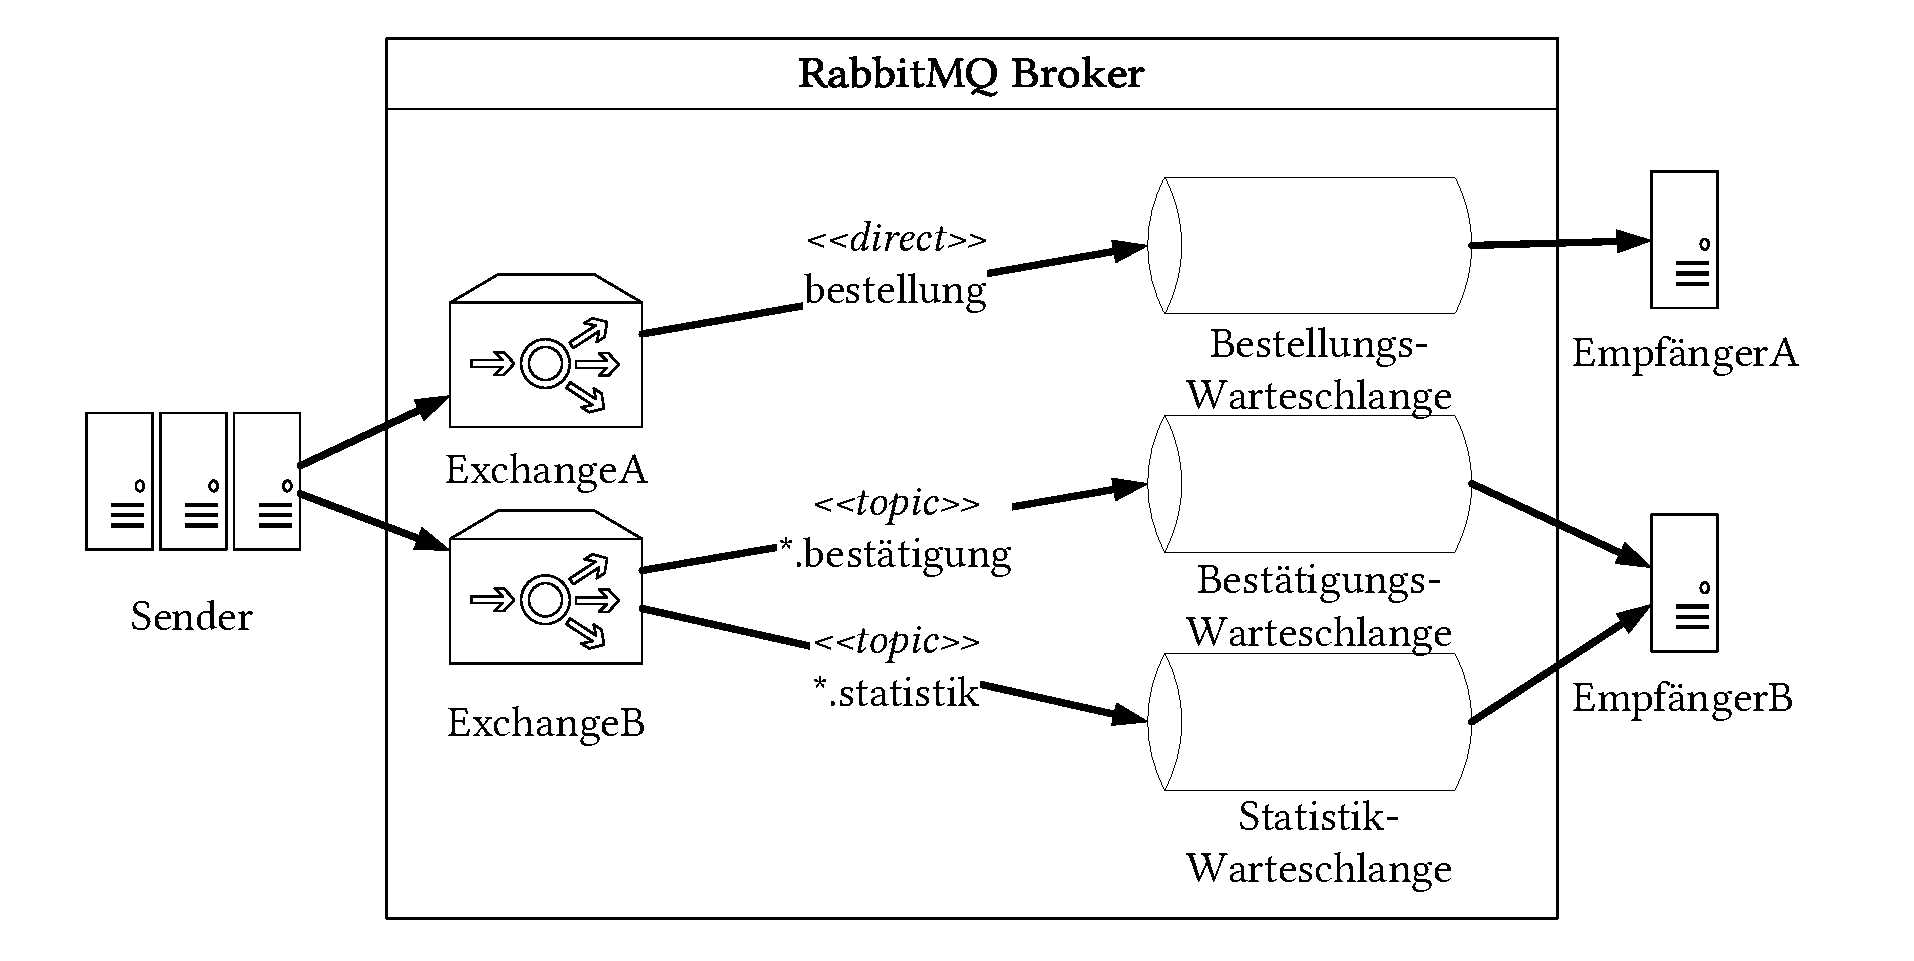
\includegraphics[width=1\textwidth]{images/measurement/rmqexample.pdf}
  \caption{Beispiel einer Kommunikation in RMQ}
  \label{img:rmq_architecture}
\end{figure}
%https://www.cloudamqp.com/blog/2015-05-18-part1-rabbitmq-for-beginners-what-is-rabbitmq.html

%https://www.cloudamqp.com/blog/2018-01-08-part2-rabbitmq-best-practice-for-high-performance.html
Da in dieser Arbeit der Fokus auf der Performance einer MOM liegt, wurde mithilfe von Literatur untersucht, für welche der beschriebenen Interaktionstypen, RMQ eine hohe Performance erreichen kann. Dazu konnten in (Rmqbuch) die folgenden Eigenschaften und Konfigurationsmöglichkeiten identifiziert werden. RMQ funktioniert am besten, wenn der Füllstand einer Warteschlange klein gehalten wird. Ein Nachricht die in eine leere Warteschlange abgelegt wird, geht direkt an einen Empfänger. Je mehr Nachrichten sich in der Warteschlange befinden, desto länger dauert es diese zu bearbeiten. Wenn der Durchsatz eine wichtige Rolle spielt und die Warteschlangen nicht voll laufen sollen, ist das Setzen einer maximalen Länge der Warteschlange oder das Setzen der Lebensdauer für Nachrichten empfohlen. Dabei bleibt die Warteschlange kurz und neue Nachrichten werden vom Kopf der Warteschlange verworfen, falls sie länger als festgelegt wird. Einen weiteren Performance-Einfluss haben Lazy-Warteschlangen. Dabei werden die Nachrichten einer Warteschlange direkt auf die Festplatte, anstatt in den Hauptspeicher, geschrieben. Das Ziel dabei ist, sehr lange Warteschlangen unterstützen zu können. Dies kann aus verschiedenen Gründen nötig sein:
\begin{itemize}
    \item Empfänger können aus verschiedenen Gründen ausfallen
    \item Plötzlicher anstieg ankommender Nachrichten
    \item Empfänger sind langsamer als normal
\end{itemize}
Das bedeutet, dass das Hauptziel von Lazy-Warteschlangen vor allem eine hohe Zuverlässigkeit ist. Da aber die Festplatte anstatt der Hauptspeicher verwendet wird, um die Nachrichten zu verwalten, ist diese Konfiguration langsamer. Im Fall, dass Performance bevorzugt wird, sollte also auf Lazy-Warteschlangen verzichtet werden. Der Unterschied von Lazy-Warteschlangen zu persistenten Nachrichten, die auch auf die Festplatte geschrieben werden, ist das bei persistenten Nachrichten der Sender entscheidet, ob die Nachricht persistiert wird. Bei Lazy-Warteschlangen, legt der Besitzer der Warteschlange fest, welche Nachrichten persisitiert werden. Der Durchsatz von RMQ kann außerdem dadurch erhöht werden, dass mehrere Warteschlangen verwendet werden. Zum Einen kann eine einzelne Warteschlange nicht mehr als ca. 50\,000 Nachrichten bearbeiten. Zum anderen sind Warteschlangen einfädig. Das heißt, dass der beste Durchsatz auf einem System möglich ist, wenn genau so viele Warteschlangen wie Kerne existieren. 

In der Folgenden Ausmessung von RMQ wurden diese und weitere Konfiguration untersucht um zu prüfen ob sie einen messbaren Einfluss auf die Performance haben.

\section{Benchmark}
Im Folgenden soll RMQ ausgemessen werden um quantitative Daten ableiten zu können. Dazu werden in \autoref{sec:testmachine} zunächst die Testmaschinen vorgestellt, mit denen die Messungen durchgeführt wurden. Im Anschluss werden in \autoref{sec:rmqBenchmark} die Ergebnisse der einzelnen Messungen vorgestellt und in \autoref{sec:rmqZusammenfassung} zusammengefasst.

\subsection{Testmaschinen}
\label{sec:testmachine}
Die Ausmessung wurde mit zwei virtuellen Servern durchgeführt, die von bwCloud \footnote{https://www.bw-cloud.org/} zur Verfügung gestellt wurden. Die Systemspezifikation der beiden Server ist in \autoref{tab:systespec} aufgelistet. Beide Systeme haben die gleiche Systemspezifikation und haben die RMQ Version 3.7.8 installiert. Für die Ausmessung wurden zwei Szenarien betrachtet. Der Aufbau dieser ist in \autoref{img:machineoverview} abgebildet. In \autoref{img:machineoverview}a ist der Fall zu sehen, bei dem sich Sender, Empfänger und RMQ auf der selben Maschine befinden. Damit soll RMQ unter den bestmöglichen Umständen ausgemessen werden. Dieses Szenario wird im Folgenden \textit{lokales}-Szenario bezeichnet. Das andere Szenario ist in \autoref{img:machineoverview}b zu sehen. Dabei befindet sich RMQ auf der einen Maschine und Sender und Empfänger auf der anderen. Damit sollen Netzwerkeffekte ausgemessen werden. Dieses Szenario wird im Folgenden \textit{entferntes}-Szenario bezeichnet. Die Netzwerklatenz zwischen beiden Systemen wurde durch eine zweiminütige Messung ermittelt. Die durchschnittliche Netzwerklatenz beträgt dabei 0,556 ms. 

\begin{table}
  \centering
  \begin{tabular}{|l|l|l|l|l|}
    Hauptspeicher & Festplatte & Anzahl vCPUs & GHz & Betriebssystem \\
    \hline
     4 GB & 15 GB & 2 & 2.4 GHz & Ubuntu 18.04
  \end{tabular}
	\caption{\label{tab:systespec} bwCloud VM Spezifikation}
\end{table}

\begin{figure}
\center
  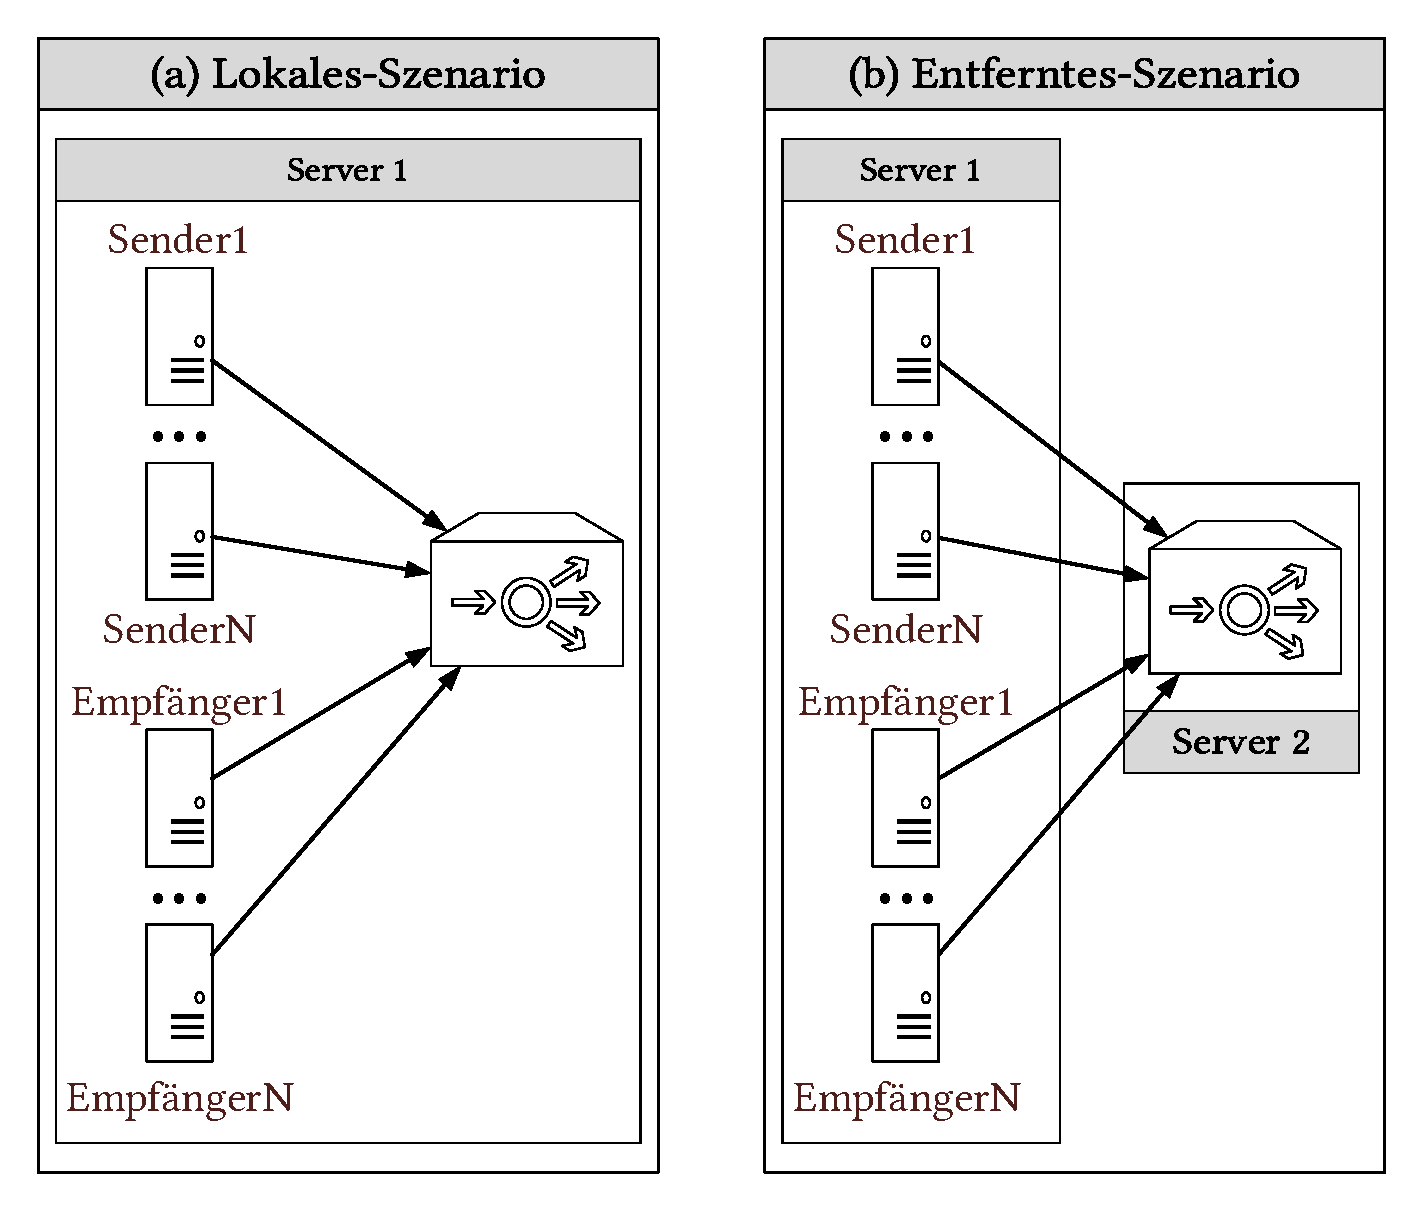
\includegraphics[width=1\textwidth]{images/measurement/benchmarkSzenarioOverview.pdf}
  \caption{Die Testszenarien: \textit{lokales}- und \textit{entferntes}-Szenario.}
  \label{img:machineoverview}
\end{figure}

\subsection{Ausmessung von RMQ}
\label{sec:rmqBenchmark}
Im Folgenden wird beschrieben, wie RMQ ausgemessen wurde, um mit den Ergebnissen die Modelle kalibrieren zu können. Um RMQ auszumessen wurde das Performance-Werkzeug von RMQ benutzt\footnote{https://github.com/rabbitmq/rabbitmq-perf-test}. Dieses erlaubt es, die gesendeten und empfangenen Nachrichten und ihre Latenz zu messen. Die Latenz ist hierbei als die Zeit definiert, die eine Nachricht braucht bis sie vom Empfänger aus der Warteschlange entnommen wird, nachdem sie vom Sender dort abgelegt wurde. Das Werkzeug kann konfiguriert werden um bestimmte Szenarien zu simulieren. Unter anderem lässt sich die Anzahl der zu sendenden und zu empfangenen Nachrichten pro Sekunde einstellen. Weitere Konfigurationsmöglichkeiten sind Nachrichtengröße und die Anzahl der Sender und Empfänger. Im Folgenden sollen die Ergebnisse der Messungen vorgestellt werden. Dabei werden die einzelnen Ergebnisse und ihr Versuchsaufbau vorgestellt. Jedes Ergebnis wird wie folgt beschrieben: 
\begin{itemize}
    \item Vorstellung des Szenarios
    \item Beobachtungen des Systemverhaltens
    \item Messergebnisse
\end{itemize}
Jede Messung wurde zehn mal durchgeführt. Die einzelnen Konfiguration wurde jeweils zwei Minuten ausgeführt. 



\subsubsection{Latenz einer nicht-persistenten Nachricht}
\label{sec:oneMsgLatency}
Zunächst soll geprüft werden wie groß die Latenz einer einzelnen, nicht persistenten, Nachricht ist. Dabei wurde auch die Größe einer Nachricht betrachtet. Dazu wurde die Senderate auf eine Nachricht pro Sekunde reduziert und die Nachrichtengröße zwischen 1 KByte und 1 MByte variiert. Für diese Messung wurde das \textit{lokale}-Szenario verwendet. Erwartet wird, dass die Latenz einer Nachricht mit ihrer Nachrichtengröße steigt.
%B
Die Ergebnisse sind in \autoref{img:senderate1-A} abgebildet. Neben den Messergebnissen ist eine Linie durch die Mediane der einzelnen Messungen gezogen. Dabei ist zu sehen, dass die Latenz einer Nachricht mit Ansteigen der Nachrichtengröße auch ansteigt. Somit verhält sich das System wie erwartet.
\begin{figure}
\center
  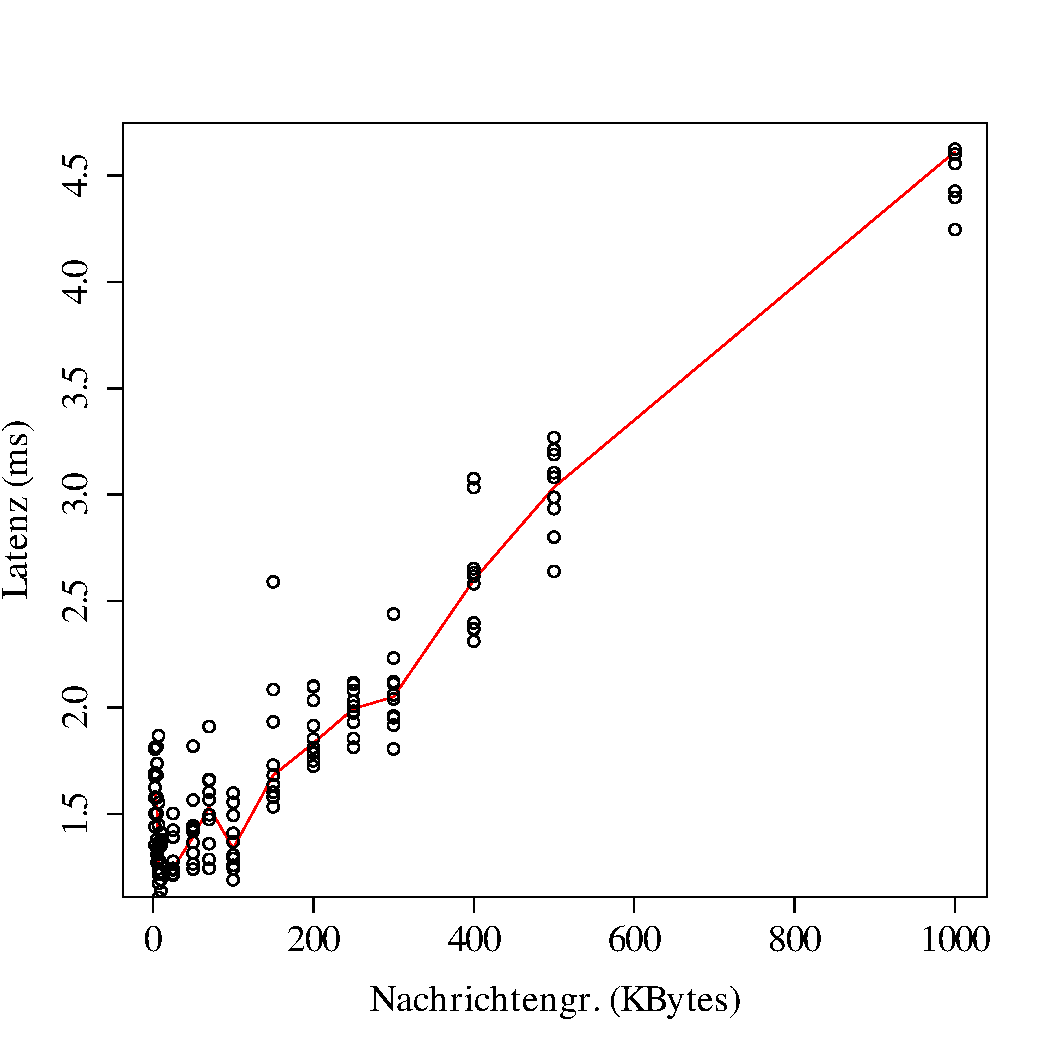
\includegraphics[width=0.7\textwidth]{images/measurement/rate-limit-1-A.pdf}
  \caption{Latenz einer nicht-persistenten Nachricht im \textit{lokal}-Szenario}
  \label{img:senderate1-A}
\end{figure}

Als nächstes wurde die Latenz einer Nachricht zu einer entfernten RMQ-Instanz gemessen. Dazu wurde das \textit{entfernte}-Szenario verwendet. Die Nachrichtengröße variiert zwischen 1 KByte und 1 MByte. Erwartet wird, dass zu der bereits gemessenen Latenz einer Nachricht die Netzwerklatenz dazugerechnet wird.

%B
Die Ergebnisse sind in \autoref{img:senderate1-B} zu sehen. Dabei ist durch die Mediane der einzelnen Messergebnisse eine Linie gezogen. Zu sehen ist, dass auch hier die Latenz mit Ansteigen der Nachrichtengröße wächst. Die Differenz, zur vorherigen Messung, entspricht der gemessenen Netzwerklatenz.
%E
Somit ist neben der Nachrichtengröße auch die Netzwerklatenz ein Faktor, der die Latenz einer Nachricht beeinflusst.

\begin{figure}
\center
  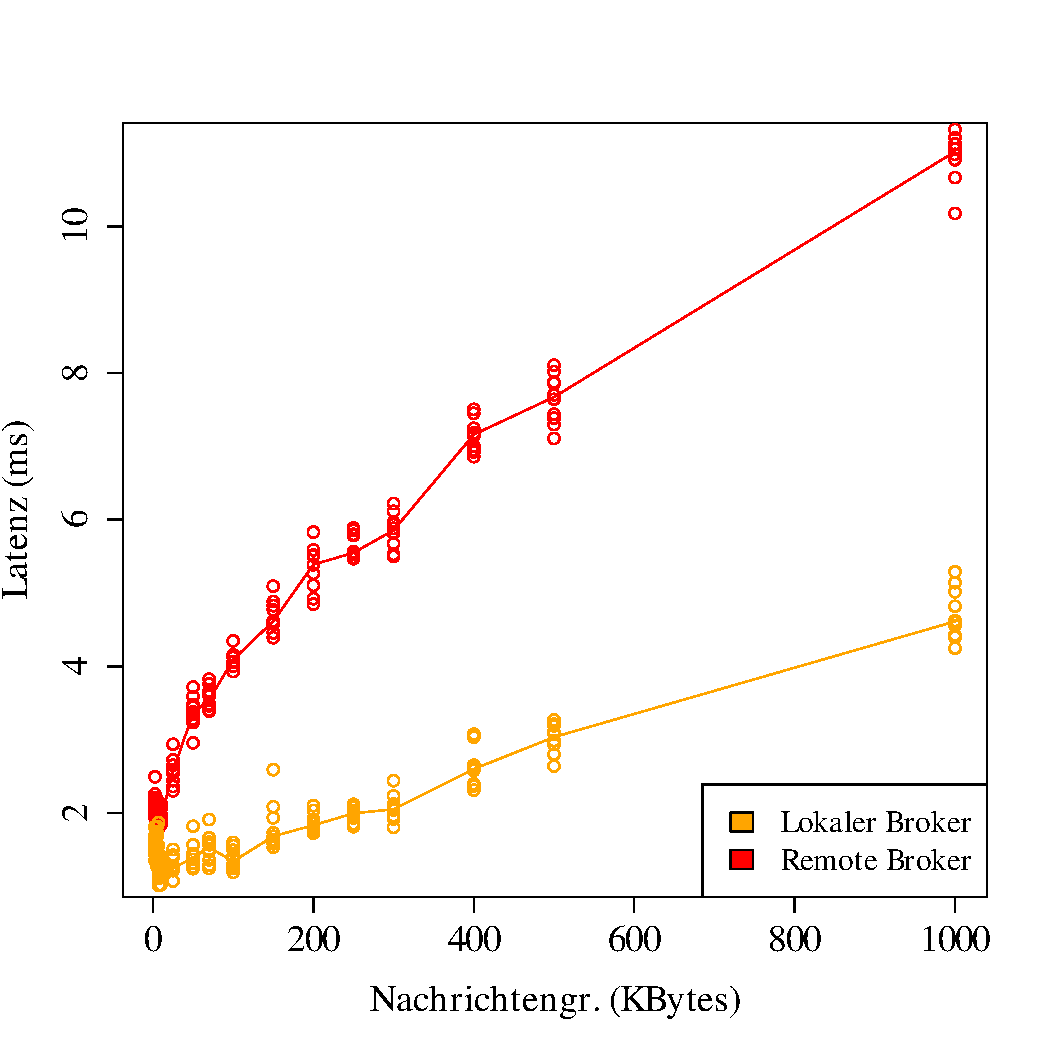
\includegraphics[width=0.7\textwidth]{images/measurement/rate-limit-1-AvsB.pdf}
  \caption{Vergleich der Latenz einer nicht-persistenten Nachricht im \textit{lokalen}- und \textit{entfernten}-Szenario}
  \label{img:senderate1-B}
\end{figure}

\subsubsection{Latenz einer persistente Nachricht}
Da zuvor die Latenz nicht-persistenter Nachrichten ausgemessen wurde, wird in dieser Messung die Latenz einer persistenten Nachricht ausgemessen. Die Senderate wurde auf eine Nachricht pro Sekunde reduziert und die Nachrichtengröße zwischen 1 KByte und 1 MByte variiert. Für diese Messung wurde das \textit{lokale}-Szenario verwendet. Erwartet wird, dass die Latenz einer persistenten Nachricht größer als die einer nicht-persistenten Nachricht ist, da die Nachricht auch auf die Festplatte geschrieben wird.
%B
In \autoref{img:senderatepersisten} sind die Ergebnisse der Messung zu sehen. Außerdem wurde zu Vergleich auch die nicht-persistente Messung eingezeichnet. Wie erwartet ist die Latenz einer persistenten Nachricht größer. Der Grund hierfür ist, dass die Nachricht auch auf die Festplatte geschrieben wird, um eine Zustellung zu garantieren. Somit hat die Wahl zwischen nicht-persistenten und persistenten Nachrichten einen Einfluss auf die Performance.

\begin{figure}
\center
  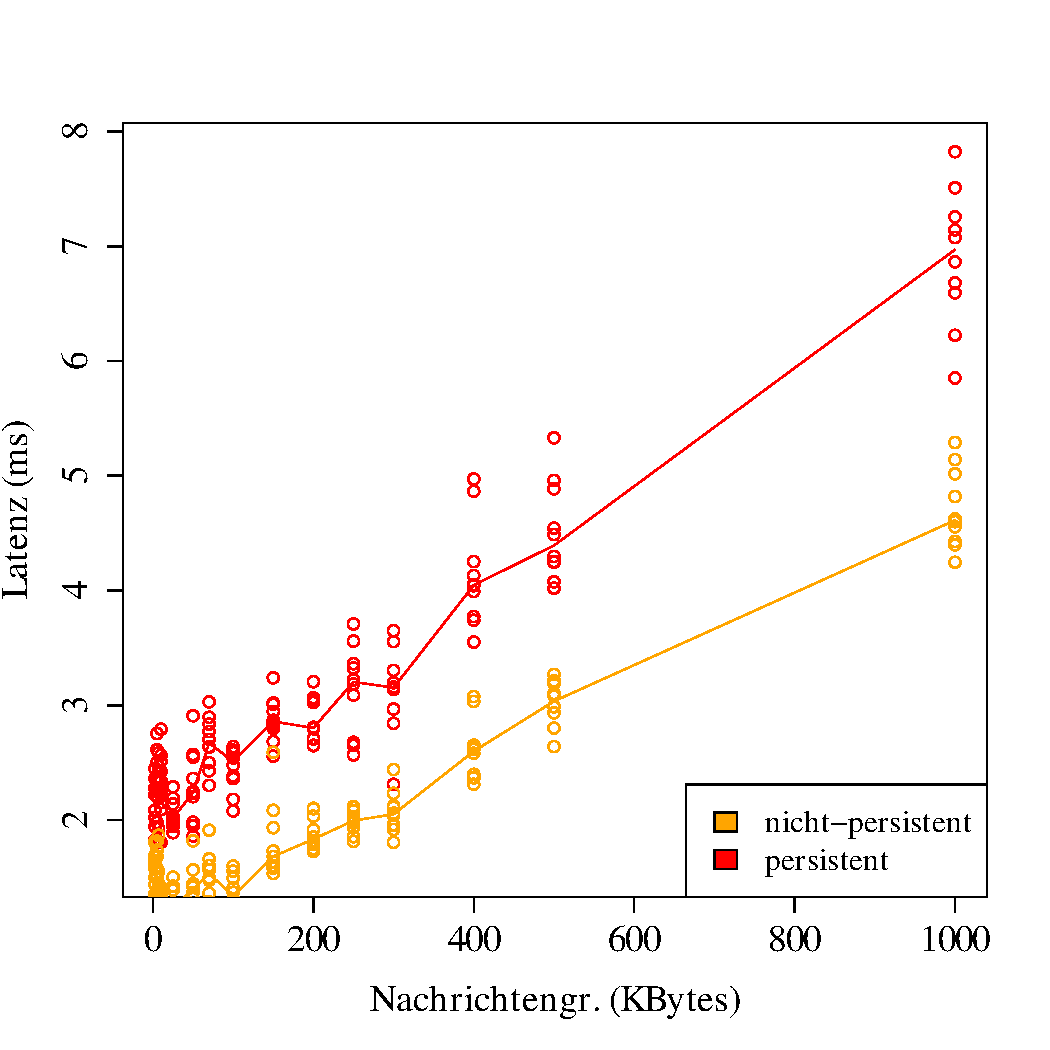
\includegraphics[width=0.7\textwidth]{images/measurement/persistentVsNonPersistent.pdf}
  \caption{Latenz einer nicht-persistenten im Vergleich zu einer persistenten Nachricht.}
  \label{img:senderatepersisten}
\end{figure}
\subsubsection{Nachrichtengröße}
Da in den vorherigen Messung die Nachrichtengröße als Einflussfaktor auf die Latenz und somit die Performance identifiziert wurde, sollen im Folgenden weitere Effekte im Zusammenhang mit der Nachrichtengröße untersucht werden. Dazu wurde ein Sender und ein Empfänger eingerichtet. Beide senden und empfangen Nachrichten so schnell sie können; die oben beschriebene Limitierung der Senderate auf eine Nachricht pro Sekunde ist somit aufgehoben. Die Nachrichtengröße variiert zwischen 1 KByte und 200 KByte. Es wurde mit dem \textit{lokalen}-Szenario ausgemessen. Erwartet wird, dass sich mit zunehmender Nachrichtengröße die insgesamt pro Sekunde gesendete Nachrichtenmenge verringert. Gleichzeitig sollte der Datendurchsatz zunehmen, da die Nachrichten weniger Routing-Overhead bei RMQ verursachen.
%B
In \autoref{img:msgsize} sind die Ergebnisse dieser Messung abgebildet. Durch die jeweiligen Mediane wurde eine Linie gezogen. Die Auswirkung der Nachrichtengröße auf die Senderate ist dabei in \autoref{img:msgsize}a zu sehen. Diese nimmt, wie erwartet, mit zunehmender Größe ab. In \autoref{img:msgsize}b ist der Datendurchsatz zu sehen. Auch hier verhält sich das System wie erwartet und der Datendurchsatz nimmt zu.
\begin{figure}
\center
  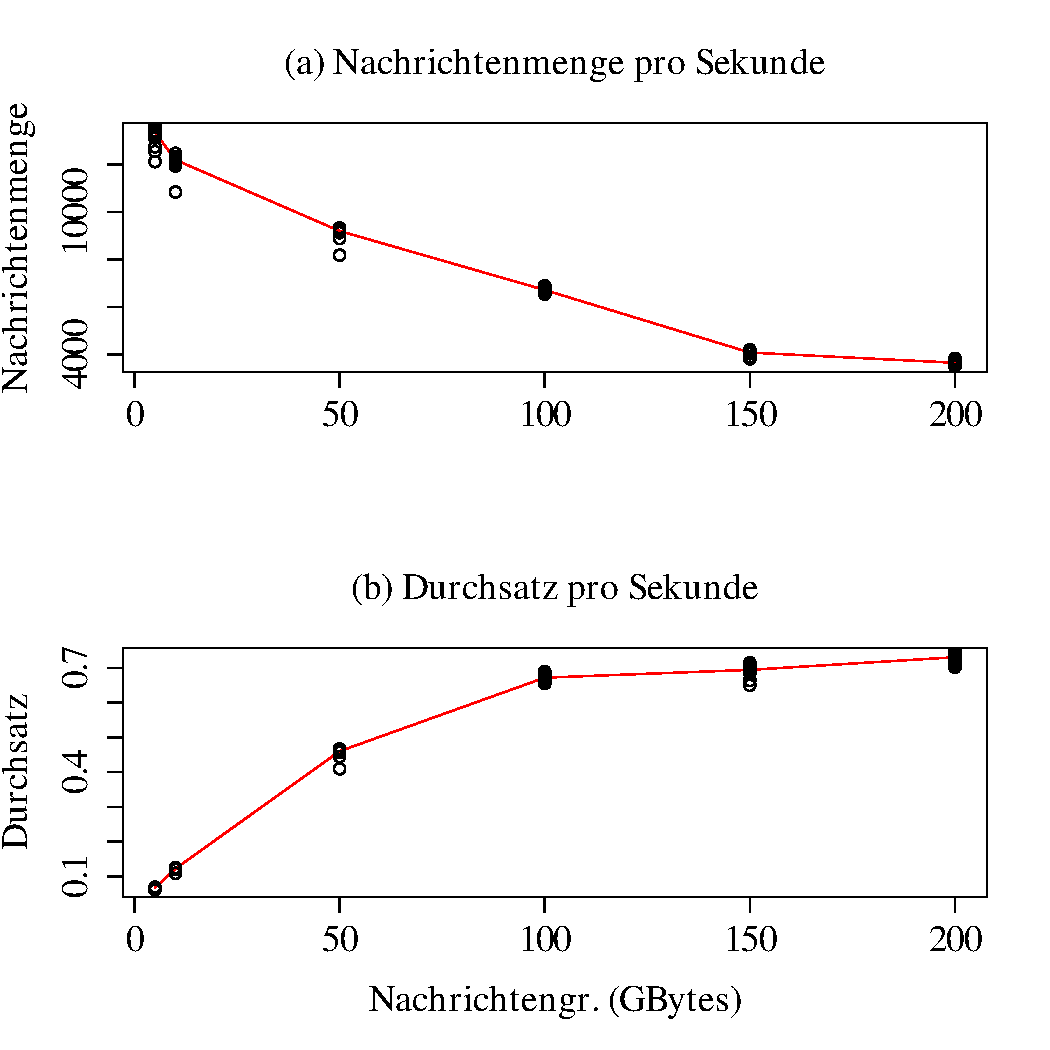
\includegraphics[width=0.7\textwidth]{images/measurement/msg-rate-vs-send-bytes.pdf}
  \caption{Nachrichtenmange und Durchsatz in Abhängigkeit der Nachrichtengröße.}
  \label{img:msgsize}
\end{figure}
%https://www.rabbitmq.com/blog/2012/04/25/rabbitmq-performance-measurements-part-2/

\subsubsection{Maximaler Datendurchsatz}
\label{sec:maxthroughput}
Nachdem die Effekte der zunehmende Nachrichtengröße geprüft wurden, soll nun geprüft werden wie groß der mögliche Datendurchsatz ist. Dazu wurden Nachrichten der Größe 1 KByte bis 200 KByte gesendet. Es wurden zwei Messungen durchgeführt. Im Fall der ersten Messung existiert ein Sender und kein Empfänger, bei der zweiten Messung ein Sender und ein Empfänger. Die Messung wurde mit dem \textit{lokalen}-Szenario durchgeführt. Erwartet wurde, dass die Messung ohne Empfänger einen höheren Durchsatz ermöglicht, da diese direkt verworfen werden. 
%B
Die Ergebnisse sind in \autoref{img:maxByteThroughputA} zu sehen. Die Abbildung zeigt, dass wenn kein Empfänger vorhanden ist, mit zunehmender Nachrichtengröße der Datendurchsatz sich einen Wert von ca. 1,5 GByte pro Sekunde annähert. Wenn ein Empfänger vorhanden ist, nähert sich der Datendurchsatz an 700 MByte pro Sekunde an. Dieser Unterschied lässt sich auf den fehlenden Empfänger bzw. die fehlende Warteschlange zurückführen. Es gibt somit keinen Schreib-Overhead, da die Nachricht weder im Speicher, noch auf der Festplatte abgelegt wird.
\begin{figure}
\center
  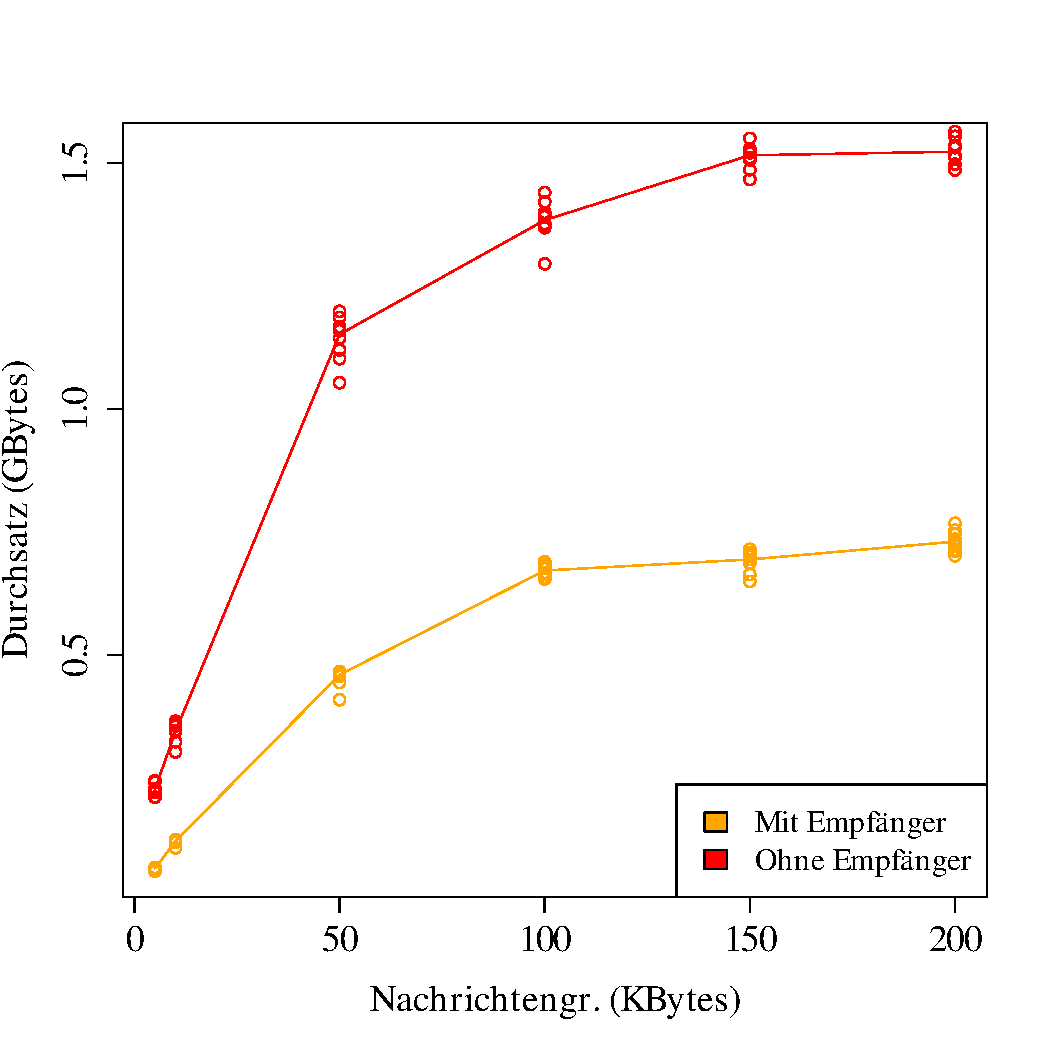
\includegraphics[width=0.7\textwidth]{images/measurement/rate-limit-unlimited-consumer-vs-no-consumer.pdf}
  \caption{Maximaler Durchsatz im \textit{lokalen}-Szenario.}
  \label{img:maxByteThroughputA}
\end{figure}

%Ein weiterer Effekt ist in \autoref{img:unlimitedLatency} zu sehen. Dabei ist zu sehen, dass die Latenz sinkt wenn mehr Nachrichten auf einmal gesendet werden.
%\begin{figure}
%\center
%  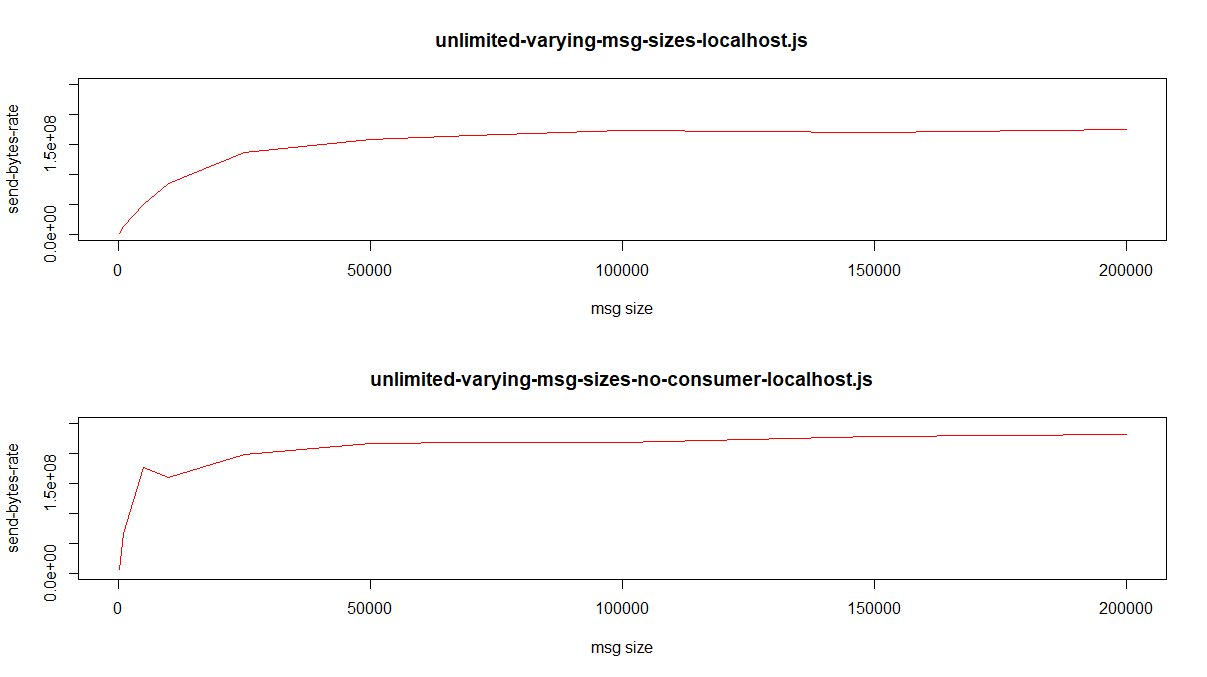
\includegraphics[width=1\textwidth]{images/max-byte-throughput-A.pdf}
%  \caption{Max Datenmenge, Latenz, Testsystem A}
%  \label{img:unlimitedLatency}
%\end{figure}
%Dieser Effekt laesst sich darauf zurueckfuehren, dass wenn mehrere Nachrichten auf einmal gesendet werden der Broker weniger routing overhead hat.

Die selbe Messung wurde mit dem \textit{entfernten}-Szenario durchgeführt. Erwartet wird, dass der Datendurchsatz kleiner ist, da die Netzwerkverbindung beachtet werden muss. 
%B
Die Gegenüberstellung für den Fall, dass es einen Sender, aber keine Empfänger gibt ist in \autoref{img:maxByteThroughputNoConsumerB} zu sehen. Der Datendurchsatz an das \textit{entfernte}-System ist dabei deutlich kleiner als zuvor. Diese nähert sich dem Wert von ca. 700 MByte anstatt 1,5 GByte an. Die Messung mit Empfänger ist in \autoref{img:maxByteThroughputB} abgebildet. Auch hier ist der Datendurchsatz deutlich kleiner und nähert sich nur einem Wert von ca. 400 MByte anstatt 700 MByte an.
\begin{figure}
\center
 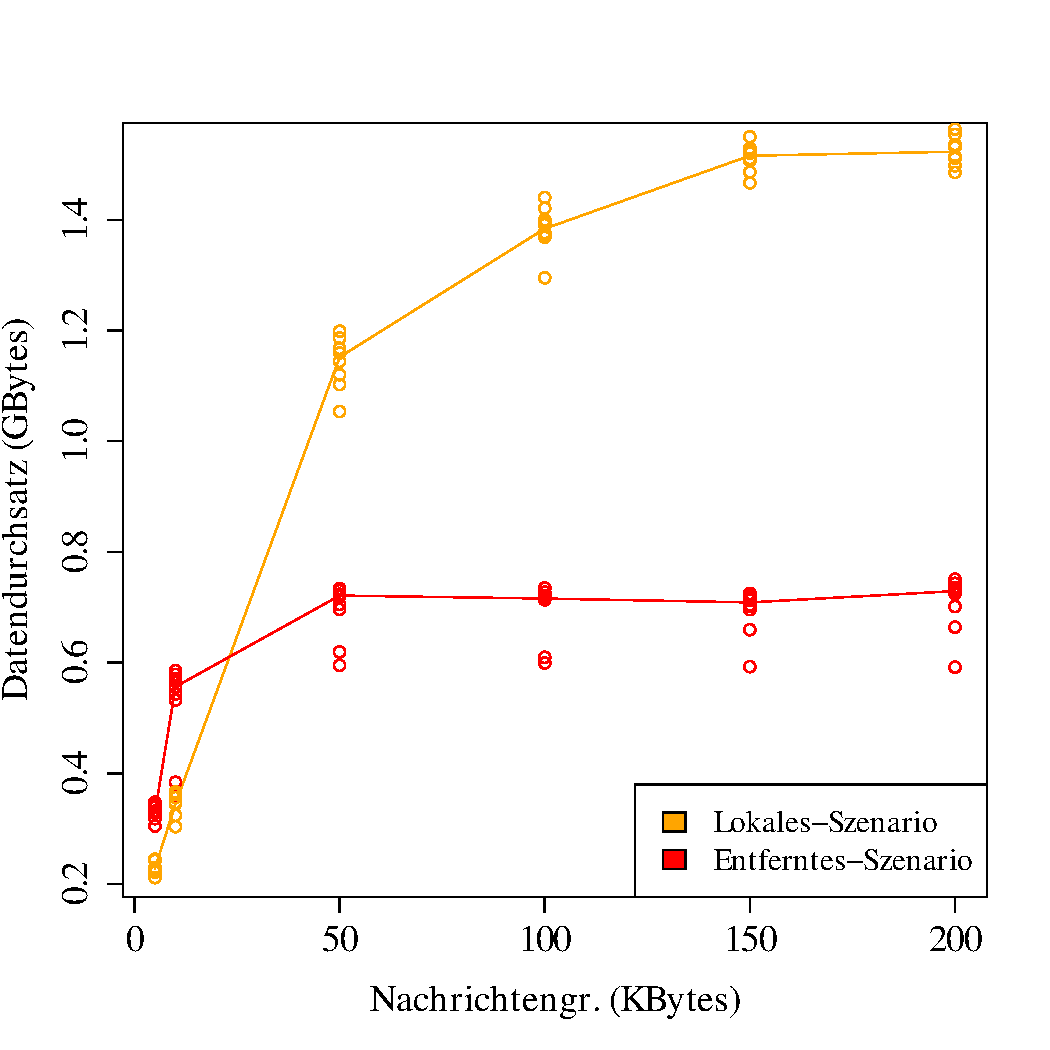
\includegraphics[width=0.7\textwidth]{images/measurement/rate-limit-unlimited-no-consumer-AvsB.pdf}
  \caption{Vergleich des maximalen Durchsatz ohne Empfänger zwischen dem \textit{lokalen}- und  \textit{entfernten}-Szenario.}
  \label{img:maxByteThroughputNoConsumerB}
\end{figure}
\begin{figure}
\center
 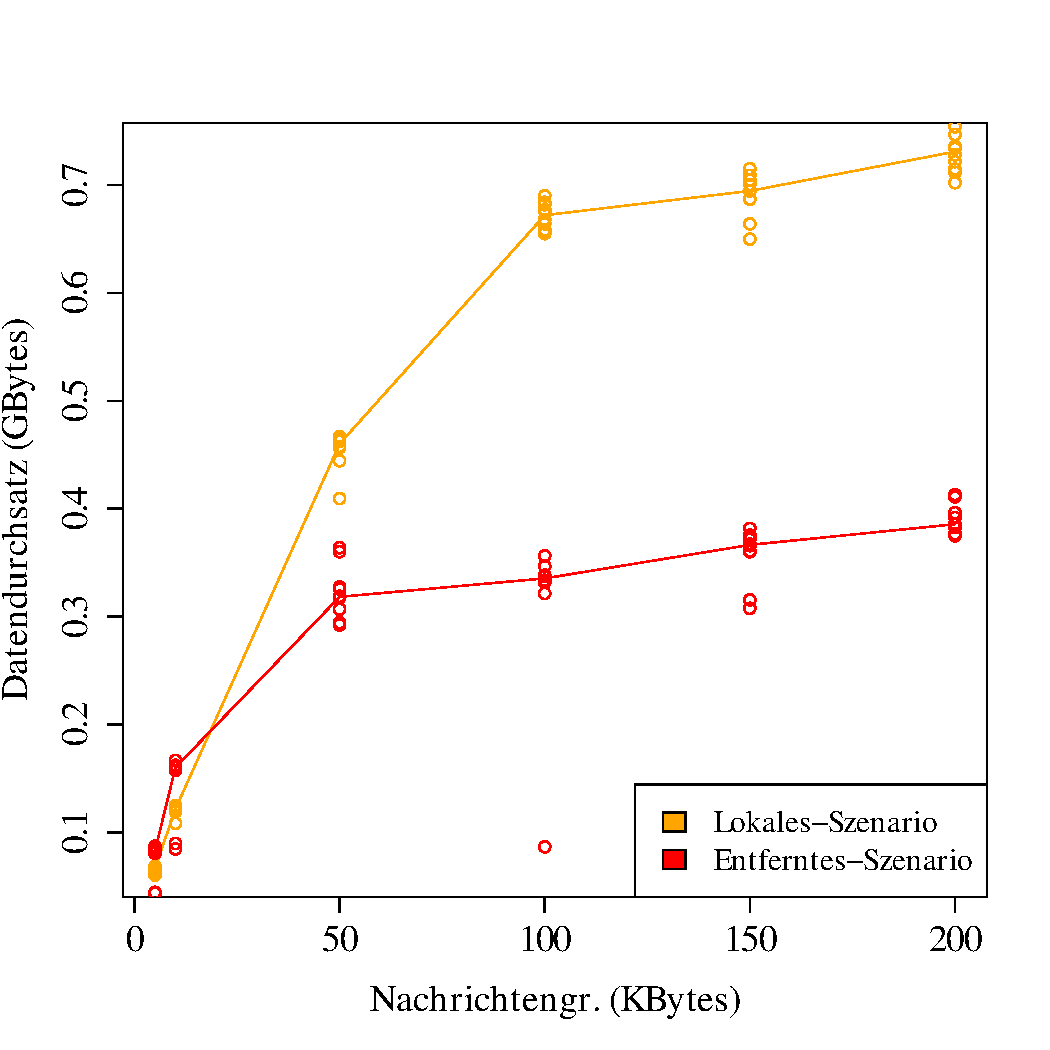
\includegraphics[width=0.7\textwidth]{images/measurement/rate-limit-unlimited-AvsB.pdf}
  \caption{Vergleich des maximalen Durchsatz mit Empfänger zwischen dem \textit{lokalen}- und  \textit{entfernten}-Szenario.}
  \label{img:maxByteThroughputB}
\end{figure}
%E
Obwohl beide Testmaschinen vom selben Anbieter sind, unterscheiden sich der mögliche Datendurchsatz zwischen einer lokalen und entfernten RMQ-Instanz. Dieser Unterschied kann auf den möglichen Durchsatz einer Netzwerkverbindung zurückgeführt werden. Somit ist der mögliche Durchsatz einer Verbindung zwischen Sender, Empfänger und RMQ ein limitierender Faktor und hat somit auch Einfluss auf die Performance des Gesamtsystems.

\subsubsection{Ansteigen des Füllstands der Warteschlange}
\label{sec:queueGrowth}
Diese Messung untersucht die Auswirkung des Warteschlangen-Füllstands auf die Latenz der einzelnen Nachrichten. Die Messung besteht aus einem Sender und einem Empfänger. Die Senderate beträgt zwei Nachrichten pro Sekunde, der Empfänger empfängt jedoch nur eine Nachricht pro Sekunde. Die Nachrichten sind dabei 1 KByte groß. Die Messung wurde mit dem \textit{lokalen}-Szenario durchgeführt. Erwartet wird, dass die Latenz der Nachrichten mit Ansteigen des Warteschlangenfüllstands wächst, da die Nachrichten länger in der Warteschlange warten, bis sie abgeholt werden.
%B
In \autoref{img:queuegrowth} sind die Messergebnisse abgebildet. Dabei ist in \autoref{img:queuegrowth}a der Füllstand der Warteschlange zu sehen. Diese wächst pro Sekunde um eine Nachricht die nicht abgeholt wird an. In \autoref{img:queuegrowth}b ist die Latenz der Nachrichten abgebildet. Wie erwartet steigt diese mit Ansteigen des Füllstands, da die Nachrichten länger in der Warteschlange warten müssen, bis sie abgeholt werden.
\begin{figure}
\center
  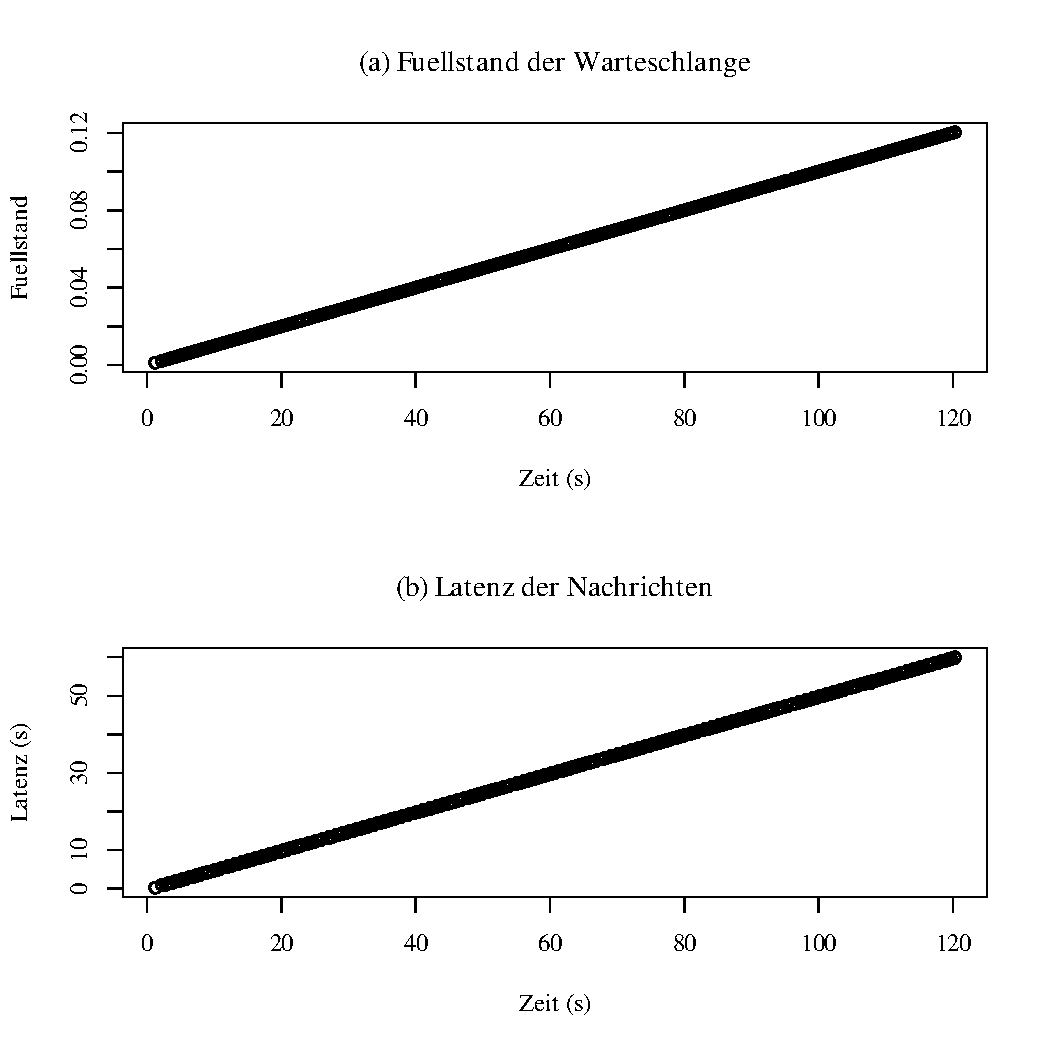
\includegraphics[width=0.7\textwidth]{images/measurement/queuegrowth.pdf}
  \caption{Wachstum einer Warteschlange und Auswirkung auf die Latenz.}
  \label{img:queuegrowth}
\end{figure}

\subsubsection{Konfiguration: Warteschlangenlänge begrenzen}
\label{sec:maxlength}
Die vorherige Messung hat gezeigt, das sich das Anwachsen der Warteschlange negativ auf die Latenz der Nachrichten auswirkt. Wie bereits erwähnt erlaubt RMQ einige Konfigurationen. Eine davon ist das Setzen einer maximal Länge für Warteschlangen. Damit soll die Warteschlange kurz gehalten werden und die Latenz der Nachrichten klein. Damit wird dem Effekt, der in der vorherigen Messung untersucht wurde, entgegengewirkt. Standardmäßig wird der Kopf der Warteschlange verworfen. Mit der folgenden Messung soll diese Konfiguration untersucht werden. Dazu wurden drei Warteschlangen angelegt. Diese hatten eine maximal Länge von 100, 5000 und 50.000 Nachrichten. Die Größe von 50.000 ist die RMQ-Standardgröße für Warteschlangen. Damit man die Auswirkung auf volle Warteschlangen sehen kann wurde die Sende- und Empfangsrate entsprechend angepasst. Die Senderate wurde auf 1000 und die Empfangsrate auf 100 Nachrichten pro Sekunde eingestellt. Die Nachrichten Größe war 100 Bytes. Die Messung wurde mit dem \textit{lokalen}-Szenario durchgeführt. Erwartet wird, dass sobald die Warteschlange voll wird, die Latenz nicht mehr zu nimmt. Dieser Moment sollte schneller erreicht werden, je kleiner die Warteschlange ist.
%B
Die Ergebnisse sind in \autoref{img:maxlength} abgebildet. Wie erwartet wachsen die Latenzen der Nachrichten bei den begrenzten Warteschlangen ab einem bestimmten Moment nicht weiter an. Wie in \autoref{img:maxlength}a und \autoref{img:maxlength}b zu sehen ist, tritt dieser Moment für die kürzere Warteschlange früher ein. In \autoref{img:maxlength}c wächst die Latenz immer weiter.
\begin{figure}
\center
  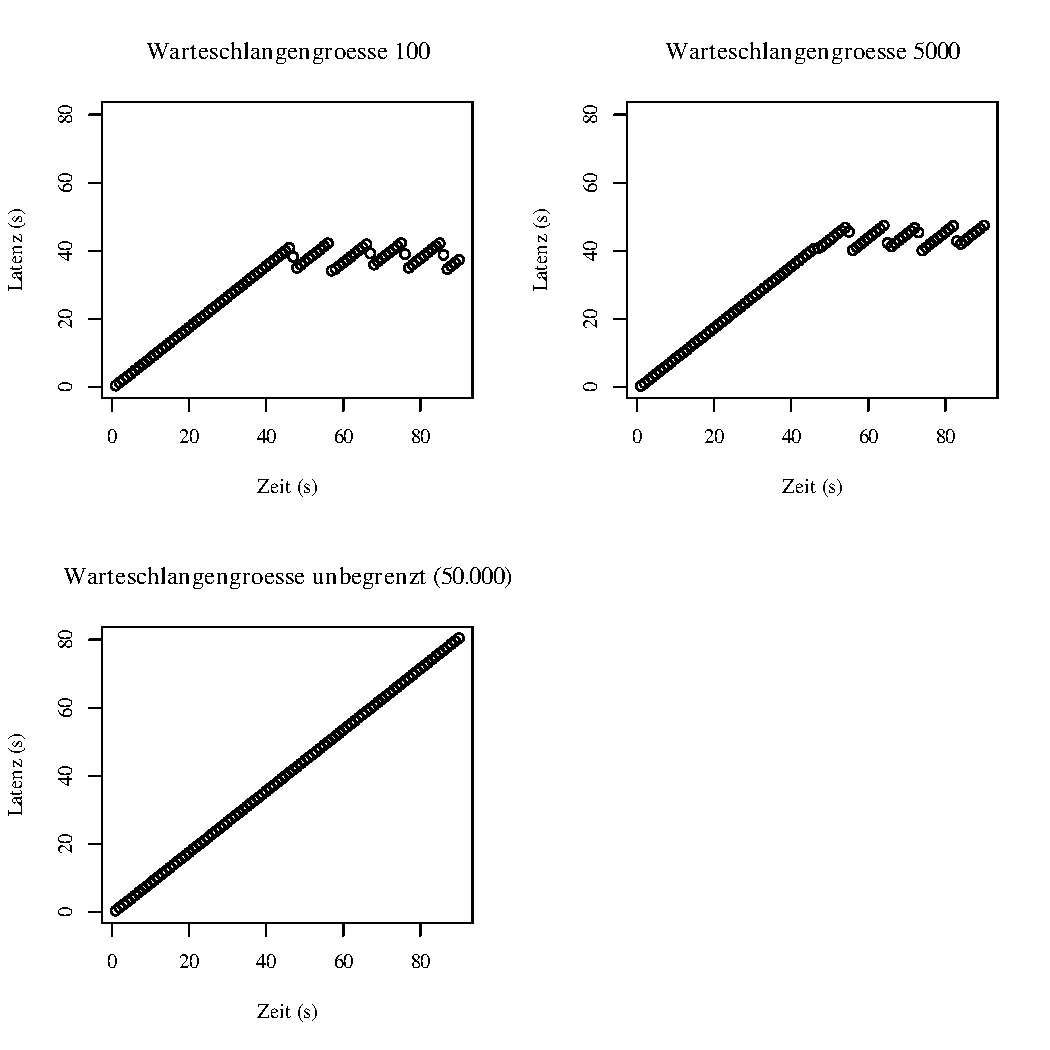
\includegraphics[width=0.7\textwidth]{images/measurement/max-length.pdf}
  \caption{Auswirkung auf die Latenz bei verschieden großen Warteschlangen.}
  \label{img:maxlength}
\end{figure}
%E
Diese Konfiguration zeigt, dass die Begrenzung der Warteschlangengröße einen Einfluss auf die Latenz hat, da man sie damit begrenzen kann. Der Nachteil dabei ist, dass Nachrichten verworfen werden, sobald die Warteschlange voll ist. Somit hat auch die Warteschlangengröße einen Einfluss auf die Performance. 

%wenn Queue voll, dann wird Msgrate angepasst

%Flow alarm ab RabbitMQ 2.8.0+ bei Versionen davor verhlaehlt sich RMQ wie in (sec: Speicher ausgeschoepft)

%\subsubsection{Speicher von RMQ ausgeschoepft}
%Nachdem in der Messung davor die Laenge der Warteschlange betrachtet wurde, soll nun untersucht werden ob der Verfuegbare Speicher des Broker einfluss auf die Performanz hat. Dazu wurde auf der Testmaschine B die Hauptspeicher fuer RMQ auf 10 MB gesetzt.  
%Sollte der verfuegbare Speicher des Broker ausgeschoepft sein, wird der MemoryAlarm aktiviert und der Broker blockiert ankommende Nachrichten, bis der Speicher wieder frei ist. Dies ist in (abb) zu sehen.
%TODO beobachtung und Ergebnis



\subsubsection{Konfiguration: Lazy-Warteschlangen}
\label{sec:rmqLazy}
Eine weitere Konfiguration die RMQ ermöglicht sind Lazy-Warteschlangen. Wie bereits erwähnt, werden dabei Nachrichten auf die Festplatte anstatt in den Hauptspeicher geschrieben. Dabei wird kein Unterschied gemacht ob die ankommenden Nachrichten persistent oder nicht-persistent sind. In der nächsten Messung soll untersucht werden ob die Konfiguration von Lazy-Warteschlangen Auswirkungen auf die Performance hat. Dabei wurde auch die Größe einer Nachricht betrachtet. Für die Messung wurde die Senderate auf eine Nachricht pro Sekunde reduziert und die Nachrichtengröße zwischen 1 KByte und 1 MByte variiert. Für diese Messung wurde das \textit{lokale}-Szenario verwendet. Erwartet wird, dass die Latenz einer Nachricht, im Vergleich zu nicht-persistenten Nachrichten größer ist. Außerdem sollte die Messung ähnliche Ergebnisse liefern wie die Messung mit persistenten Nachrichten.
%B
In \autoref{img:lazy} ist ein Vergleich der Messung mit nicht-persistenten und den Messergebnissen mit Lazy-Warteschlangen abgebildet. Zu sehen ist, dass die Latenz mit Lazy-Warteschlangen größer ist, als die der nicht-persistenten Nachrichten. Außerdem sind die Messergebnisse dieser Messung und der Messung mit persistenten Nachrichten ähnlich.
\begin{figure}
\center
  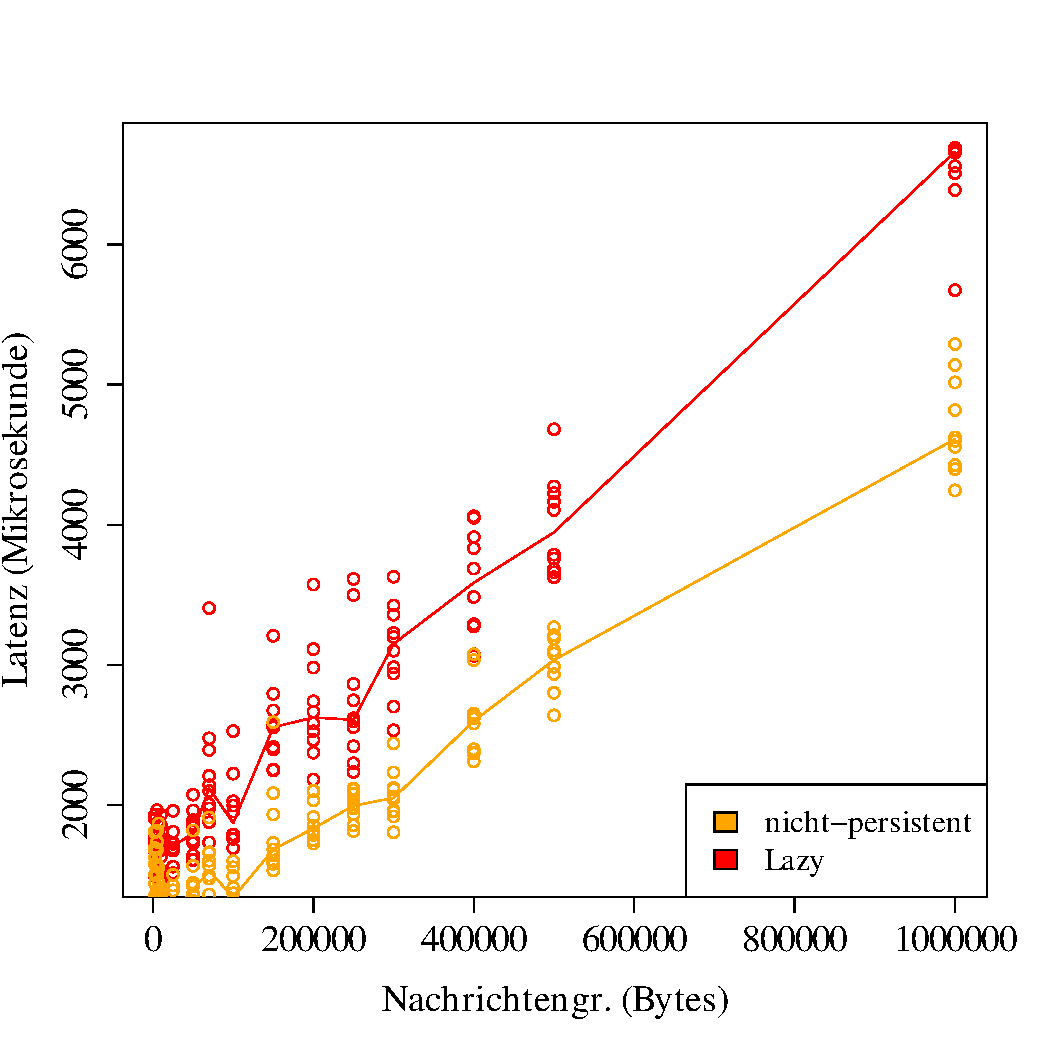
\includegraphics[width=0.7\textwidth]{images/measurement/lazy-queues.pdf}
  \caption{Lazy-Warteschlange im Vergleich mit nicht-persistenten Nachrichten.}
  \label{img:lazy}
\end{figure}
%E
Grund hierfür ist, dass die Nachrichten auf die Festplatte anstatt in den Hauptspeicher geschrieben werden. Somit hat diese Konfiguration einen ähnlichen Einfluss auf die Performance, wie der Einsatz persistenter Nachrichten.



\subsubsection{Mehrere Empfänger}
\label{sec:varyingConsumer}
In \autoref{sec:queueGrowth} und \autoref{sec:maxlength} war bereits zu sehen, dass volle Warteschlangen einen Einfluss auf die Latenz haben. In dieser Messung soll geprüft werden, ob es einen Unterschied macht, einen oder mehrere Empfänger eine Warteschlange abarbeiten zu lassen. Dazu wurde die Senderate eines Senders auf 1000 Nachrichten und die Empfangsrate auf 200 Nachrichten pro Sekunde limitiert. Alle Empfänger greifen auf die selbe Warteschlange zu. Außerdem wurde eine Referenzmessung mit einem Sender und einem Empfänger mit einer Sende- und Empfangsrate von 1000 durchgeführt. Die Messung wurde mit dem \textit{lokalen}-Szenario durchgeführt. Erwartet wird, dass es keinen Unterschied macht ob ein oder mehrere Empfänger eine Warteschlange abarbeiten.
%B
In \autoref{img:varyingConsumer} sind die Ergebnisse der Messung zu sehen. \autoref{img:varyingConsumer}a zeigt dabei einen Empfänger der alleine die Nachrichten empfängt. Da der Empfänger die Nachrichten nicht schnell genug empfängt, steigt die Latenz. In \autoref{img:varyingConsumer}b kommt ein weiterer Empfänger hinzu. Die Latenz wächst nicht ganz so schnell. \autoref{img:varyingConsumer}c zeigt fünf Empfänger die gemeinsam die Warteschlange abarbeiten. Im Vergleich zu der Referenzmessung in \autoref{img:varyingConsumer}d mit einem Empfänger, streut die Messung mit mehreren Empfängern stärker.
\begin{figure}
\center
  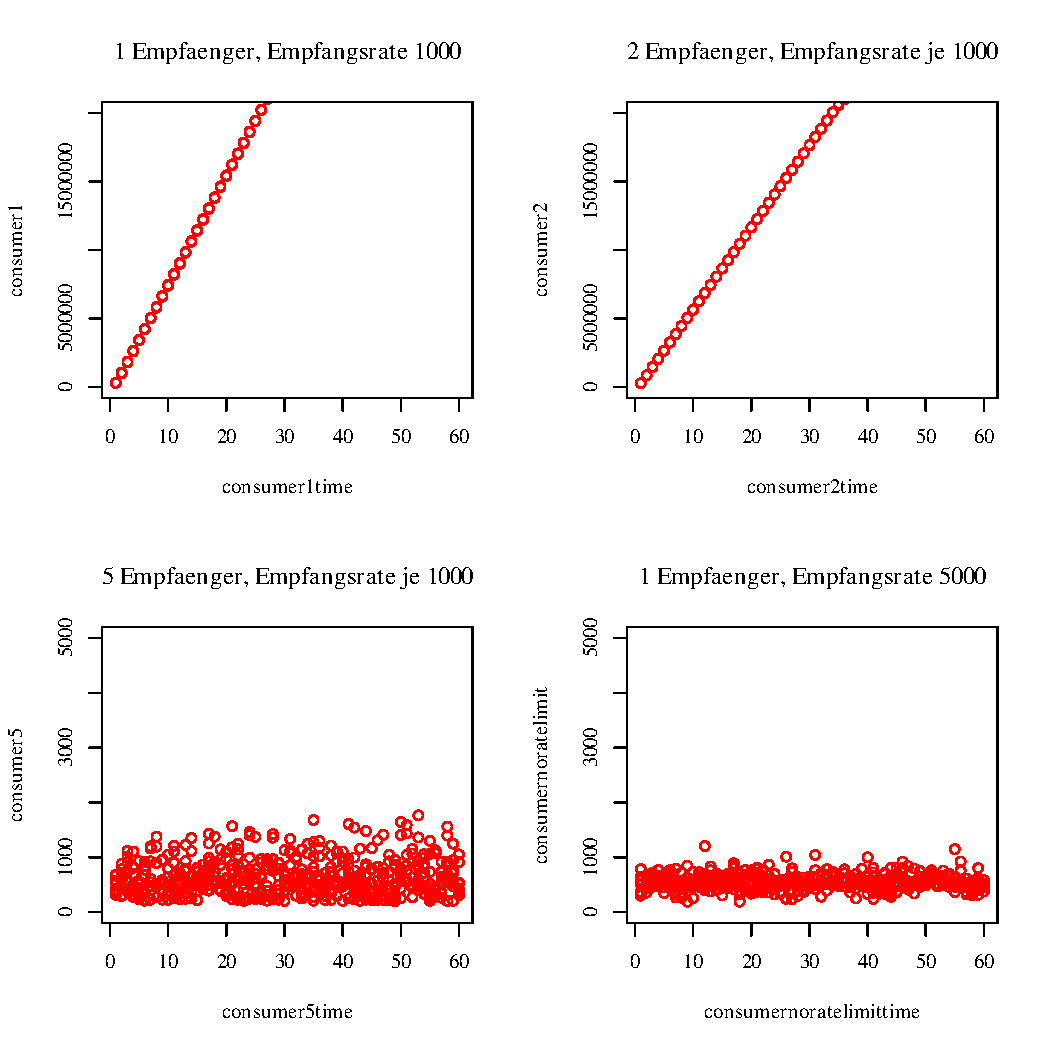
\includegraphics[width=0.7\textwidth]{images/measurement/varying-consumer.pdf}
  \caption{Verschiedene Anzahl an Empfängern mit gleicher Empfangsrate.}
  \label{img:varyingConsumer}
\end{figure}
%E
Diese stärkere Streuung lässt sich mit der Synchronisation der Empfänger erklären, die an einer gemeinsamen Warteschlange arbeiten. Da diese Streuung nicht stark ist, wird dieser Effekt im Folgenden vernachlässigt. Somit zeigt diese Messung, dass mehrere Empfänger gemeinsam an die Leistung eines einzelnen Empfängers heran kommen. 

\subsubsection{Mehrere Sender}
Diese Messung soll überprüfen, ob mehrere Sender genau so schnell die gleiche Menge an Nachrichten versenden können, wie ein einzelner. Dazu wurde als Referenz ein Sender mit einer Senderate von 5000 Nachrichten die Sekunde und fünf Sender mit jeweils 1000 Nachrichten die Sekunde untersucht. Die Messung wurde mit dem \textit{lokalen}-Szenario durchgeführt. Erwartet wird, dass es keinen Unterschied macht, ob ein Sender 5000 Nachrichten sendet oder fünf Sender jeweils 1000 Nachrichten senden. 
%B
In \autoref{img:varyingProducer} sind die Ergebnisse dieser Messung zu sehen. Dabei ist zu sehen, dass mehr Sender etwas schlechter abschneiden als ein einzelner. 
\begin{figure}
\center
  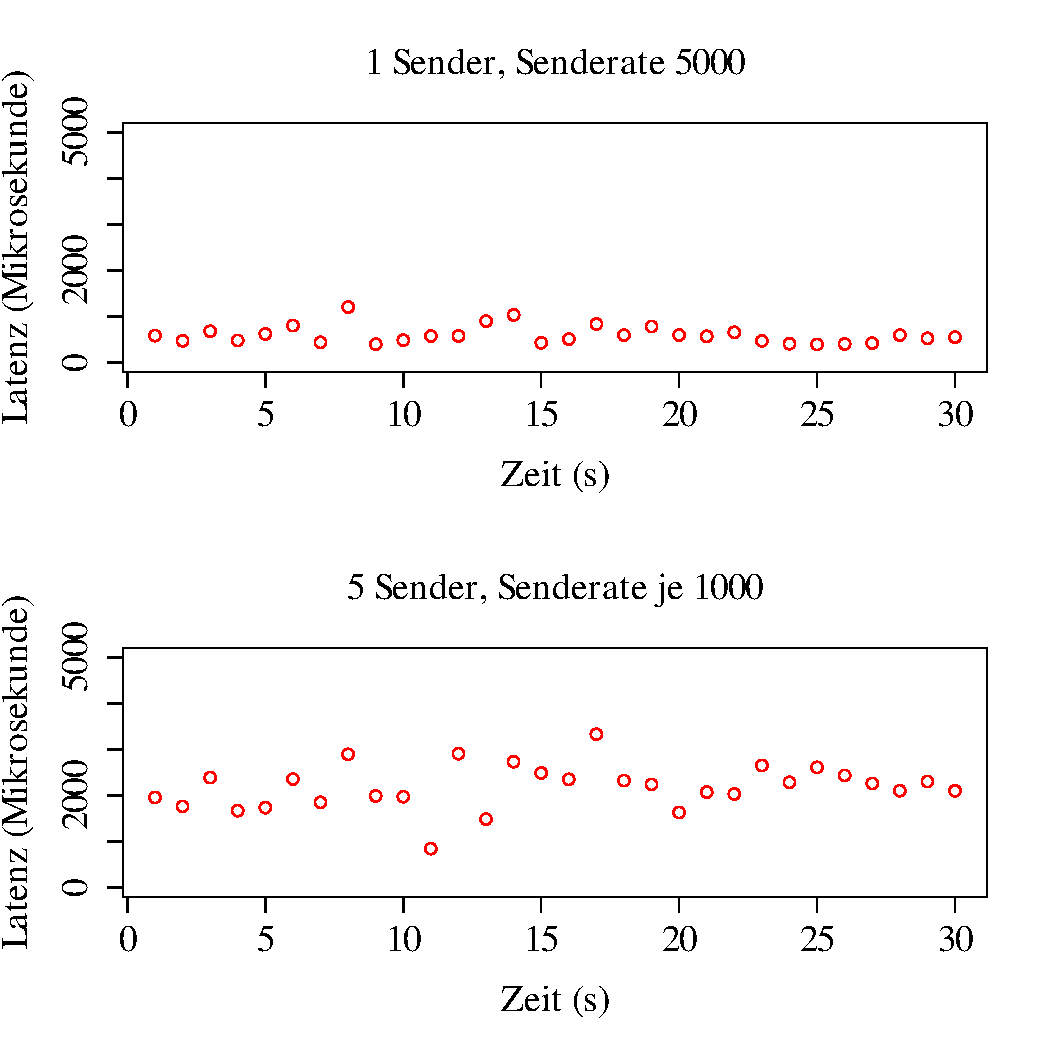
\includegraphics[width=0.7\textwidth]{images/measurement/varying-producer.pdf}
  \caption{Verschiedene Anzahl an Sendern mit gleicher Senderate.}
  \label{img:varyingProducer}
\end{figure}
%E
Auch in diesem Fall kann die höhere Latenz, der mehreren Sender, auf die Synchronisation an einer Warteschlange zurückgeführt werden. Da jedoch dieser Effekt wieder im Mikrosekunden Bereich ist, wird dieser Effekt im Folgenden für die Modellierung vernachlässigt. 
%A
%In einer weiteren Messung sollte Ausserdem geprueft werden, ob mehrere Sender ohne Sendelimit mehr Nachrichten senden koennen als ein Sender. Dazu wurde der selbe Versuchsaufbau wie oben gewaehlt mit dem Unterschied, dass diesmal die Senderate nicht eingeschraenk wurde.
%B
%In \autoref{img:varyingProducerMaxThroughput} sind die Ergebnisse dargestellt. Dabei ist zu sehen, dass die 5 Sender zusammen genauso viele Nachrichten senden wie ein Sender allein. Ausserdem ist die Latenz im Fall der 5 Sender um ein 5faches groesser als bei einem Sender.
%\begin{figure}
%\center
%  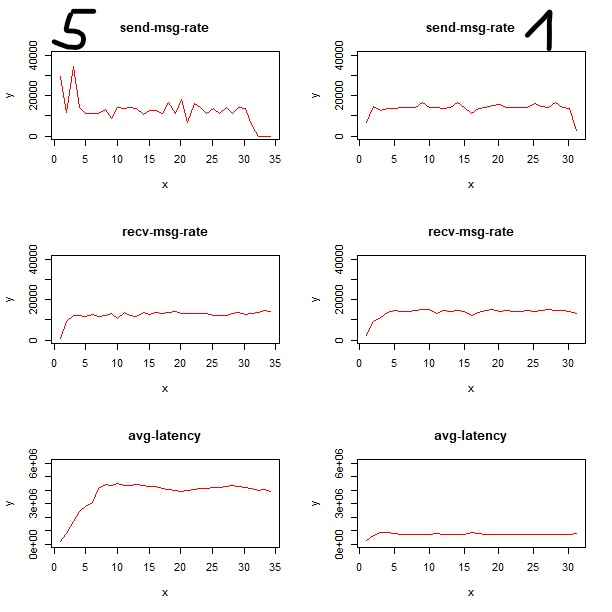
\includegraphics[width=1\textwidth]{images/varyingProducerMaxThroughput.jpg}
%  \caption{Verschiedene Sender Anzahl}
%  \label{img:varyingProducerMaxThroughput}
%\end{figure}
%E
%Das die 5 Sender jeweils nur 1/5 der moeglichen Senderate senden, kann dadurch erklaert werden, dass das Testsystem nicht mehr als eine bestimmte Rate an Nachrichten senden kann. D.h. das es keinen Unterschied macht ob ein Sender oder mehrere Sender Nachrichten senden. DIeses Verhalten kann sich aendern, wenn sich verschiedene Sender auf verschiedenen Maschinen befinden. (evtl noch Messung durchfuehren um zu zeigen) 


%Ableitung von ResourceDemands -> Regressionsfkt

%\subsection{ActiveMQ}
%ActiveMQ \cite{activeMQ} ist eine Open-Source-MOM, die seit 2004 kontinuierlich weiter entwickelt wird. ActiveMQ ist in Java geschrieben und implementiert den Java Message Service (JMS) \cite{jms}. Dabei handelt es sich um eine Programmierschnittstelle zur Ansteuerung einer MOM. Dabei soll eine lose gekoppelte, verlässliche und asynchrone Kommunikation zwischen den Komponenten einer verteilten Anwendung ermöglicht werden. ActiveMQ verfügt außerdem über mehrere Betriebsarten für hohe Verfügbarkeit und einen robusten horizontalen Skalierungsmechanismus. Darüber hinaus ist es sehr flexibel in der Konfiguration und unterstützt eine Vielzahl von Transportprotokollen, darunter auch AMQP.

\subsection{Zusammenfassung}
\label{sec:rmqZusammenfassung}
Mithilfe der durchgeführten Messungen konnten die folgenden Einflussfaktoren identifiziert werden, die einen Einfluss auf die Performance haben:
\begin{itemize}
    \item Die Nachrichtengröße hat einen Einfluss auf die Latenz einer Nachricht, die mögliche Senderate und den Datendurchsatz.
    \item Die Netzwerklatenz zwischen Sender, Empfänger und RMQ hat einen zusätzlichen Einfluss auf die Latenz einzelner Nachrichten.
    \item Der Datendurchsatz, ist durch die Netzwerkverbindung begrenzt.
    \item Wenn Nachrichten direkt aus der Warteschlange empfangen werden können, ist ihre Latenz gering.
    \item Die Latenz der Nachricht steigt, wenn die Warteschlange sich füllt und die Nachrichten in ihr warten müssen um abgeholt zu werden.
    \item Das Begrenzen der Warteschlangengröße kann die Latenz der Nachrichten klein halten.
    \item Ob Nachrichten in den Hauptspeicher oder auf die Festplatte geschrieben werden hat einen Einfluss auf die Latenz (persistente Nachrichten und Lazy-Warteschlangen).
\end{itemize}
Mithilfe dieser Einflussfaktoren soll im Folgenden ein Modell einer MOM erstellt werden, mit dem diese Einflussfaktoren abgebildet werden können. Außerdem werden die Messergebnisse dieses Kapitels verwendet um das Modell zu kalibrieren.


%RMQ hat auch Prefetch von Nachrichten. Wird nicht betrachtet (zeit und trotzdem nicht so gut wie kafka) \\
%Latenz steigt an, wenn die queue gefuellt wird \\
%- benoetigt tracken einer Nachricht durch das system \\
%- explizite Queue Modellierung, mit groesse und fuellstand \\


%--	Vergleich: https://stackshare.io/stackups/activemq-vs-kafka-vs-rabbitmq  \\



%% LaTeX2e class for student theses
%% sections/evaluation.tex
%% 
%% Karlsruhe Institute of Technology
%% Institute for Program Structures and Data Organization
%% Chair for Software Design and Quality (SDQ)
%%
%% Dr.-Ing. Erik Burger
%% burger@kit.edu
%%
%% Version 1.3.3, 2018-04-17

\chapter{Modellierung}
\label{ch:modellierung}
Wie bereits in \autoref{sec:eventbasetransformation} beschrieben bietet das PCM die Möglichkeit eventbasierte Kommunikation zu modellieren und auch eine konkrete MOM Architektur zu modellieren, die mithilfe einer Modelltransformation in die Systemarchitektur eingewoben wird. Diese Modellierung hat jedoch das Problem, dass die Kommunikation nur in eine Richtung funktioniert, wie in \autoref{img:oldEventBased}a zu sehen. Ein Sender sendet eine Nachricht an einen Empfänger und auf dem Weg dorthin durchläuft die Nachricht eine Komponentenkette und wird mit bestimmten Ressourcenanforderungen belegt. Der Empfänger erhält schließlich die Nachricht. In diesem Szenario fehlt jedoch die Warteschlange, die eine wichtige Komponente einer MOM ist. Eigentlich sollte die Komunikation wie in \autoref{img:oldEventBased}b abgebildet stattfinden. Der Sender sendet die Nachricht an die MOM, diese leitet die Nachricht an die entsprechende Warteschlange weiter und ein Empfänger holt sich die Nachricht ab, sobald er die Ressourcen dazu hat. Dieses Szenario ist mit der aktuellen eventbasierten Kommunikation in PCM nicht darstellbar, weil kein abholen einer Nachricht vorgesehen ist. Deshalb soll im Folgenden eine Modellierung präsentiert werden, die eine explizite Warteschlange und ein Verteilsystem, das Nachrichten an passenden Warteschlangen verteilt, modelliert.\par
Dazu soll zunächst mithilfe einer Anforderungserhebung in \autoref{sec:anforderungserhebung} Anforderungen gesammelt werden, die eine solche Modellierung erfüllen soll. Im Anschluss wird in \autoref{sec:modell} die Modellierung einer MOM vorgestellt, die die Anforderungen erfüllen soll. In \autoref{sec:modellkalibrierung} soll das Modell mithilfe der in \autoref{sec:rmqBenchmark} ausgemessenen MOM RMQ kalibriert werden. Dabei soll ein kalibrierter MOM Baustein entstehen, der sich wie die ausgemessene MOM verhalten soll. Schließlich wird in \autoref{sec:momsimulation} das MOM Modell in mehreren Simulationen eingesetzt werden und mit den realem Messungen verglichen. 
\begin{figure}
\center
  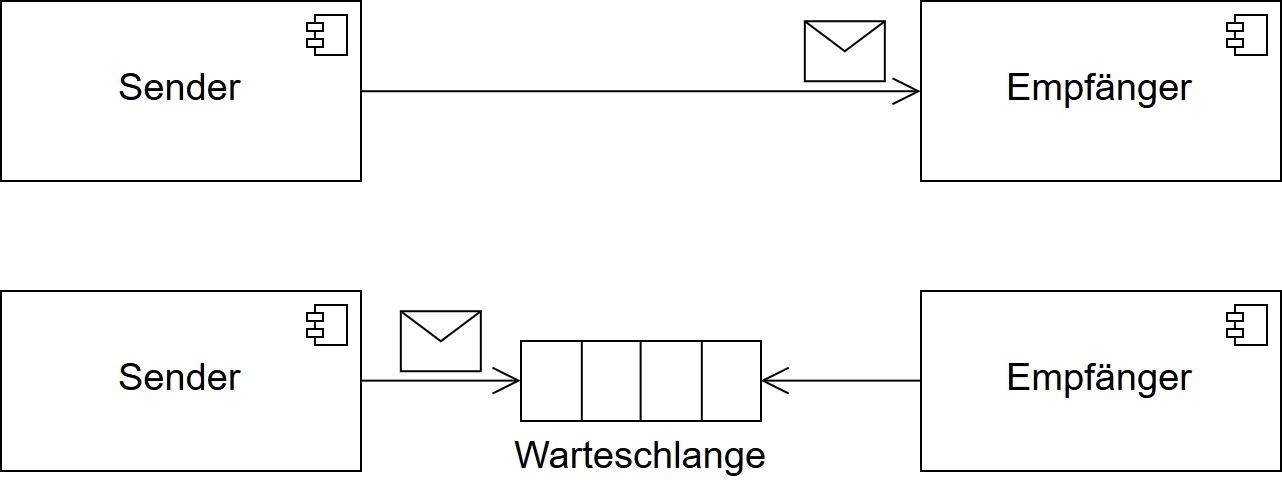
\includegraphics[width=1\textwidth]{images/modelling/oldEventBased.png}
  \caption{Aktuelle eventbasierte Kommunikation}
  \label{img:oldEventBased}
\end{figure}


\section{Anforderungserhebung}
\label{sec:anforderungserhebung}
Aus der Definition einer MOM (siehe Grundlagen) und den Messungen aus \autoref{ch:mom} wurden die folgenden Anforderungen an eine Modellierung abgeleitet. Dabei wurde unterschieden zwischen technischen Anforderungen, also was die Modellierung leisten muss und Anforderungen an die Nutzbarkeit unterschieden. 
Zu den technischen Anforderungen gehören:
\begin{itemize}
    \item Die Modellierung soll das allgemeine Verhalten einer MOM abbilden können.
    \item Asynchrones senden und empfangen von Nachrichten.
    \item Es soll möglich sein eine Nachricht an eine bestimmte Warteschlange oder Topic senden zu können.
    \item Der Füllstand der Warteschlange soll mithilfe der Performanzanalyse ermittelt werden können.
    \item Die Latenz einer Nachricht soll mithilfe der Performanzanalyse ermittelt werden können.
\end{itemize}
Der Benutzer der Modellierung muss in der Lage sein die Folgenden Dinge angeben zu können:
\begin{itemize}
    \item Die Nachrichtengröße muss definierbar sein
    \item Die Topic einer Nachricht muss definierbar sein
    \item Die Anzahl der Nachrichten die pro Sekunde gesendet werden muss angegeben werde können
\end{itemize}

%Angabe des Durchsatzes \\


%Das Ziel ist es eine allgemeine MOM Modellierung zu erstellen, die das Verhalten einer MOM abbilden kann. Dabei soll nicht Wert auf ein spezielles Verhalten gelegt werden. Stattdessen soll es moeglich sein die Modellierung um Konfigurationen, wie zum Beispiel RMQs lazy Queues, erweitern zu koennen. 

\section{Modell}
Im Folgenden soll eine Modellierung einer MOM präsentiert werden die die zuvor definierten Anforderungen erfüllt. Dabei war nicht das Ziel eine Meta-Modell Erweiterung zu erstellen, sondern mit bereits existierenden PCM-Elementen zu arbeiten. 

%Anhand der bekannten MOM Architekturen aus der Untersuchung verschiedener MOMs wurde versucht zu definieren wie eine MOM modelliert werden kann. Dabei wurden die Anforderungen versucht umzusetzen. \\
%- 2 Moeglichkeiten entweder mit oder ohne Exchange explizit zu modellieren.\\
%- Vorteil Explizit: RDs fuer verteilung (konnte aber nicht ausgemessen werden) \\
%- Nachrichten Typen mitschicken (fanout, direct) und in Branches auswerten

\subsection{Repository}
Das Repository wird vom Komponentenentwickler verwendet um neue Komponenten zu erstellen und vom Systemarchitekt um Komponenten zu entnehmen. ... \\
Die untersuchte MOM Architektur besteht aus einem Verteiler und einer Warteschlange. Deshalb wurdem die in \autoref{img:mom_repository} abgebildeten Komponenten und Schnittstellen definiert. Die Schnittstelle nach ausen soll die IExchange Schnittstelle sein. Diese bietet zwei Signaturen an. Eine zum Empfange (receive) und eine zum Senden (distribute) einer Nachricht. Beide Methoden werden von der Komponente Exchange angeboten. IQueue ist die zweite Schnittstelle. Diese bietet auch zwei Signaturen an. Eine um eine Nachricht in eine Warteschlange abzulegen (put) und eine weitere die eine Nachricht aus der Warteschlange entnimmt (get). Diese Schnittstelle wird von der Komponente Queue angeboten. Diese Komponenten, die eine Warteschlange abbildeen soll, besitzt eine Passive Resource die das Verhalten einer Warteschlange simulieren soll. Eine Passive Ressouce ist... (TODO). Dabei wird das ablegen in die Warteschlange als release auf die passive Ressource und das entnehmen aus der Warteschlange als aquire auf die passive Ressource modelliert. Die Exchange Komponente benötigt eine Komponente die die IQueue Schnittstelle anbietet. Die Idee ist, dass alle Warteschlangen die benötigt werden von der Exchange Komponente required werden. In \autoref{img:mom_repository} sind das aktuell zwei Warteschlange. Mithilfe des RDSEFFs kann die Exchange Komponente zwischen den Warteschlangen wechseln. Dies ist in \autoref{img:queueBranch} dargestellt. Dabei wird mithilfe eines GuardedBranch geprüft an welche Warteschlange die ankommenden Nachricht gehen soll. Der Fall, dass eine Nachricht aus der Warteschlange entnommen wird funktioniert genauso. 


%Dieser Ansatz ermöglicht es jedoch nicht einzelne Nachrichten durch das System zu verfolgen. \\


\begin{figure}
\center
  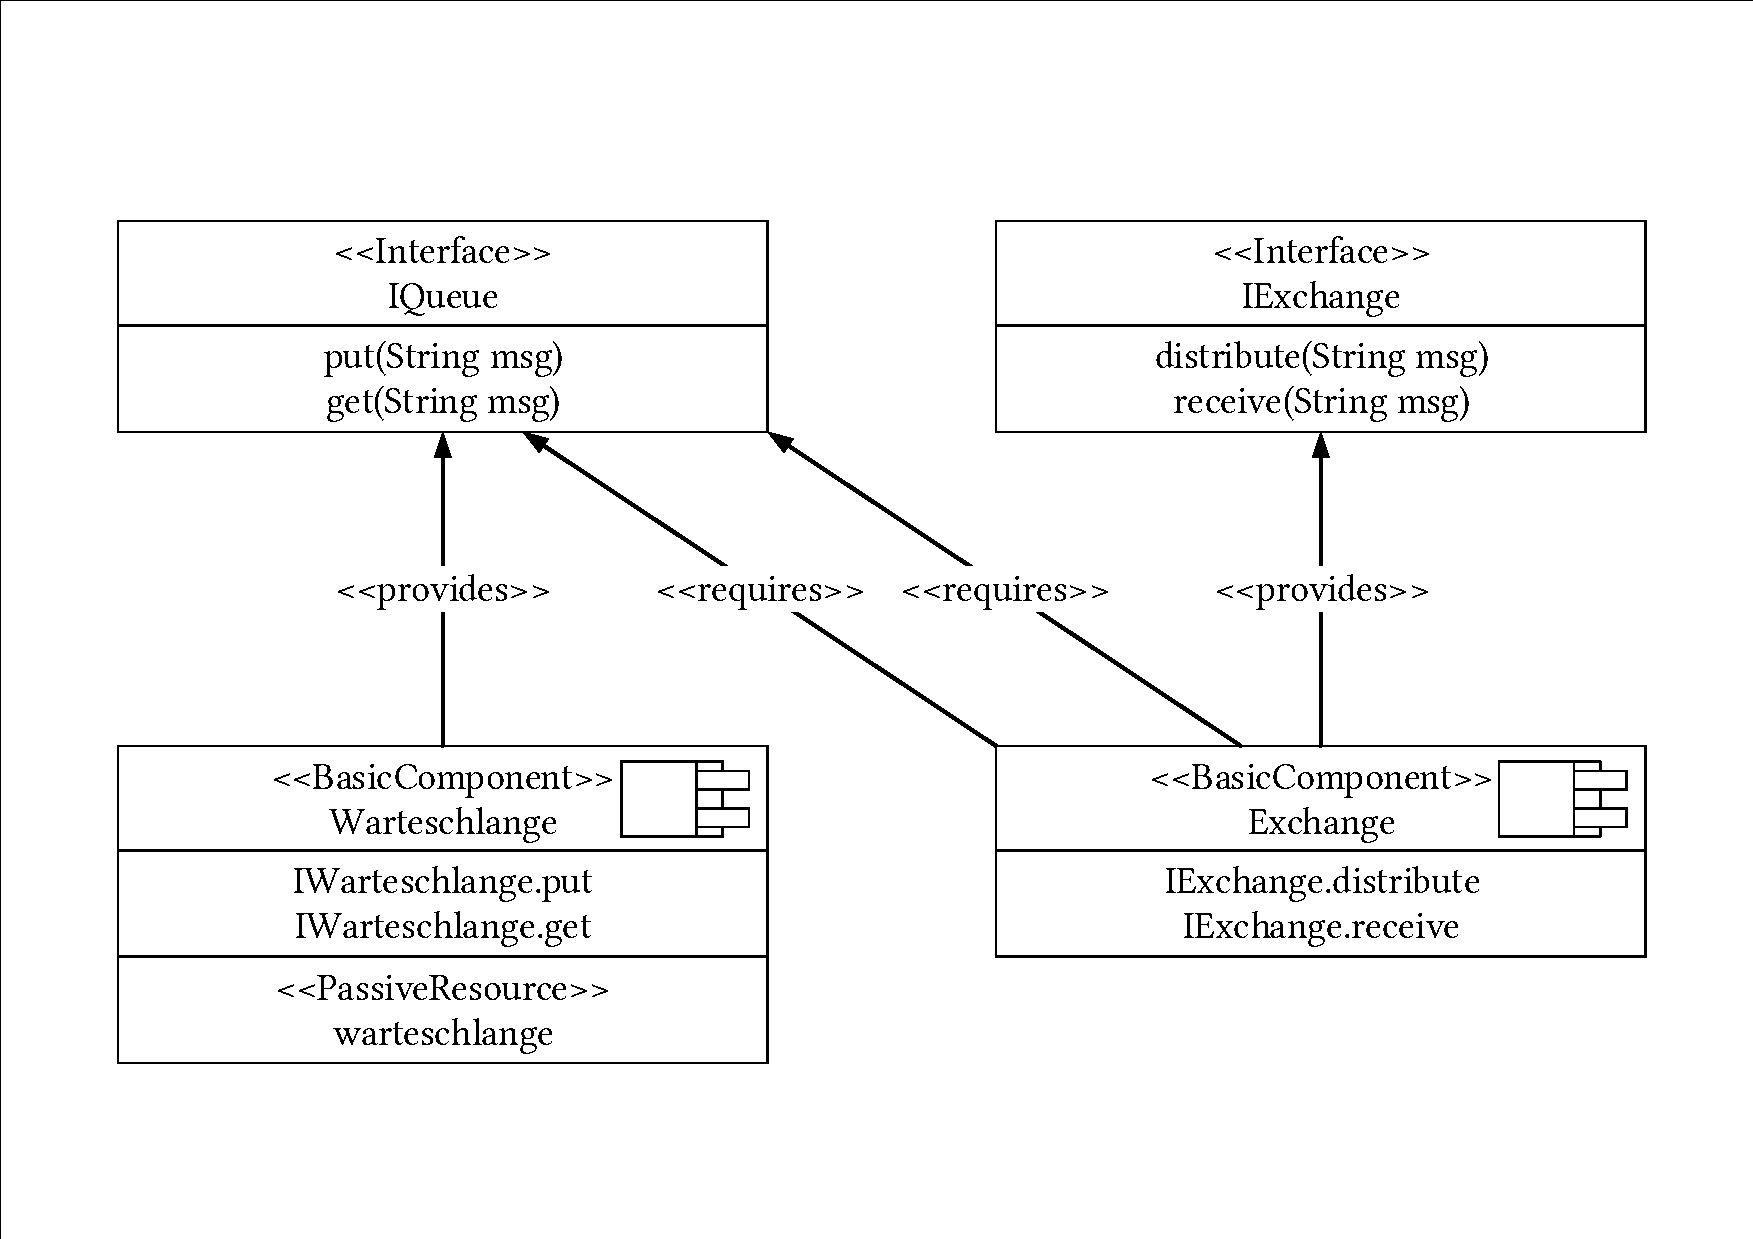
\includegraphics[width=1\textwidth]{images/modelling/repository.pdf}
  \caption{Repository einer MOM mit Exchange und Warteschlange}
  \label{img:mom_repository}
\end{figure}

\begin{figure}
\center
  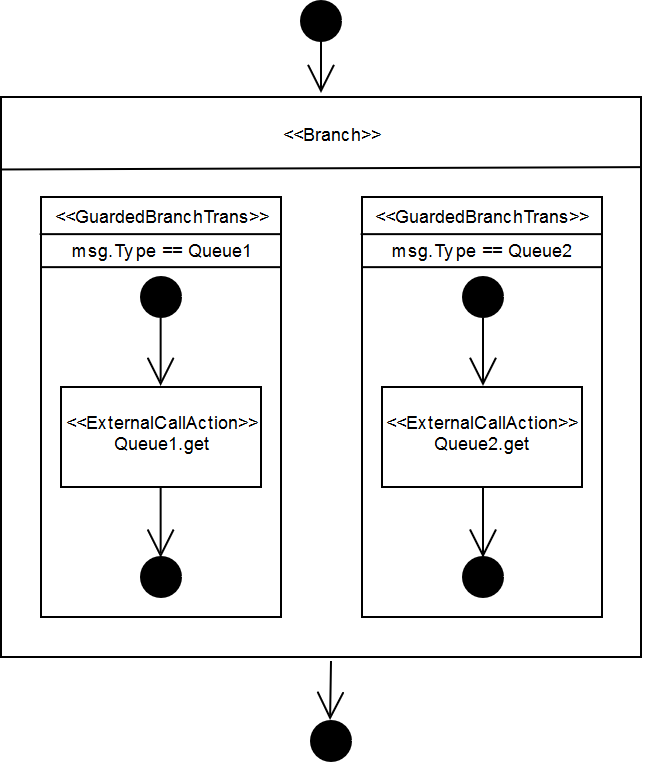
\includegraphics[width=0.7\textwidth]{images/modelling/branchSeff.png}
  \caption{Repository einer MOM mit Exchange und Warteschlange}
  \label{img:queueBranch}
\end{figure}

\subsection{System}
Im Systemmodell werden die einzelnen Komponenten aus dem Repository vom Softwarearchitekten zu einem System zusammengesetzt. Der Software-Architekt kann nun die Komponenten aus dem zuvor definierten Repository zusammensetzen. Dabei kann er zunächst entscheiden, wie viele Exchange Komponenten im System exisitieren sollen. Wie auch in RMQ kann eine MOM aus mehreren Exchanges bestehen, die sich auf unterschiedlichen Maschinen befinden können. An einen Exchange werden dann die dazugehörigen Warteschlangen angeschlossen. Da ein Exchange eine Schnittstell zum Senden und Empfangen von Nachrichten anbietet, können beliebig viele Sender und Empfänger Komponenten an einen Exchange angeschlossen werden. In \autoref{img:mom_system} ist ein Systemmodell mit zwei Exchange Komponenten abgebildet. Dabei hat Exchange1 zwei Warteschlangen Komponenten und Exchange2 nur eine Warteschlange angeschlossen. Außerdem sind an Exchange1 je ein Sender und Empfänger angeschlossen. An Exchange2 sind zwei Sender und ein Empfänger angeschlossen. 

\begin{figure}
\center
  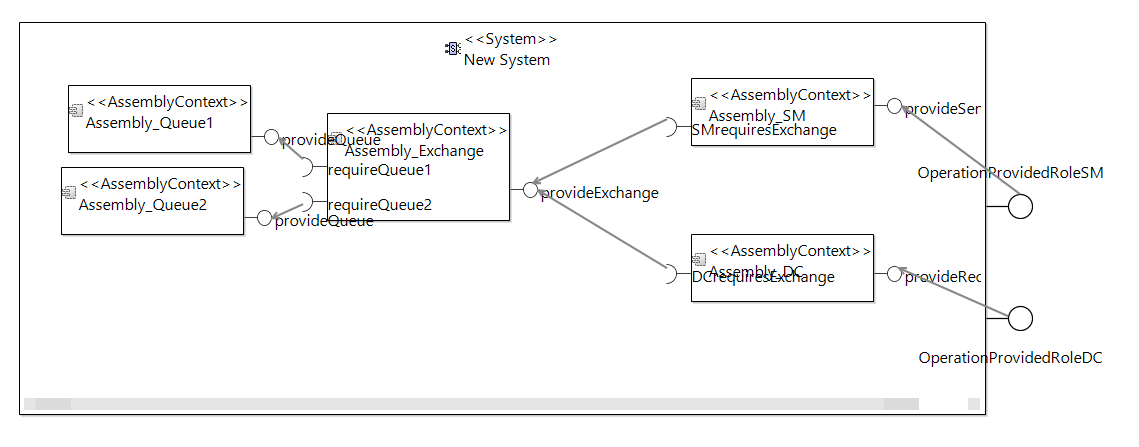
\includegraphics[width=1\textwidth]{images/mom_system.png}
  \caption{Systemmodell einer MOM}
  \label{img:mom_system}
\end{figure}
\subsection{Ausführungsumgebung und Allokation}
Im Ausführungs-Umgebungs-Modell kann der Software-Verteilungs-Experte die Hardware Knoten und Netzwerkverbindungen darstellen. Für jeden Exchange und jede Warteschlange kann eine eigene Ressource definiert werden. Außerdem müssen die einzelnen Verbindungen zwischen einem Exchange und den Sendern und Empfängern modelliert werden. Falls Exchange und Warteschlange sich auf unterschiedlichen Ressourcen befinden, müssen die Verbindungen auch modelliert werden. In \autoref{img:mom_ressorceEnv} ist eine mögliche Ausführungsumgebung für das oben beschriebene System dargestellt. Die Ausführungsumgebung besteht aus je einer MOM Ressource für den jeweiligen Exchange und die an ihn angeschlossenen Warteschlangen. Die einzelnen Sender und Empfänger sind jeweils auf eigenen Ressourcen verteilt und sind über Netzwerkverbindungen mit der jeweiligen MOM Ressource verbungen. 
\begin{figure}
\center
  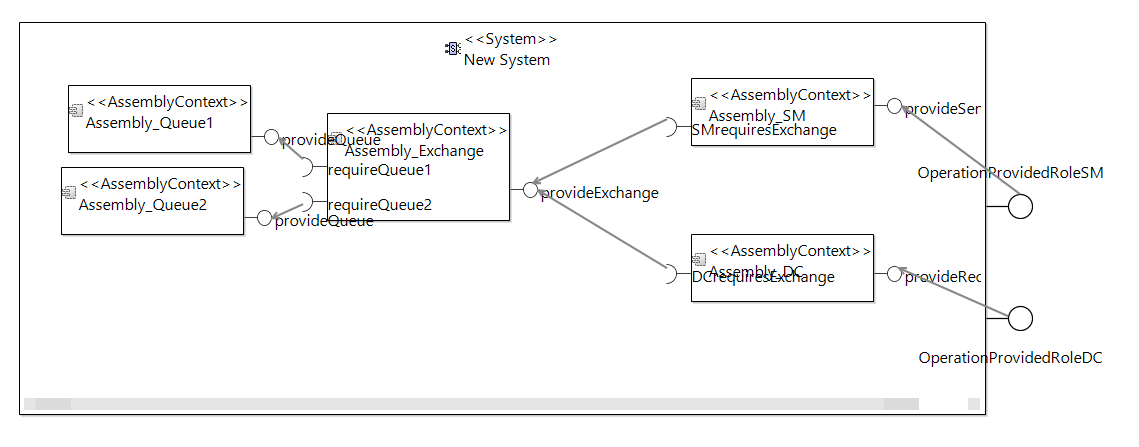
\includegraphics[width=1\textwidth]{images/mom_system.png}
  \caption{Ausführungsumgebung und Allokation einer MOM}
  \label{img:mom_ressorceEnv}
\end{figure}

\subsection{Nutzungsmodell}
Im Nutzungsmodell wird die Benutzung des Systems durch den Domänenexperten modelliert. Für jeden Sender und Empfänger wird dazu je ein UsageScenario angelegt. Dieses beinhaltet das Verhalten eines Benutzers und seine Ankunftszeit. Der Domänenexperte kann somit festlegen wie oft ein Sender oder Empfänger pro Zeiteinheit ankommt um Nachrichten zu senden oder zu empfangen. Außerdem kann dadurch die Anzahl der Nachrichten die pro Zeiteinheit gesendet werden abgebildet werden. Wenn ein Sender zum Beispiel 0.1 mal pro Zeiteinheit ankommt, heißt das, dass er 10 mal pro Zeiteinheit ankommt und somit 10 Nachrichten versendet. Neben der Ankunftzeit wird im UsageScenario auch das Verhalten modelliert. Mithilfe eines EntryLevelSystemCalls kann die passende Funktion im passenden Exchange aufgerufen werden. Möchte ein Sender ein Nachricht an einen Exchange senden, muss er mithilfe des ELSC den passenden Exchange auswählen. Mithilfe von UsageVariablen, könnne dem Aufruf außderdem Parameter mitgegeben werden. Mithilfe dieses Mechanismuses kann für jeden Aufruf spezifiziert werden wie groß die Nachricht die gesendet oder empfangen werden soll ist und zu welcher Warteschlange oder Topic sie gehört. In \autoref{img:mom_usage} ist ein mögliches Nutzungsmodell für das oben beschriebene System. Dabei wird nur der Teil mit Exchange1 betrachtet. Das Nutzungsmodell besteht aus zwei UsageScenarios. Das erste stellt den Sender des Systems dar. Seine Interaktion mit dem System besteht darin, die distribute Funktion im Exchange1 aufzurufen und dabei eine Nachricht mit 5000 Bytes zu versende. Da seine Ankuftszeit 0.1 Beträgt, tut er die zehn mal pro Zeiteinheit. Das zweite UsageScenario stellt den Empfänger des Systems dar. Seine Interaktion mit dem System besteht darin, die receive Funktion im Exchange1 aufzurufen und dabei eine Nachricht mit 5000 Bytes zu empfangen. Da seine Ankuftszeit 0.5 beträgt, tut er die fünf mal pro Zeiteinheit. Da der Empfänger somit pro Zeiteinheit fünf der zehn Nachrichten nicht empfängt sollten diese in der Warteschlange landen und in einer Simulation sichtbar.
\begin{figure}
\center
  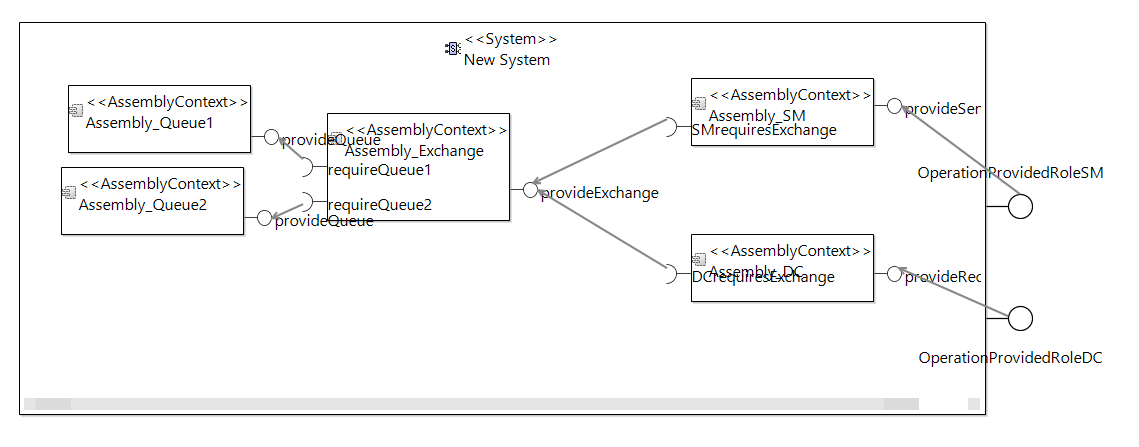
\includegraphics[width=1\textwidth]{images/mom_system.png}
  \caption{Nutzungsmodell einer MOM mit einem Sender und Empfänger}
  \label{img:mom_usage}
\end{figure}

\section{Modellkalibrierung}
\label{sec:rmqRd}
In \cite{palladio17} wird Modellkalibrierung als Anreicherung von Modellen mit quantitaitven Daten, wie Ressourcenbedarf. Je nachdem wie weit entwickelt das System ist, können diese Daten mithilfe von verschiedenen Techniken gewonnen werden. Mithilfe von Application-Performance-Monitoring wurde in \autoref{sec:rmqBenchmark} RMQ ausgemessen und die Ergbnisse dort beschrieben. Im Folgenden sollen die Ergebnisse interpretiert und benutzt werden um die Modelle zu kalibrieren.
%Das Ziel ist, dass der Benutzer keinen MOM spezifischen RD angeben muss. \\

In \autoref{oneMsgLatency} wurde die Latenz einer Nachricht mit verschiedenen Größen ausgemessen. Darin ist ein lineares Wachstum der Latenz mit ansteigen der Nachrichtengröße zu beobachten. Dies liegt die Vermutung nahe, dass diese beiden Variablen voneinander abhängen. Um diese Vermutung zu bestätigen wurde für die Variablen Latenz und Nachrichtengröße ihre Korellation berechnet. Dabei ist die Korrelation ein statistisches Maß, das den Grad der linearen Abhängigkeit zwischen zwei Variablen anzeigt, die im Paar auftreten. Ist diese Abhängigkeit hoch, liegt der Wert nahe eins. Liegt der Wert dagegen bei minus eins, ist die Abhängigkeit sehr gering. Die Korrelation der Variablen Latenz und Nachrichtengröße ist 0.9850627. Somit ist eine hohe lineare Abhängigkeit der Variablen gezeigt. Als nächstes soll mithilfe einer linearen Regressionsanalyse einen Ressourcenbedarf für das Modell definiert werden. Das Ziel einer linearen Regressionsanalyse ist es, eine lineare Beziehung zwischen einer Prädiktorvariable Y und der Reaktionsvariable X herzustellen, so dass der Wert von Y getschätzt werden kann, wenn nur der Wert des Prädiktoren X bekannt ist. Die Ergebnisse sind in \autoref{img:reganalysesummary} und die dabei entstandene Regressionsgerade in (abb) abgebildet. TODO was soll alles rein?
Daraus folgt ein Term der Form: Latenz = 1256.2782902 + (0.003299 * Nachrichtengröße). Dieser Term soll nun als Ressourcenbedarf einer Nachricht dienen, sobald diese aus der Warteschlange entnommen wird. 
\begin{figure}
\center
  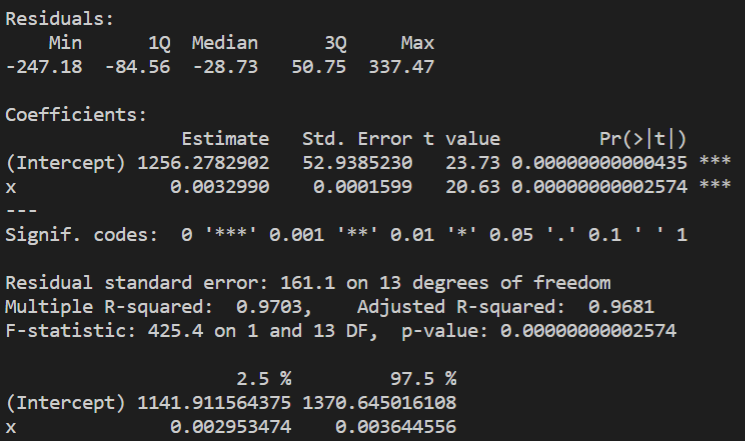
\includegraphics[width=1\textwidth]{images/modelling/reganalyse.png}
  \caption{Ergebniss der Regressionsanalyse}
  \label{img:reganalysesummary}
\end{figure}

\par

In \autoref{sec:maxthroughput} wurde gemessen, was die möglichen Datenmengen sind, die in dem System gesendet werden können. Dabei wurde eine Messung mit und ohne Empfänger durchgeführt. Der Maximalwert aus der Messung ohne Empfänger wird in die LinkingRessources zwischen dem MOM-RessourceContainer und dem Sender und der Maximalwert aus der Messung mit Empfänger wird in die LinkingRessources zwischen dem MOM-RessourceContainer und dem Empfänger jeweils als Throughput eingetragen. Sobald eine Nachricht über diese Verbindung gesendet wird, wird die Nachrichtengröße durch den Throughput geteilt und auf die Gesamtlatenz addiert. \par

Auch die Netzwerklatenz, die in \autoref{oneMsgLatency} ausgemessen wurde, hat einen Einfluss auf die Latenz einer Nachricht gehabt. Wenn diese in der Modellierung betrachtet werden soll, kann diese in die jeweiligen LinkingRessource als Netzwerklatenz eingetragen werden. Diese wird auf die Gesamtlatenz einer Nachricht addiert. \par

Neben der Standardkonfiguration wurde auch die Konfiguration für Lazy-Warteschlangen in \autoref{sec:rmqLazy} ausgemessen. Auch hier wurde wie oben beschrieben zunächst die Korrelation der beiden Variablen berechnet. Mit 0.9951195 ist diese ebenfalls sehr hoch. Die Ergebnisse der im Anschluss durchgeführten Regeressionsanalyse sind in  \autoref{img:reganalysesummarylazy} abgebildet. TODO was soll alles rein?
Daraus folgt ein Term der Form: Latenz = 1602.5021193 + (0.0049697 * Nachrichtengröße). Dieser Term soll nun als Ressourcenbedarf einer Nachricht dienen, sobald diese aus der Warteschlange entnommen wird, wenn Lazy-Warteschlangen betrachtet werden sollen.
\begin{figure}
\center
  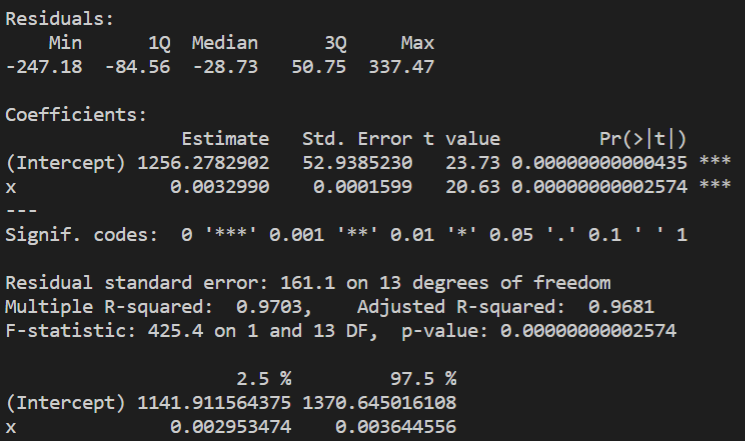
\includegraphics[width=1\textwidth]{images/modelling/reganalyse.png}
  \caption{Ergebniss der Regressionsanalyse}
  \label{img:reganalysesummarylazy}
\end{figure}

Die zuvor beschriebenen Modelle können nun mithilfe der hier vorgestellten quantitativen Daten angereichert werden um eine Performanzanalyse zu ermöglichen. Im nächsten Schritt soll eine konkrete Modellierung vorgestellt werden, die mit den hier vorgestellten Daten angereichert wird. 

%Somit ergibt sich f die Response Time folgendes ergeben: Response Time: ByteSize / Throughput + RD / CPU + Latency + HddRD/HDD \\
%RD an Aquire um Latenz abzubilden

%Als erstes sollte die Sende und Empfangsrate abgebildet werden. Beobachtet man (ref zu Messung verschiedene Senderaten) bemerkt man fuer die ersten Messungen, solange Warteschlange nicht allzu voll wird, einen linearen Anstieg der Latenz. Daraus laesst sich zunaechst folgender RD ableiten:






%Latenz: Unter Latenz versteht man im MOM Kontext, die Zeit, die eine einzelne Nachricht braucht um beim Consumer anzukommen. Da jede Nachricht einen Zeitstempel bekommt kann die Zeit gemessen werden, wenn sie aus der Warteschlange entnommen wurde.

%welche Effekte koennen wir so hoffentlich abbilden

\section{Untersuchung der MOM Modellierung}
In den Abschnitten zuvor wurde vorgestellt wie die Modellierung eines Systems aussehen soll, die eine MOM zum Nachrichtenaustausch verwendet. Im Folgenden wird eine konkrete Modellierung vorgestellt, die mit den quantitativen Daten aus \autoref{} angereichert wird. Anschließend wird eine Performanzanalyse auf der Modellierung ausgeführt. Die Ergebnisse werden anschließend mit den Messungen aus \autoref{sec:rmqBenchmark} verglichen.

\subsection{Anwendungszenario}
Im Folgenden betrachten wir das in \autoref{img:simulationscenario} abgebildete Szenario. Darin befindet sich eine Sender und eine Empfänger Komponente. Beide sind mit der Exchange Komponente verbunden. Der Exchange ist genau mit einer Warteschlange verbunden. Diese ist entweder mit dem RD für eine Nachricht ohne oder mit Lazy-Warteschlangen angereichert. Die Exchange und die Warteschlangen Komponente sind auf einem gemeinsamen ResourceContainer MOM bereitgestellt. Die Sender und Empfänger Komponente sind jeweils auf einem eigenen ResourceContainer bereitgestellt. Der MOM-RC ist jeweils mit dem Sender- und der Empfänger-RC mithilfe einer LinkingResource verbunden. Diese haben jeweils einen Wert für den Durchsatz und Latenz eingetragen, je nachdem welches Szenario betrachtet wird. Schließlich sind für den Sender und Empfänger jeweils ein UsageScenario spezifiziert. Darin sind die jeweiligen Ankunftszeiten und Nachrichtengrößen modelliert.
% Der Sender sendet pro Zeiteinheit und der Empfaenger empfaengt pro Zeiteinheit eine bestimmte Menge an verschieden Großen Nachrichten. 
\begin{figure}
\center
  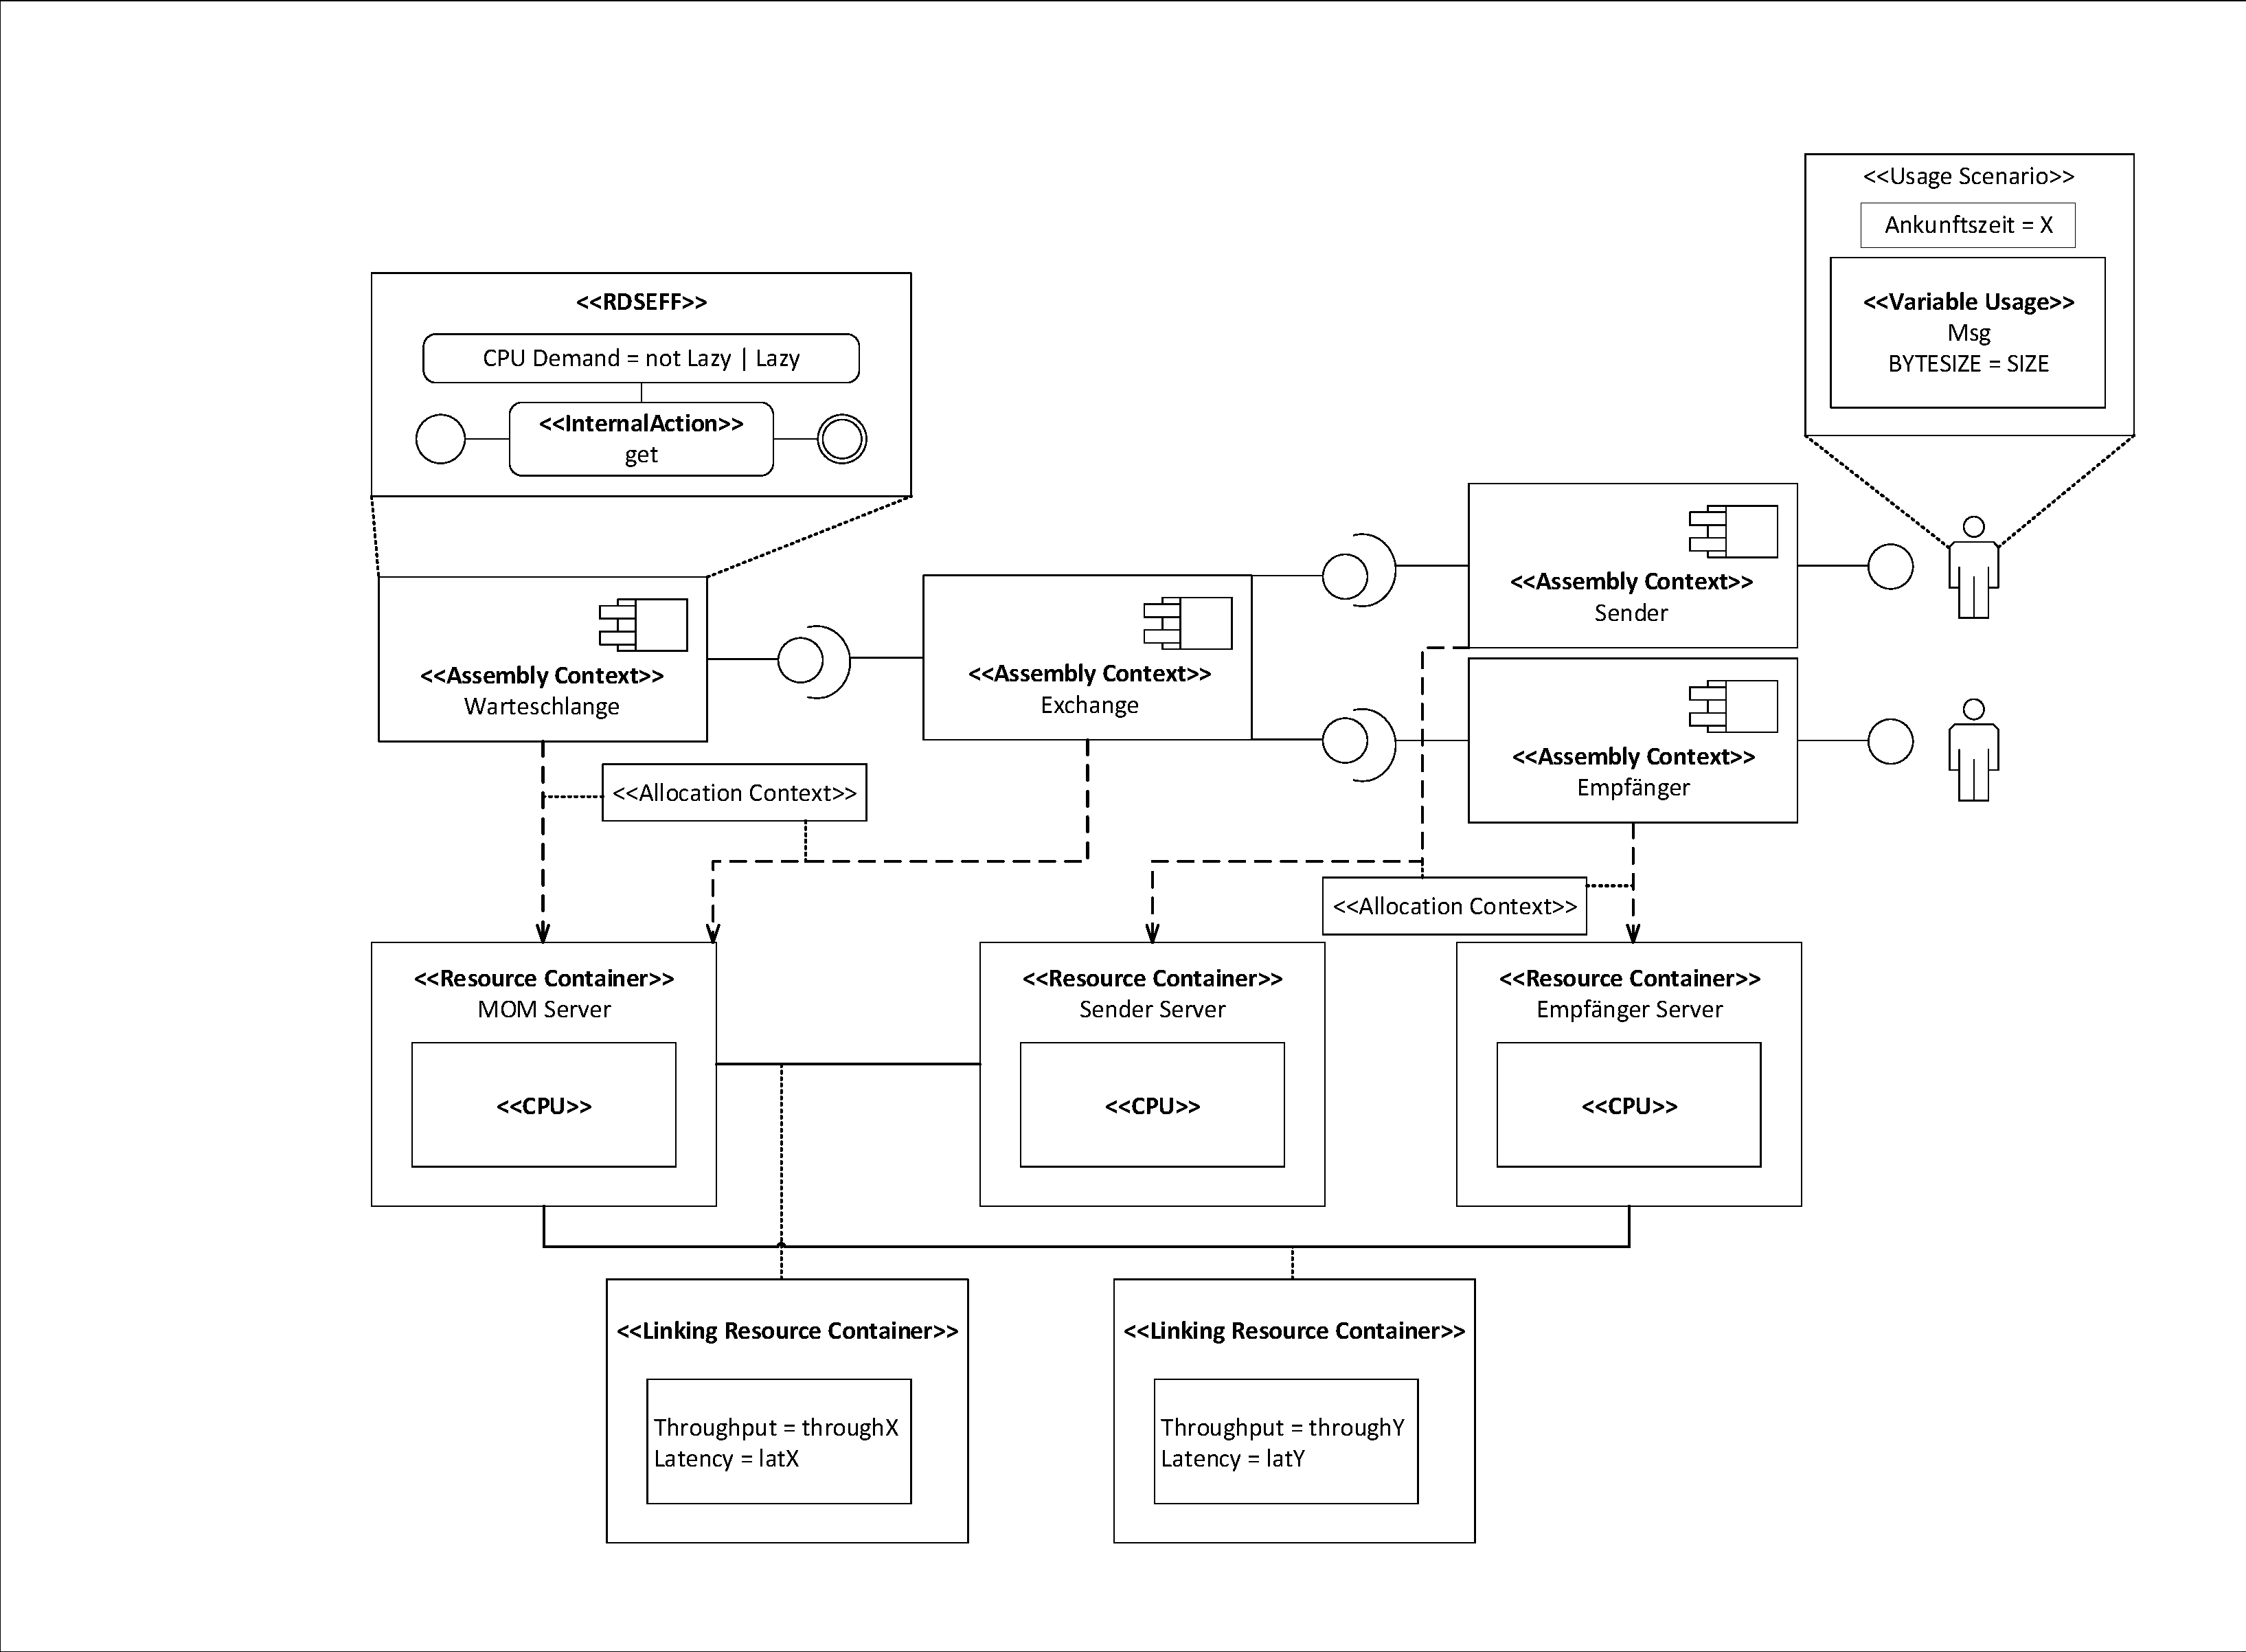
\includegraphics[width=1\textwidth]{images/modelSimulationResults/simulationScenario.pdf}
  \caption{Simulationsszenario }
  \label{img:simulationscenario}
\end{figure}
Im Folgenden wird diese Modellierung in einer Performanzanalyse eingesetzt.


\subsection{Performance-Analyse}
Die Palladio-Bench bietet eine Sammlung von Qualitätsanalysen mit Hauptfokus auf Performance an. Nachdem in den vergangen Abschnitten eine MOM Modellierung und ihre Kalibrierung beschrieben wurde, kann im nächsten Schritt eine Performance-Analyse ausgeführt werden. Dazu wird das Analysewerkzeug \textbf{SimuCom} verwendet, das verschiedene Performance Charakteristiken, darunter Antwortzeiten für Systeme und Komponenten, sowie die Auslastung einzelner Ressourcen berechnet. Im Folgenden werden die Ergebnisse der Performance-Analyse präsentiert und mit den Messungen aus \autoref{sec:rmqBenchmark} verglichen. 
\subsubsection{Simulation 1} 
\label{sec:rmqSimulation1}
In der ersten Simulation wird der Fall betrachtet, dass Sender und Empfänger die gleichen Ankunftszeiten haben. Die gesendete Nachrichten haben die Größen 100, 200, 300, 400, 500 und 1000 Kbyte. Verglichen wurde mit den Messungen aus \autoref{sec:oneMsgLatency}. Der Sender, Empfänger und der Broker befinden sich jeweils auf der selben Maschine. Betrachtet wurden der Füllstand der Warteschlange und die Latenz der Nachrichten. 
%B
Da die Ankunftszeiten der beiden Akteure gleich sind, bleibt die Warteschlange die ganze Zeit über Leer. Die Ergebnisse der Latenz einer Nachricht sind in \autoref{img:simulation1} abgebildet. Eingezeichnet sind dabei die Messpunkte der Messungen und die Ergebnisse der Simulation. In (tabelle) ist der Fehler für jede Größe angegeben. Dabei ist zu sehen, dass dieser zwischen X und Y liegt.

\begin{figure}
\center
  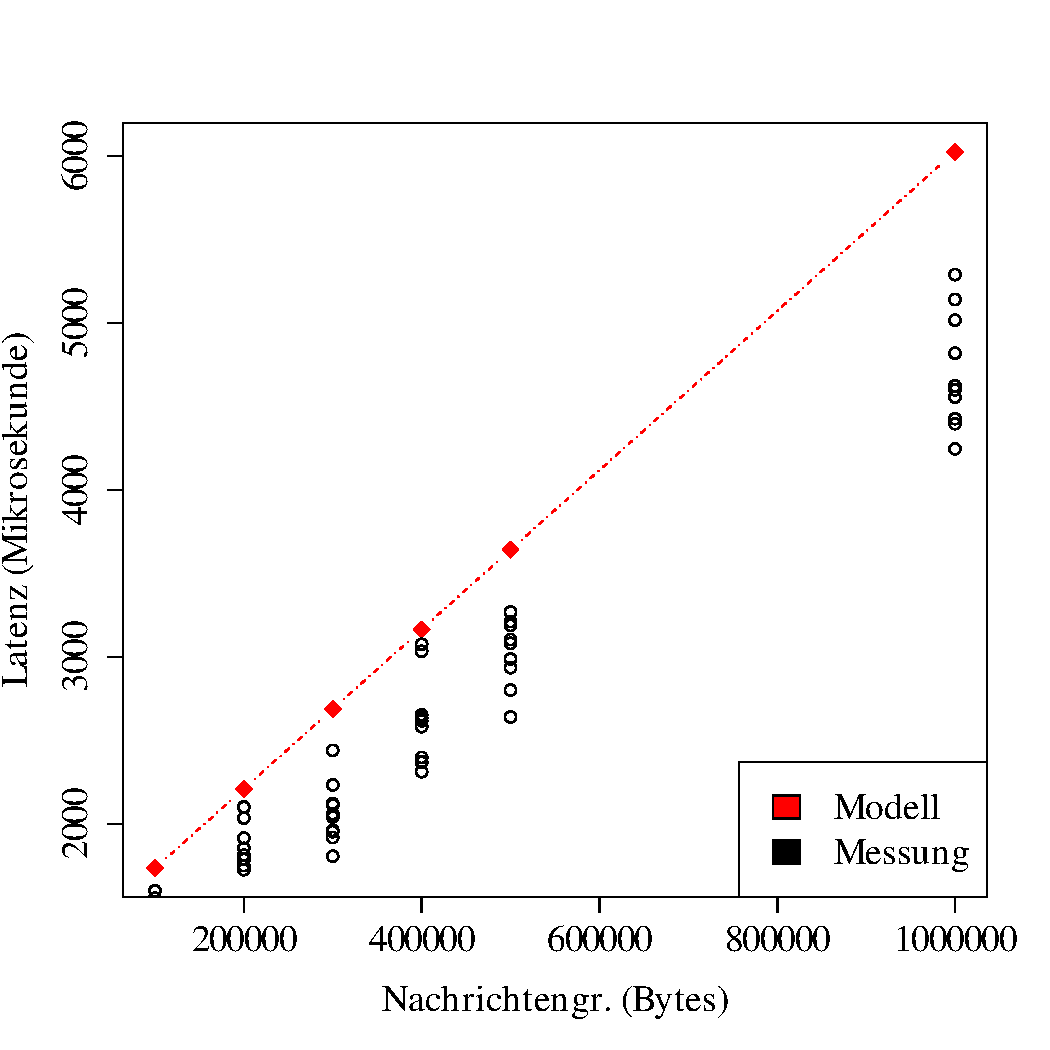
\includegraphics[width=0.5\textwidth]{images/modelSimulationResults/simulation1.pdf}
  \caption{Latenz einer Nachricht mit verschiedenen Groessen (Modell vs. Real System)}
  \label{img:simulation1}
\end{figure}

\subsubsection{Simulation 2} 
Diese Simulation betrachtet zusätzlich zu dem Fall aus Simulation 1 die Netzwerklatenz mit. Dazu sind Sender, Empfänger und Broker auf unterschiedlichen Maschinen. Die Nachrichten haben die größen 100, 200, 300, 400, 500 und 1000 Kbyte. Im Modell wurden für die LinkingRessources der Durchsatz und die Latenz, wie in \autoref{sec:rmqRd} beschrieben, für entfernte Broker angepasst. Die Messung mit der verglichen wurde ist in \autoref{sec:oneMsgLatency} beschrieben. Es wurden der Füllstand der Warteschlange und die Latenz der Nachrichten betrachtet. 
%B
Die Warteschlange bleibt über die Simulationsdauer leer, da die Ankunftszeiten der Sender und Empfänger gleich sind. Die Latenz der Nachrichten ist in \autoref{img:simulation2} abgebildet. Außerdem sind die Messpunkte aus der Messung eingetragen. In (tabelle) ist der Fehler für jede Größe angegeben. Dabei ist zu sehen, dass dieser weniger gut ist, als bei der vorherigen Simulation. Der Fehler liegt zwischen X und Y.
\begin{figure}
\center
  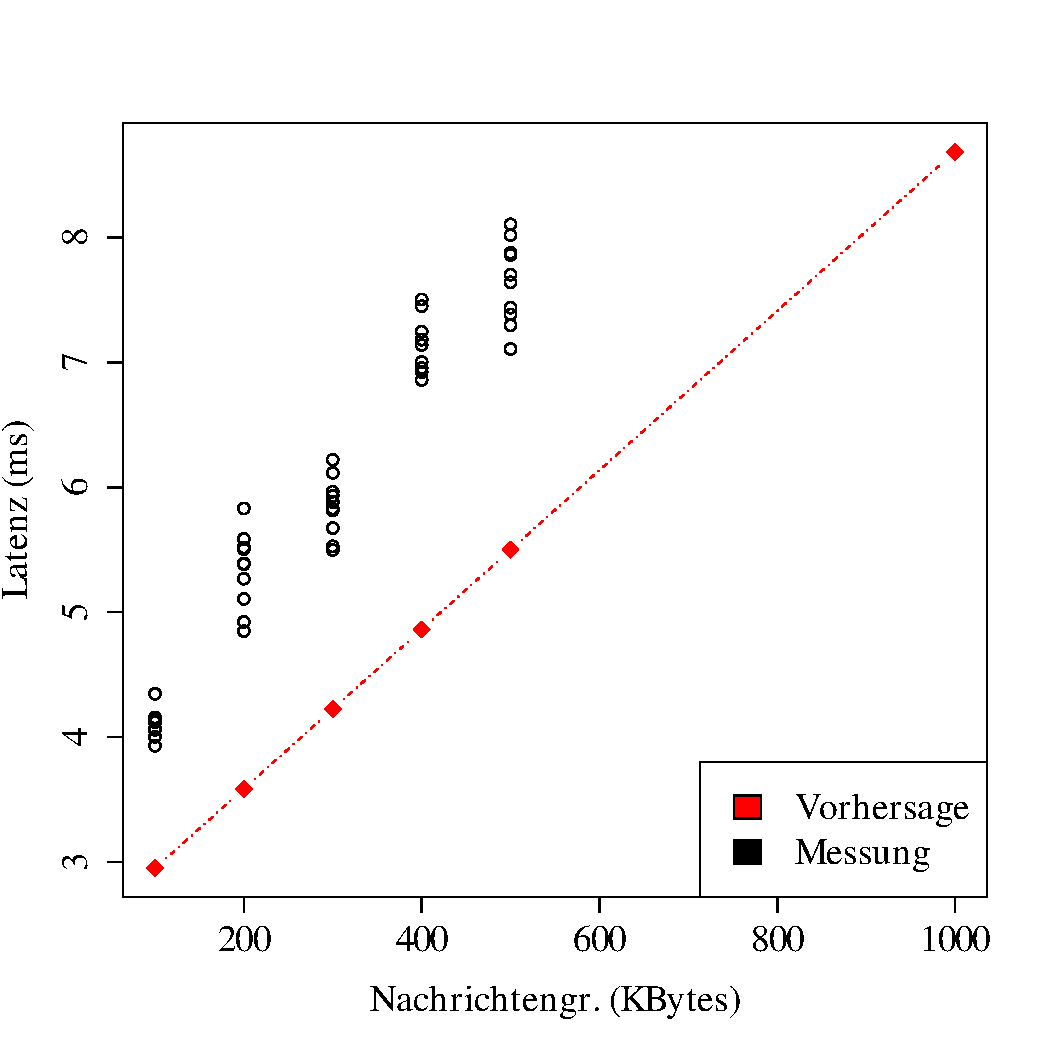
\includegraphics[width=0.5\textwidth]{images/modelSimulationResults/simulation2.pdf}
  \caption{Latenz einer Nachricht mit verschiedenen Groessen mit Netzwerklatenz (Modell vs. Real System)}
  \label{img:simulation2}
\end{figure}


\subsubsection{Simulation 3}
In dieser Simulation wird die Auswirkung der Ankunftszeiten auf das System geprüft. Verglichen wird mit der Messung aus \autoref{sec:queueGrowth}. Dabei ist die Ankunftszeit des Senders einmal pro Sekunde und die des Empfängers einmal alle zwei Sekunde. Der Füllstand der Warteschlange, sowie die Latenz der Nachrichten wird über die Zeit betrachtet.
%B
Die Ergebnisse sind in \autoref{img:simulation3} abgebildet. In \autoref{img:simulation3}a ist zu sehen, dass sich der Füllstand der Warteschlange bei Messung und Simulation gleich verhält und über die Zeit ansteigen, da jede Sekunde eine Nachricht in der Warteschlange unbearbeitet bleibt. In \autoref{img:simulation3}b sieht man außerdem die Auswirkungen auf die Latenz der einzelnen Nachrichten. Während bei der Messung die Latenz für die Nachrichten steigt, bleibt sie in der Modellierung unverändert. Dies liegt daran, dass die Latenz auch vom Füllstand der Warteschlange abhängt. In diesem Fall müsste der Füllstand bei der Berechnung der Latenz mit berücksichtit werden. Dies ist mit SimuCom nicht möglich. 
\begin{figure}
\center
  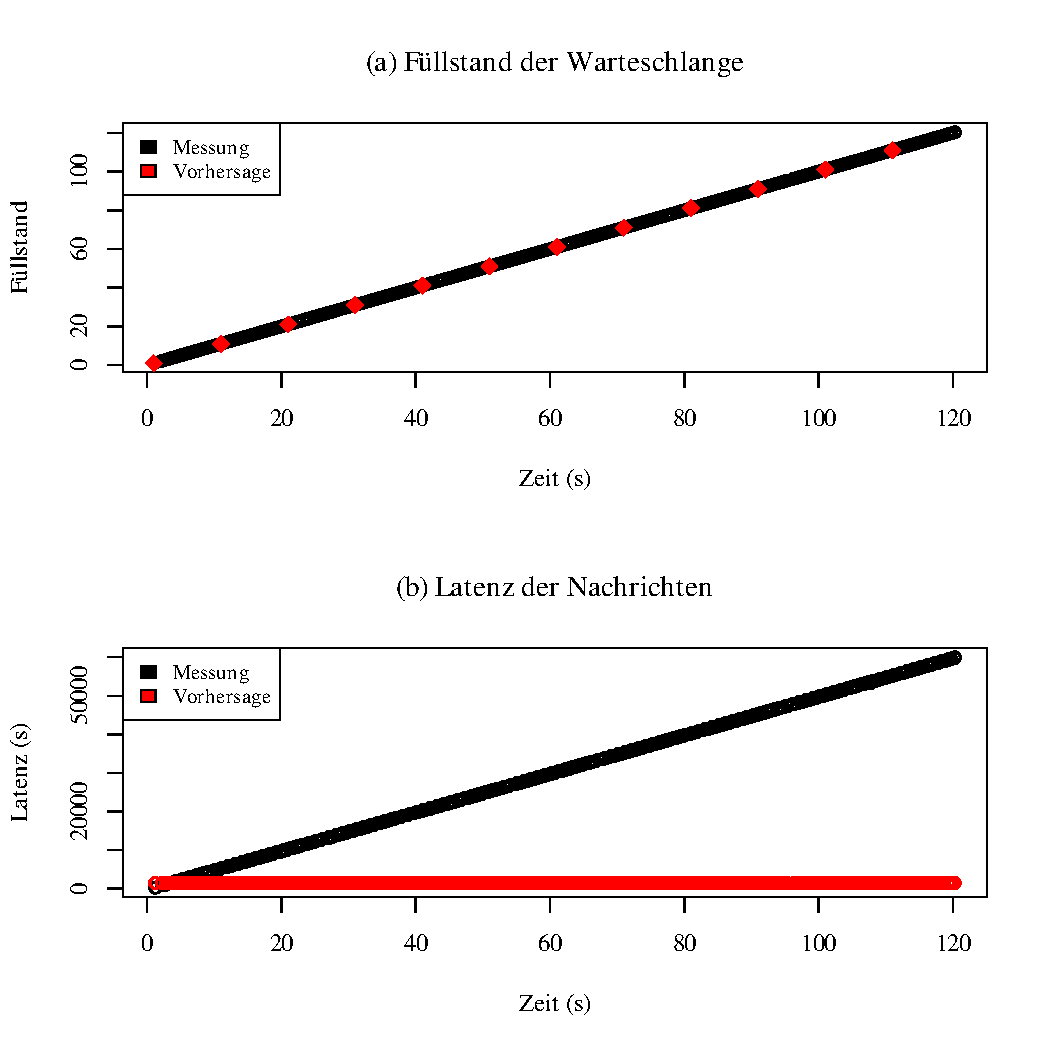
\includegraphics[width=0.5\textwidth]{images/modelSimulationResults/simulation3.pdf}
  \caption{Anwachsen der Warteschlange (Modell vs. Real System)}
  \label{img:simulation3}
\end{figure}

\subsubsection{Simulation 4}
Mit dieser Simulation soll die Auswirkung mehrerer Empfänger auf das System überpüft werden. Die Frage dabei ist, ob mehrere Empfänger eine Warteschlange gemeinsam abarbeiten können, wie in \autoref{sec:varyingConsumer} beschrieben. Obwohl in der Messung mit mehreren Empfängern, die Latenz nicht ganz an die Latenz eines Empfängers, der die Warteschlange alleine abarbeiten kann, herankommt, kann dieser Effekt aufgrund der minimalen Abweichung vernachlässigt werden. Im der folgenden Simulation ist die Ankunftszeit des Senders einmal pro Sekunde und die der beiden Empfänger jeweils einmal alle zwei Sekunden. Die Nachrichtengröße beträgt dabei, wie auch in der Messung, X Bytes. Betrachtet werden der Füllstand der Warteschlange und die Latenz der einzelnen Nachrichten. 
%B
\autoref{img:simulation4} zeigt die Ergebnisse der Simulation. In \autoref{img:simulation4}a ist der Zustand der Warteschlange abgebildet. Dabei ist zu sehen, dass die beiden Empfänger die Warteschlange gemeinsam abarbeiten können. Gleichzeitig ist in \autoref{img:simulation4}b zu sehen, dass sich die Latenz der Nachrichten normalisiert hat und konstant bleibt. Der Fehler liegt dabei bei X\%. 

\begin{figure}
\center
  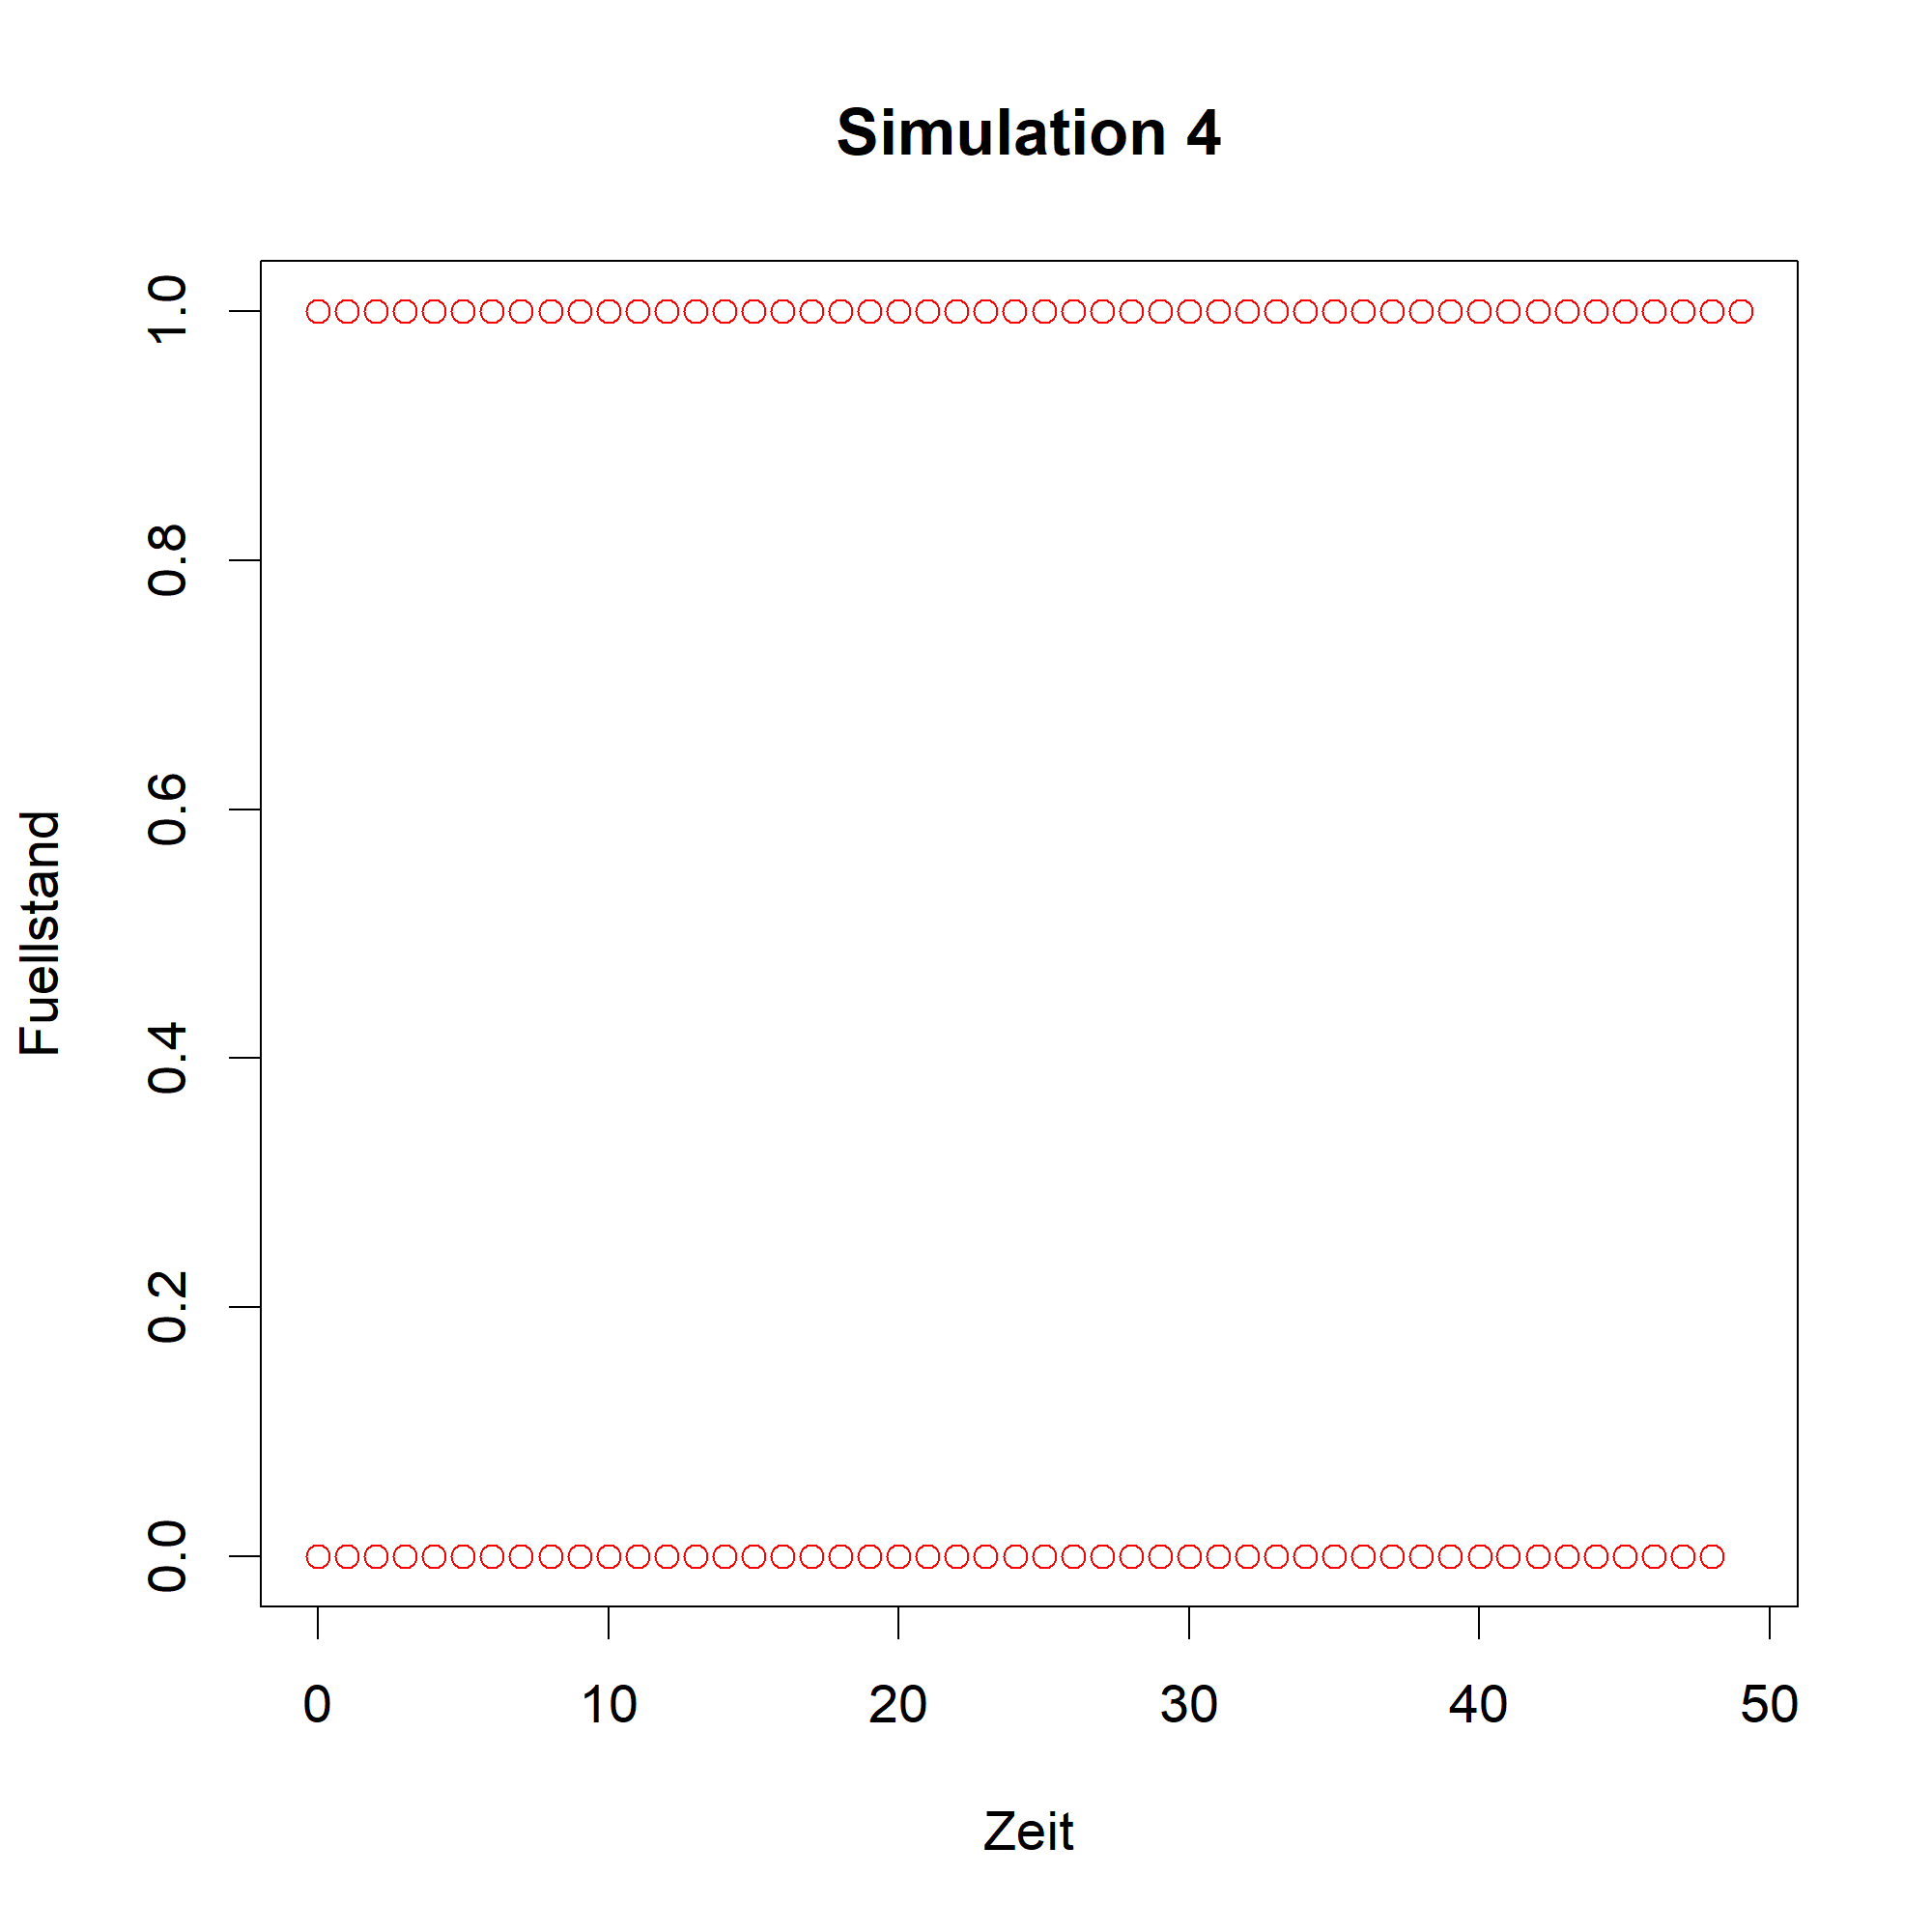
\includegraphics[width=0.5\textwidth]{images/modelSimulationResults/simulation4.png}
  \caption{Gemeinsames Abarbeiten einer Warteschlange durch zwei Empfaenger (Modell)}
  \label{img:simulation4}
\end{figure}

%Simulation 5: \\
%- Max Durchsatz \\
%- eine Nachricht mit max Bytesize schicken \\
%-> Response time sollte kontinuirlich ansteigen \\


\subsubsection{Simulation 5}
Schließlich betrachtet diese Simulation Lazy-Warteschlangen aus RMQ. Sender und Empfänger haben die gleiche Ankunftszeiten und kommen einmal pro Sekunde an. Die gesendete Nachrichten haben die Größe 100, 200, 300, 400, 500 und 1000 Kbyte. Der RD für eine Nachricht wurde im Modell angepasst. Dieser ist in \autoref{sec:rmqRd} beschrieben. Verglichen wurde mit der Messung aus \autoref{sec:rmqLazy}. Betrachtet wurde die Latenz der Nachrichten und der Füllstand der Warteschlange.
%B
Die Warteschlange bleibt aufgrunde der gleichen Ankuftszeiten gleich. In \autoref{img:simulation6} sind die Ergebnisse bezüglich der Latenz abgebildet. Neben den Vorhersagepunkten aus dieser Simulation und den Messpunkte aus der Messung mit Lazy-Warteschlangen, sind die Vorhersagepunkte aus \autoref{sec:rmqSimulation1} eingetragen. In (tabelle) sind die Fehler abgebildet. Dabei wird neben dem Fehler zur Messung mit Lazy-Warteschlangen und der Vorhersage mit Lazy-Warteschlangen auch der Fehler zwischen der Messung mit Lazy-Warteschlangen und der Vorhersage aus \autoref{sec:rmqSimulation1} berechnet. Dabei ist zunächst zu sehen, dass der Fehler zwischen der Messung und der Vorhersage mit Lazy-Warteschlangen zwischen X und Y liegt. Der Fehler zwischen der Messung mit Lazy-Warteschlangen und der Vorhersage aus \autoref{sec:rmqSimulation1} liegt zwischen A und B und ist somit höher. Somit ist zu sehen, dass die Anpassung des RD einen Einfluss auf die Genauigkeit der Vorhersage hat.
\begin{figure}
\center
  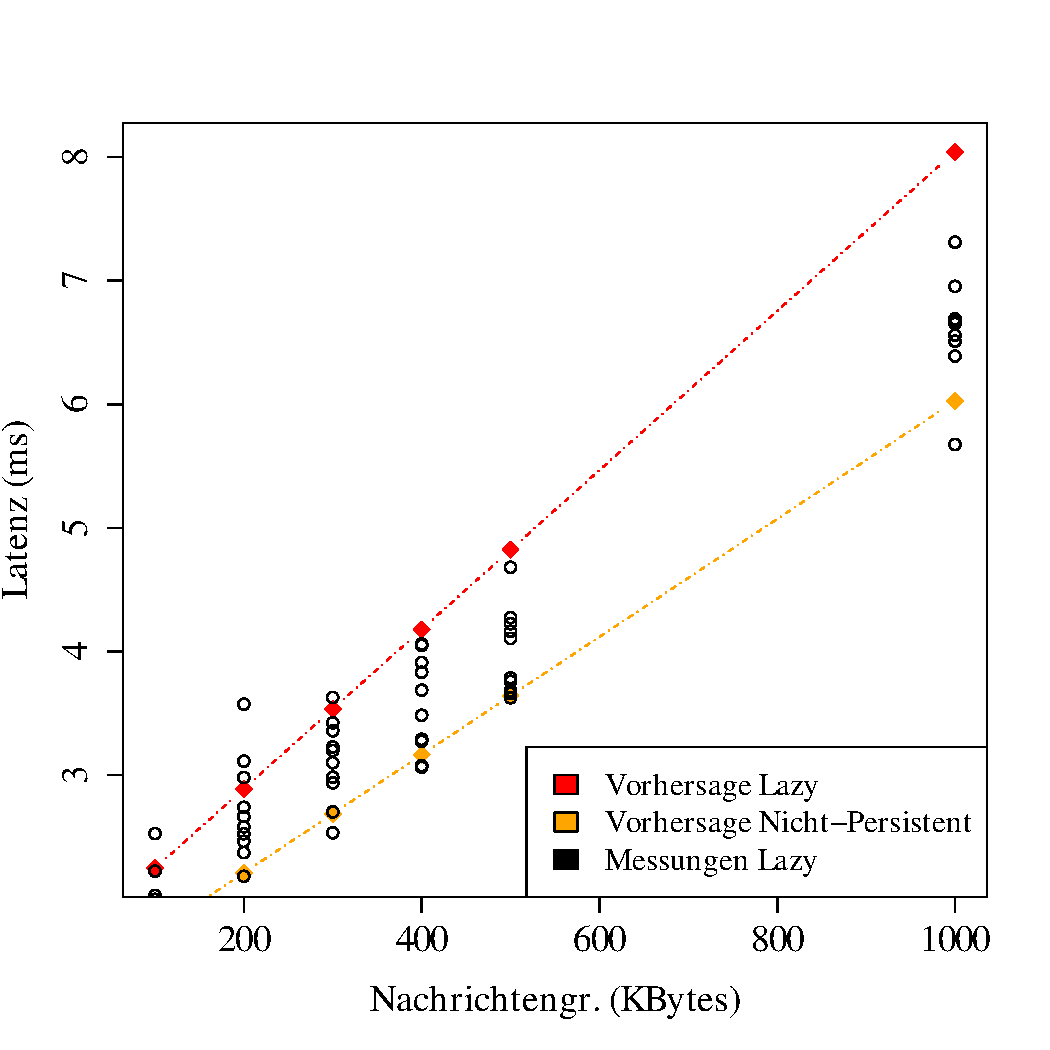
\includegraphics[width=0.5\textwidth]{images/modelSimulationResults/simulation6.pdf}
  \caption{Latenz einer Nachricht mit verschiedenen Groessen bei Lazy Warteschlangen (Modell vs. Real System)}
  \label{img:simulation6}
\end{figure}



\section{Grenzen}
Dieser Ansatz ermöglicht es jedoch nicht einzelne Nachrichten durch das System zu verfolgen\\

welche Moeglichkeiten gibt es? Dominiks Queue Modell. Direkt drauf verweisen, oder eine/diese Idee beschreiben.\\
%Queue Fuellstand ist unbekannt \\

%Nachdem eine MOM in das Experimentsystem eingebaut wurde, soll sie im Anschluss in Palladio modelliert werden. Wie bereits erwähnt existiert eine Palladio Modellierung des Experimentsystem, auf der aufgebaut werden kann. Bei der Modellierung der MOM soll zunächst die Standardkonfiguration und in späteren Iterationen Parametrisierbarkeit modelliert werden. Dazu soll zunächst versucht werden die MOM mithilfe vorhandener PCM Elementen zu modellieren und Unzugänglichkeiten zu identifizieren. Die Idee ist, mithilfe von Architecture-Templates \cite{architcturetemplate} diese Unzugänglichkeiten zu beseitigen. Dabei handelt es sich um wiederverwendbare Muster, die auf Palladio-Modelle angewendet werden können. Beispielsweise kann anstelle der manuellen Modellierung eines Lastverteilers auch das Architectural-Template für Lastverteiler verwendet werden. %Da diese Anwendung nur aus wenigen kleinen Schritten besteht, können Architekten viel Modellierungsaufwand einsparen.


%(-- RabitMQ Config:)\\% https://www.rabbitmq.com/configure.html\\
%(-- Kafka Config:)\\ %https://kafka.apache.org/documentation/#brokerconfigs 


%% LaTeX2e class for student theses
%% sections/evaluation.tex
%% 
%% Karlsruhe Institute of Technology
%% Institute for Program Structures and Data Organization
%% Chair for Software Design and Quality (SDQ)
%%
%% Dr.-Ing. Erik Burger
%% burger@kit.edu
%%
%% Version 1.3.3, 2018-04-17

\chapter{Transformation}
\label{ch:transformation}
Die zuvor vorgestellte Modellierung beschreibt, wie im PCM eine MOM mit expliziten Warteschlangen modelliert und kalibriert werden kann. Wie bereits diskutiert kann eine solche Modellierung sehr aufwändig sein. Ein Architekt muss für einer bestimmte Architektur die Auswirkung verschiedener MOMs untersuchen und vergleichen. Wie bereits beschrieben, stellt das PCM, seit der Arbeit von Rathfelder \cite{Rathfelder2013}, Modellelemente bereit, um event-basierte Komunikation abzubilden. Bevor eine Performance-Analyse durchgeführt wird, wird eine konkrete Middleware-Architektur in die Architektur eingewoben und die Event-Elemente ersetzt. Der Architekt muss somit nichts an seiner Gesamtarchitektur ändern und tauscht nur die Middleware-Architekturen aus. Ein solcher Ansatz soll auch in dieser Arbeit verwendet werden. Dazu sollen die Event-Elemente beibehalten werden und eine weitere Modelltransformation angeboten werden, um MOMs untersuchen zu können, die Warteschlangen explizit modellieren. Das Ziel ist es, dass ein Architekt zwischen mehreren MOMs auswählen kann, die zuvor kalibriert wurden, und diese in sein System einbauen kann. Im Folgenden wird beschrieben, wie eine solche Modelltransformation aussehen kann.
%Idee des Event Mechanismus: man moechte konkret ueber nachrichten/events reden und nicht abstrakt ueber interfaces. Event Transformation liefert am Ende Modell mit Interfaces usw. \\

\section{Transformationsprozess}
Zunächst soll beschrieben werden, wie ein solcher Transformationsprozess aussehen soll. Dieser ist in \autoref{img:transformationOverview} abgebildet. Der Softwarearchitekt beschreibt im ersten Schritt, wie zuvor auch, die Systemarchitektur und bildet event-basierte Kommunikation mithilfe der PCM-Event-Elemente ab. Es können auch bereits erstellte Event-Modelle verwendet werden. Im nächsten Schritt muss er sich für eine verfügbare MOM-Architektur entscheiden, deren Auswirkung auf das System er untersuchen möchte. Dazu kann er aus einer Sammlung von kalibrierten MOM-Bausteinen auswählen. Zum Zeitpunkt der Masterarbeit existiert nur ein RMQ-Baustein. Im nächsten Schritt kann er in einer Konfigurationsdatei bestimmte Konfigurationen festlegen. Im Anschluss wird die Systemarchitektur, die ausgewählte MOM und die Konfigurationsdatei mithilfe einer Modeltransformation transfomiert. Im Anschluss dienen die Ergebnissmodelle als Eingabe für die Performance-Analyse. Nach Durchführung der Performance-Analyse werden die Ergebnisse dem Architekten bereitgestellt.

\begin{figure}
\center
  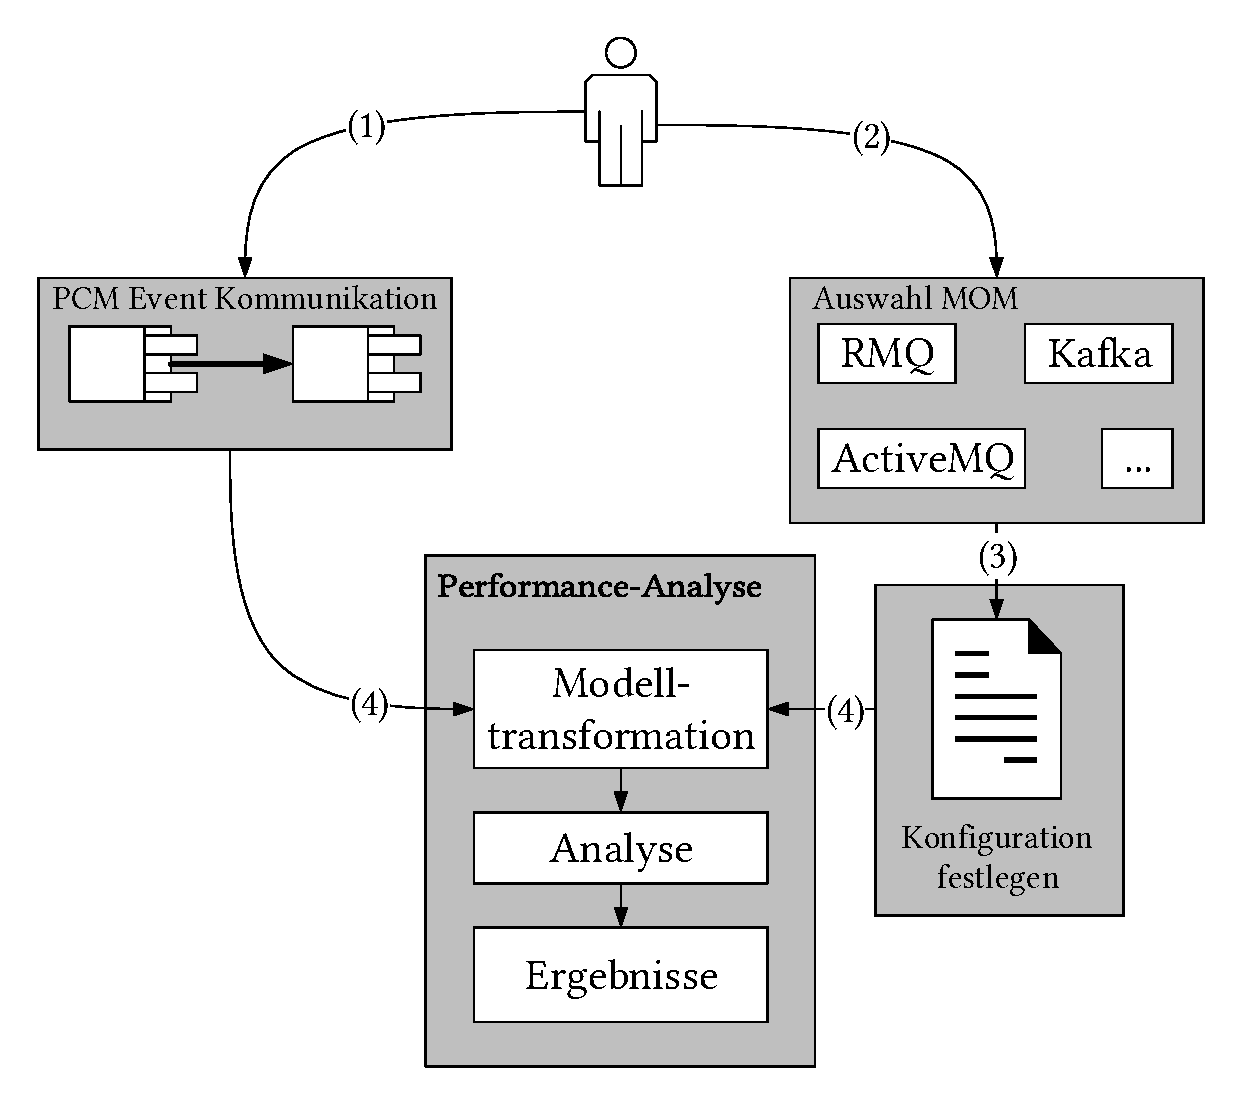
\includegraphics[width=1\textwidth]{images/transformation/transformationOverview.pdf}
  \caption{Übersicht des Transformationsprozess}
  \label{img:transformationOverview}
\end{figure}


\section{Konfiguration der MOM}
Wie bereits in den vorherigen Kapitel beschrieben, haben verschiedene MOMs auch diverse Möglichkeiten konfiguriert zu werden. Damit ein Architekt auch Konfigurationen einer MOM untersuchen kann, soll ihm die Möglichkeit geboten werden, bestimmte Konfigurationen einer MOM angeben zu können. Die möglichen Konfigurationen sind von der jeweiligen MOM abhängig. Für RMQ, die in dieser Masterarbeit untersuchte MOM, könnten folgende Konfigurationen angeboten werden:
\begin{itemize}
    \item Bereitstellen von Warteschlange: Welche Warteschlange wird auf welcher Ressource bereitgestellt. Dabei wird der Name des \emph{EventType}s angegeben, welchen die Warteschlange verarbeiten soll. Die Ressource auf der die Warteschlange bereitgestellt werden soll muss vor der Transformation bereits existieren. Außerdem kann Durchsatz und Latenz zu dieser Warteschlange angegeben werden.
    \item Lazy-Warteschlangen: Dabei kann angegeben werden ob die bereitgestellte Warteschlange eine Lazy-Warteschlange ist oder nicht. 
    \item Exchange-Zuständigkeit: Dabei kann festgelegt werden welche Warteschlange an welchen Exchange gebunden wird. Dabei kann ein Name für den Exchange und die Namen der dazugehörigen Warteschlangen angegeben werden. Der Name der Warteschlange ist dabei der \emph{EventType}, welchen die Warteschlange verarbeitet.
    \item Bereitstellen eines Exchange: Auf welcher Ressource wird der Exchange bereitgestellt. Außerdem kann Durchsatz und Latenz zu diesem Exchange angegeben werden.
\end{itemize}
In \autoref{img:configExample} ist eine Möglichkeit abgebildet, wie ein Architekt eine Konfiguration für einen RMQ-Baustein angeben kann. Dabei handelt es sich um eine XML-Datei. Zu sehen ist, dass es zwei Warteschlangen gibt. Die erste verarbeitet Nachrichten vom \emph{EventType} \texttt{Order}. Sie ist wird auf der Ressource \texttt{Middleware} bereitgestellt und ist eine Lazy-Warteschlange. Die zweite Warteschlange verarbeitet Nachrichten vom \emph{EventType} \texttt{OrderConf}. Auch sie wird auf der Ressource \texttt{Middleware} bereitgestellt. Sie ist jedoch keine Lazy-Warteschlange. Beide Warteschlange haben keinen Durchsatz und Latenz angegeben. Außerdem gibt es nur einen Exchange. Dieser wird ebenfalls auf der \texttt{Middleware} Ressource bereitgestellt. Er hat einen Durchsatz in Bytes und eine Latenz in Millisekunden angegeben. Die von ihm verwalteten Warteschlangen sind die beiden zuvor definierten Warteschlangen. Die hier vorgestellte Konfigurationsdatei ist nur ein Vorschlag, wie eine mögliche Konfiguration aussehen kann. Die Konfiguration kann auch in anderen Formen in die Transformation eingebunden werden, z.B. mithilfe von PCM-Profiles \cite{kramer2012b}.



\begin{figure}
\center
  \lstinputlisting[language=XML]{code/configExample.xml}
  \caption{Beispiel einer möglichen XML-Konfiguration für einen RMQ-Baustein.}
  \label{img:configExample}
\end{figure}

\section{Generierung von Exchange und Warteschlangen}
In \autoref{img:transformationRepository} ist die Transformation des Repository-Modells abgebildet. Im Ersten Schritt werden im Repository-Modell \emph{Exchange}-Komponenten eingefügt. Dabei wird die Anzahl und die Namen aus der Konfigurationsdatei ausgelesen. Außerdem werden die Ressourcen Anforderungen für Latenz und Durchsatz an die passende Stelle, der jeweiligen \texttt{Exchange}-Komponente, eingesetzt. Diese wurden in \autoref{sec:rmqRd} beschrieben. Die Komponenten werden wie im vorherigen Kapitel angeboten. Im nächsten Schritt wird jeder Sender identifiziert, der ein \emph{EventType} aussendet. Für diese Sender werden jeweils eine \emph{requiredRole} eingefügt, die eine der zuvor eingefügten \texttt{Exchange}-Komponente benötigt. Dabei werden die \emph{EventType}s beachtet. Jede \emph{EmitEventAction} eines Senders wird nun durch eine \emph{ExternalCallAction} ersetzt, die in der jeweiligen \texttt{Exchange}-Komponente die Funktion \texttt{Exchange.distribute} aufruft. Mithilfe einer \emph{UsageVariable} wird die Parameterbelegung festgelegt. Dabei wird als Typ der Name der zuvor aussendenden \emph{EventAction} angegeben. Außerdem wird eine Warteschlangen-Komponente angelegt die Nachrichten vom Typ \emph{EventType.name} entgegen nimmt. Bei der Erstellung werden außerdem passende Ressourcenanforderungen für eine Nachricht eingefügt. Diese werden aus der MOM-Konfiguration entnommen und an den passenden Stellen eingesetzt. Dies wurde in \autoref{sec:rmqRd} beschrieben. In der jeweiligen \texttt{Exchange}-Komponente, der für diesen \emph{EventType} zuständig ist, wird eine \emph{requiredRole} eingefügt, die diese Warteschlange benötigt. Als nächstes wird in den \texttt{distribute}-SEFF der \texttt{Exchange}-Komponente ein \emph{GuardedBranch} eingefügt. Die Bedingung lautet \texttt{Type == EventType.name}. Im Anschluss wird eine \emph{ExternalCallAction} eingefügt die die \texttt{Queue.put} Funktion in der zuvor erstellten Warteschlangen-Komponente aufruft. Nachdem alle Sender abgearbeitet wurden, wird nach allen Empfängern gesucht, die einen \emph{EventType} handhaben. Zunächst wird für diesen \emph{EventType} eine Schnittstelle mit dem Namen \texttt{IRecvX}, mit \texttt{X = EventType.name} angelegt. Diese Schnittstelle hat eine Signatur mit dem Namen \texttt{recvX}. Die Schnittstelle wird von dem aktuell betrachteten Empfänger angeboten. Außerdem wird eine \emph{requiredRole} erstellt, die die \texttt{Exchange}-Komponente benötigt, die dem \emph{EventType} zugeordnet ist. Ein SEFF wird erstellt, der die Funktionalität von \texttt{IRecvX.recvX} abbilden soll. Dieser enthält einen \emph{ExternalCallAction}, die die \texttt{Exchange.receive} in der benötigten \texttt{Exchange}-Komponente aufruft. Die Parameterbelegung wird mit einer \emph{UsageVariable}, mit \texttt{Type = EventType.name}, angegeben. Als nächstes wird im \texttt{receive}-SEFF der \texttt{Exchange}-Komponente eine \emph{BranchAction} eingefügt. Die Bedingung lautet \texttt{Type == EventType.name}. Im Anschluss wird eine \emph{ExternalCallAction} eingefügt die die \texttt{Queue.get} Funktion in der Warteschlangen Komponente aufruft, die Nachrichten vom Typ \emph{EventType} beinhalten.

\begin{figure}
\center
  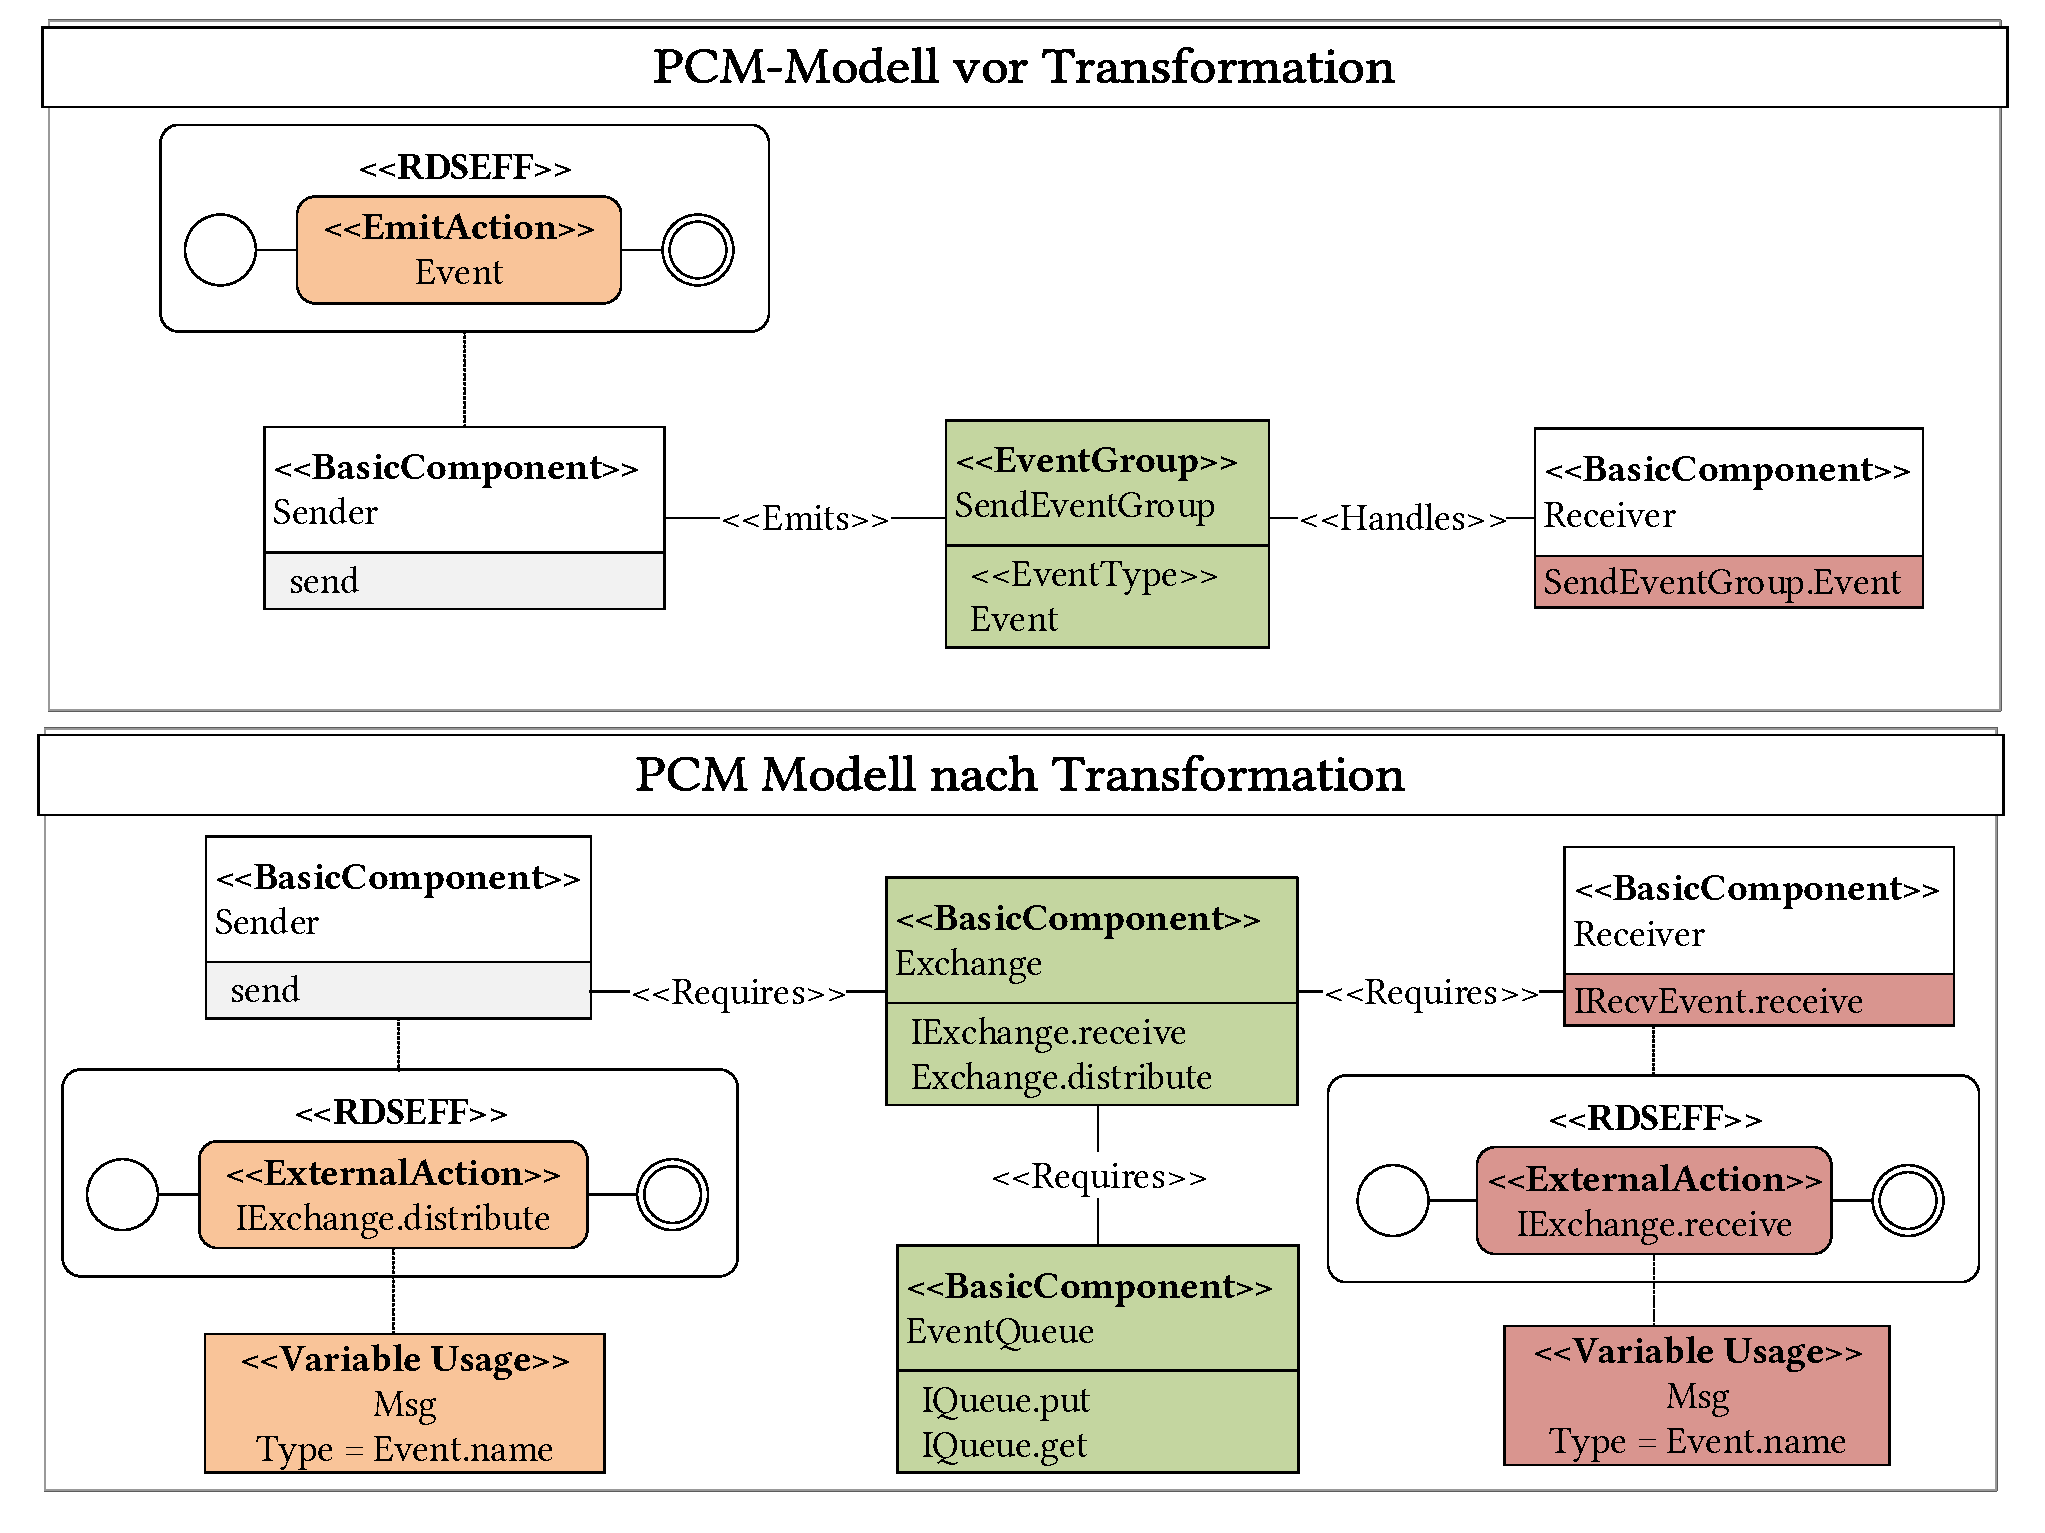
\includegraphics[width=1.3\textwidth, angle=90]{images/transformation/transformationRepository.pdf}
  \caption{Übersicht der Repository-Modell-Transformation}
  \label{img:transformationRepository}
\end{figure}


\section{Transformation von Punkt-Zu-Punkt Kommunikation}
Im Folgenden wird beschrieben, wie die Punkt-Zu-Punkt Kommunikation zwischen Komponenten transformiert wird. Eine Übersicht ist in \autoref{img:transformationP2P} abgebildet. Dabei wird das System- und Nutzungsmodell transformiert. Als erster Schritt werden die zuvor erstellen Exchange- und Warteschlangen-Komponenten im Systemmodell in einem \emph{AssemblyContext} eingefügt. Im Anschluss werden alle Warteschlangen mit der jeweiligen Exchange-Komponente über die passende Schnittstelle mit einem \emph{AssemblyConnector} verbunden. Als nächstes werden alle \emph{AssemblyEventConnector}s gesucht. Jeder \emph{AssemblyEventConnector} hat ein \emph{SourceRole} und ein \emph{SinkRole} Feld. Für jede \emph{SourceRole} wird die darin enthaltene Komponente über einen \emph{AssemblyConnector} mit der Exchange-Komponente verbunden. Die Komponente die sich im \emph{SinkRole}-Feld befindet wird ebenfalls mit der Exchange-Komponente, mithilfe eines \emph{AssemblyConnector}, verbunden. Außerdem wird für jedes der \emph{SinkRole}-Elemente eine \emph{SystemProvidedRole} erstellt. Die \emph{SinkRole}-Komponente und die \emph{SystemProvidedRole} werden mit einem \emph{DelegationsConnector} verbunden. Schließlich wird im Nutzungsmodell ein \emph{UsageScenario} angelegt um das Abholen von Nachrichten abzubilden. Dazu wird in dem \emph{UsageScenario} ein \emph{EntryLevelSystemCall} angelegt, der über die jeweilige \emph{SystemProvidedRole} Funktion \texttt{Exchange.receive} aufruft. Außerdem wird ein \emph{ClosedWorkload} mit \emph{Population} eins und einer \emph{ThinkTime} von null angelegt. Dadurch wird gewährleistet, dass eine Empfänger-Komponenten eine Nachricht aus der Warteschlange holt, sobald diese Verfügbar ist.

\begin{figure}
\center
  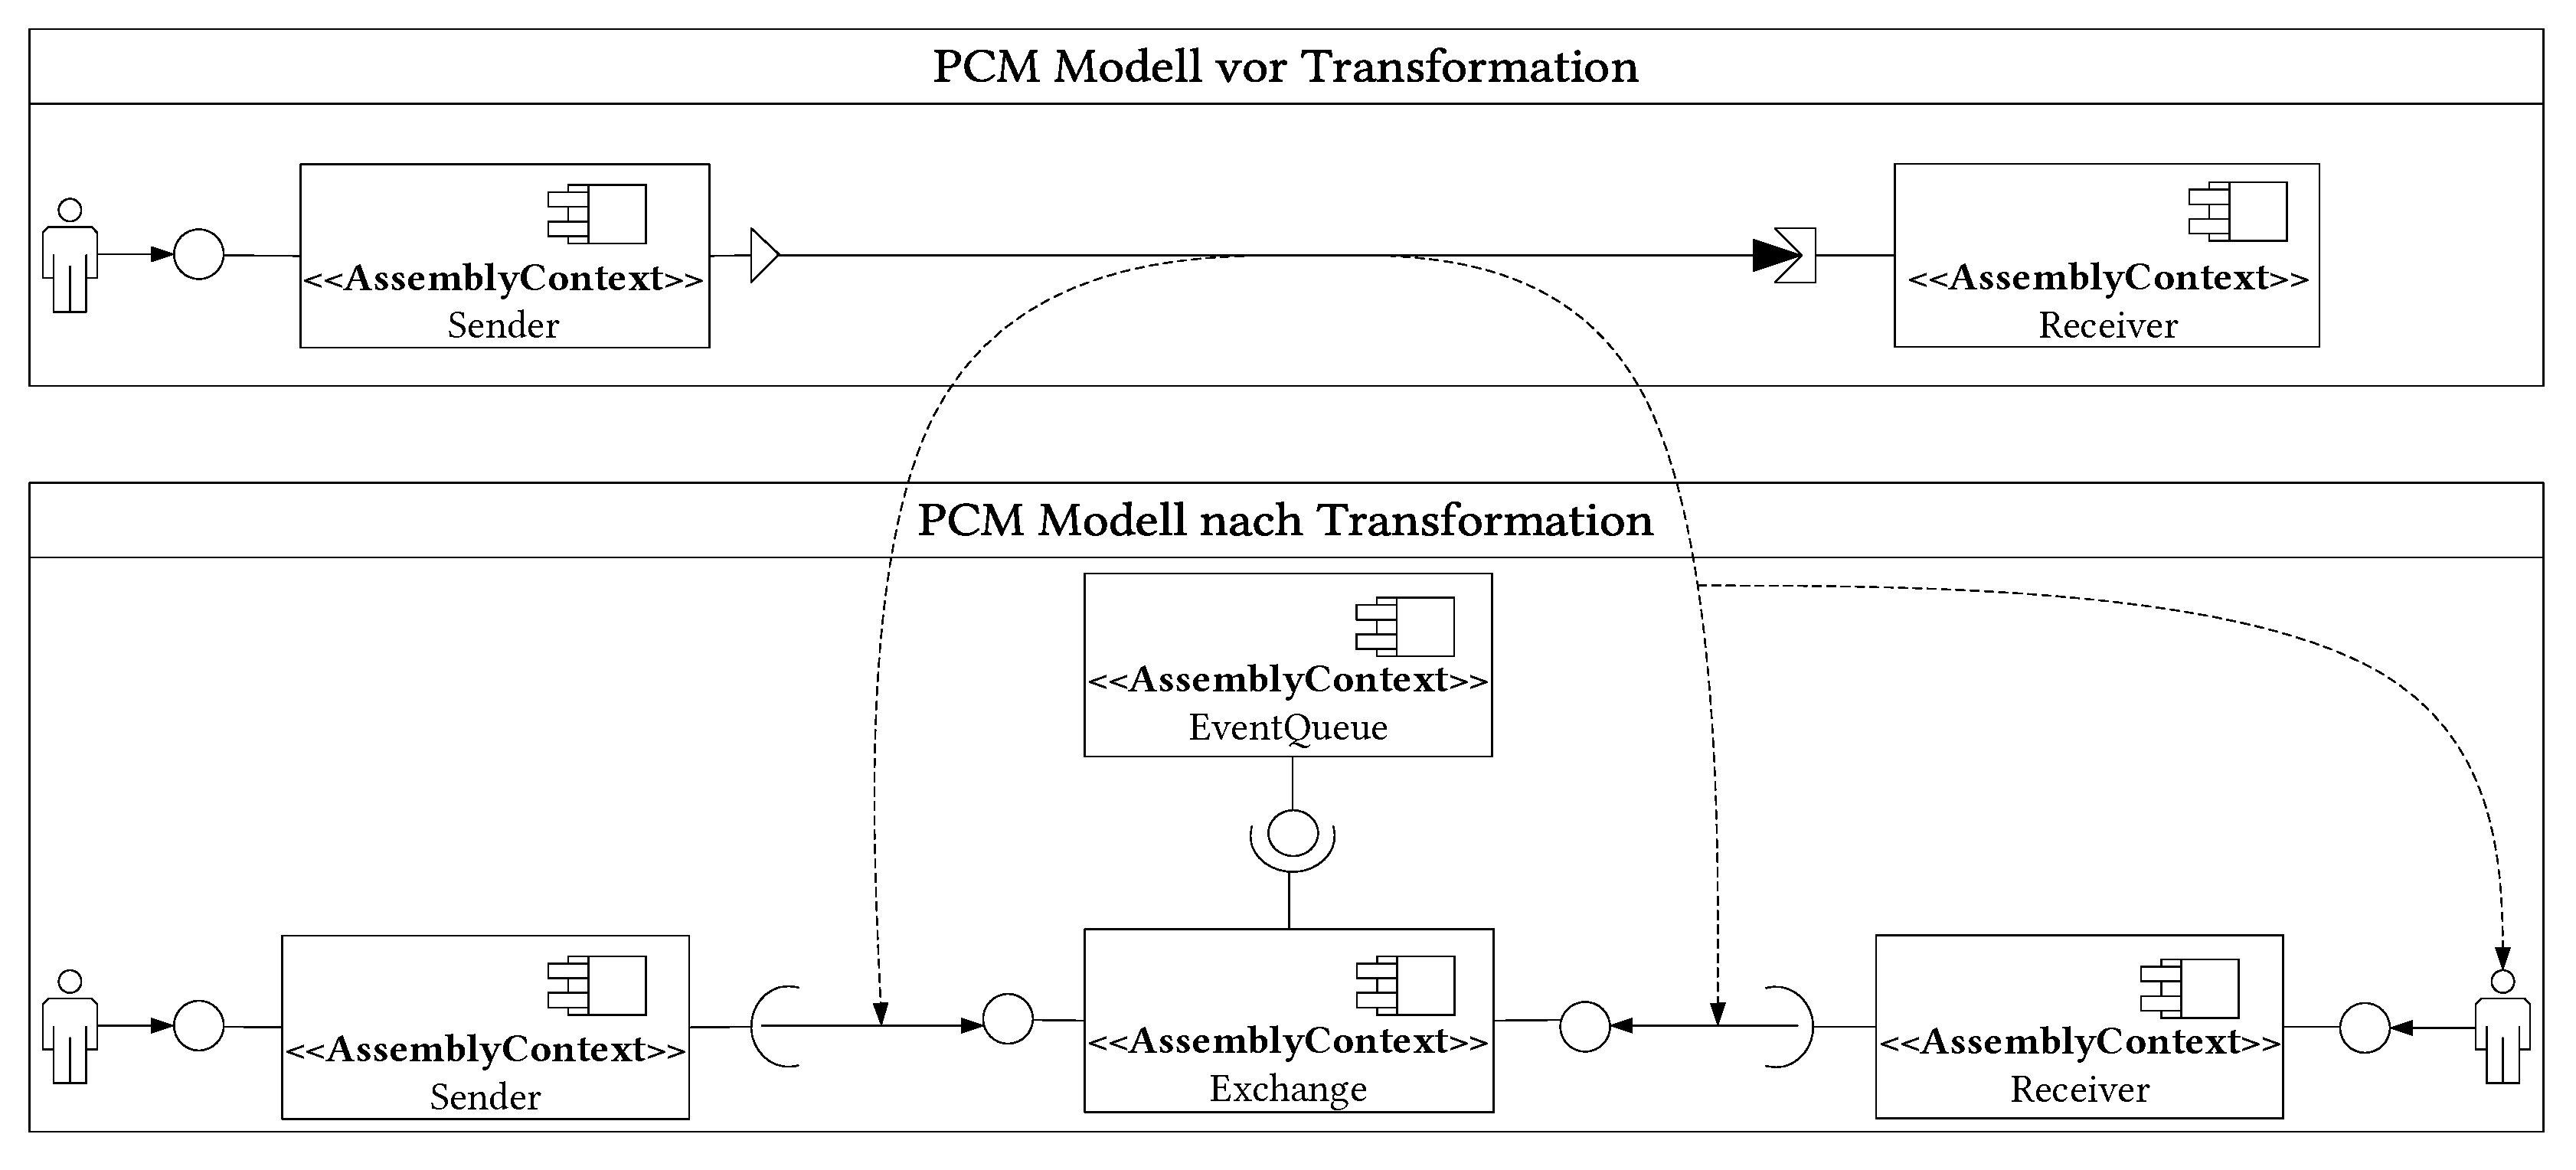
\includegraphics[width=1.3\textwidth, angle=90]{images/transformation/transformationSystemP2P.pdf}
  \caption{Übersicht der Punkt-Zu-Punkt-Transformation}
  \label{img:transformationP2P}
\end{figure}

\section{Transformation von Viele-Zu-Viele Kommunikation}
Im Fall von Viele-Zu-Viele Kommunikation werden neben dem System- und Nutzungsmodell auch das Repository-Modell angepasst. Eine Übersicht ist in \autoref{img:transformationPubSub} abgebildet. Die Viele-Zu-Viele Kommunikation findet in PCM über einen \emph{EventChannel} statt. Sender sind über eine \emph{SourceConnector} und Empfänger über einen \emph{SinkConnector} mit dem \emph{EventChannel} verbunden. Für jeden \emph{SourceConnector}, der die Sender-Komponente mit dem \emph{EventChannel} verbindet, wird ein \emph{AssemblyConnector} zwischen dem Sender und der jeweiligen Exchange-Komponente erstellt. Bei der Transformation der \emph{SinkConnector}en wird zunächst ein neuer \emph{AssemblyContext} mit Warteschlangen-Komponente erstellt. Im Repository-Modell wird in der Exchange-Komponente eine neue \emph{RequiredRole} angelegt die diese Warteschlange benötigt. Im \texttt{distribute}-SEFF wird der \emph{GuardedBranch} erweitert, der den dazugehörige \emph{EventType} behandelt. Für die zuvor erstellte \emph{RequiredRole} wird eine weiterer \emph{ExternalCallAction} erstellt, der die Nachricht an die Warteschlange sendet. Somit wird die Nachricht an mehrere Warteschlangen weitergeleitet. Im Systemmodell wird mit einem \emph{AssemblyConnector} die Exchange-Komponente und die Warteschlange verbunden. Außerdem wird für den Empfänger-\emph{AssemblyContext} eine \emph{SystemProvidedRole} erstellt und mit dem \emph{AssemblyContext}, mithilfe eines \emph{DelegationsConnector}s, verbunden. Schließlich wird, wie auch bei der Punkt-Zu-Punkt Transformation, im Nutzungsmodell eine \emph{UsageScanrio} angelegt. Damit soll das Abholen von Nachrichten abgebildet werden. In dem \emph{UsageScenario} wird ein \emph{EntryLevelSystemCall} angelegt, der über die jeweilige \emph{SystemProvidedRole} die \texttt{Exchange.receive} Funktion aufruft. Außerdem wird ein \emph{ClosedWorkload} mit \emph{Population} eins und einer \emph{ThinkTime} von null angelegt, damit eine Nachricht aus der Warteschlange geholt wird, sobald diese Verfügbar ist.

\begin{figure}
\center
  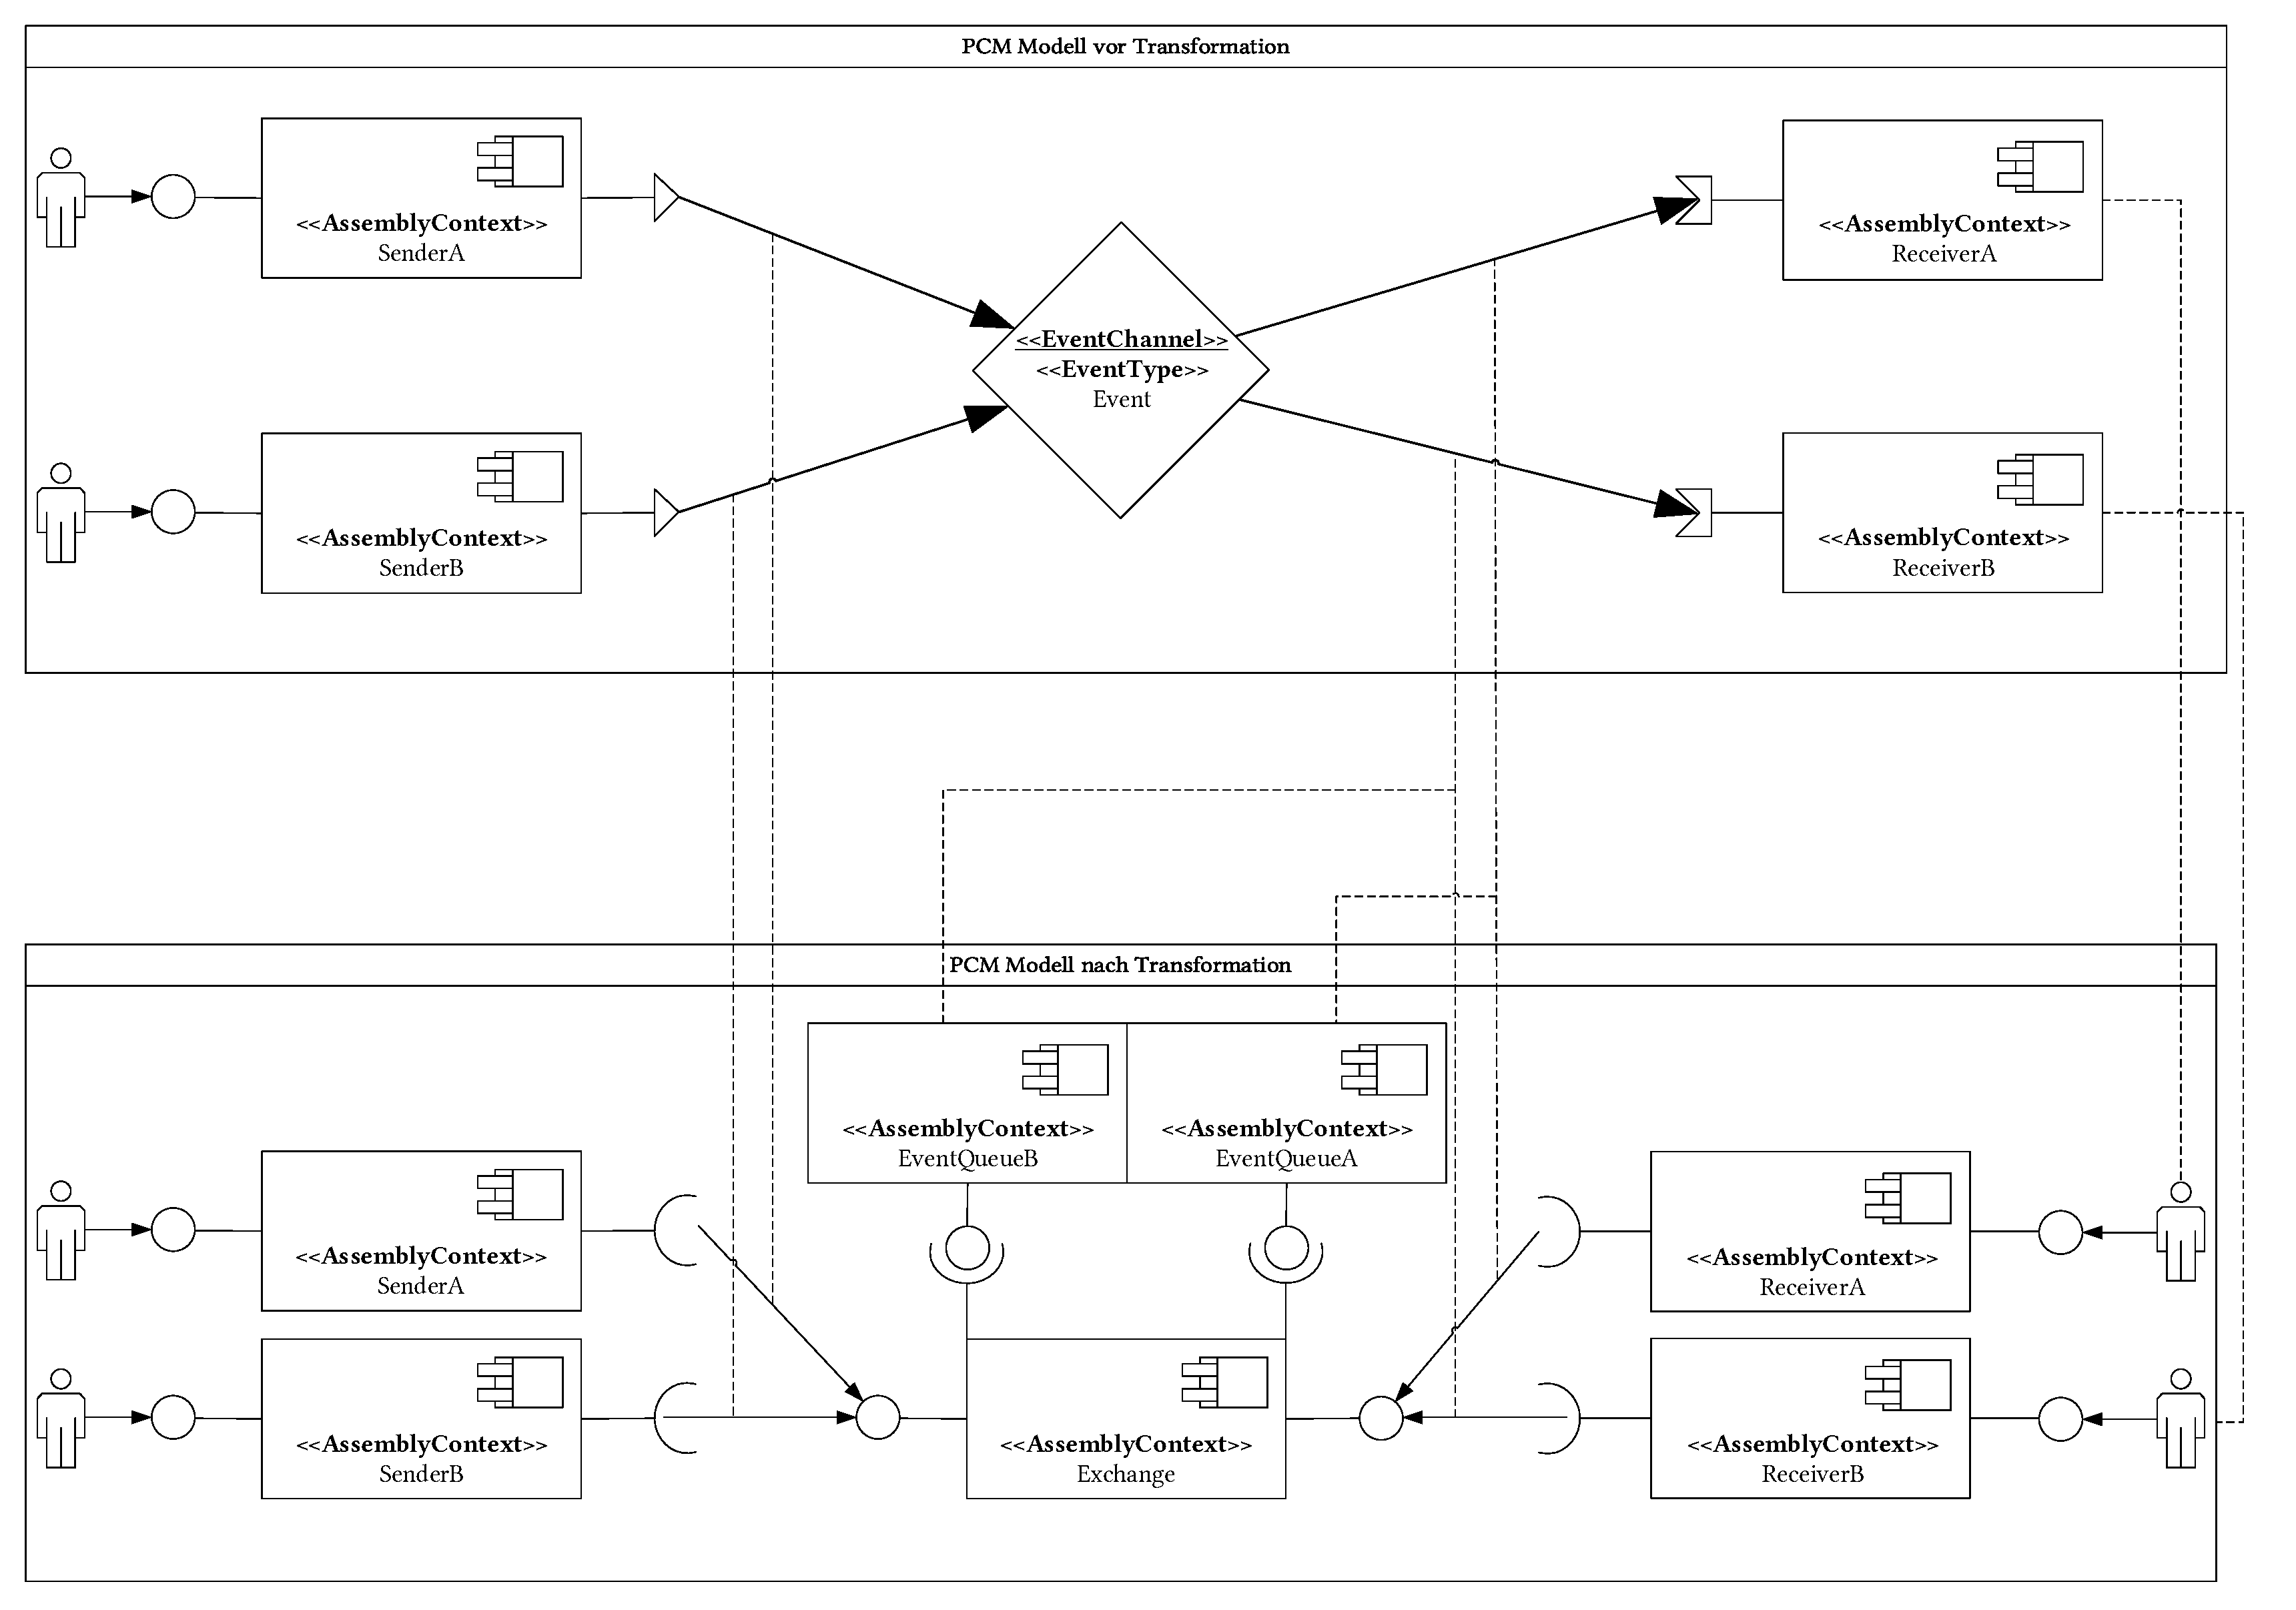
\includegraphics[width=1.4\textwidth, angle=90]{images/transformation/transformationSystemPubSub.pdf}
  \caption{Übersicht der Publish/Subscribe-Transformation}
  \label{img:transformationPubSub}
\end{figure}


\section{Bereitstellen der Komponenten}
Das Bereitstellen der Komponenten setzt voraus, dass in der vom Benutzer angegebenen Konfiguration festgelegt wurde, welche Warteschlangen- und Exchange-Komponente auf welcher Ressource bereitgestellt werden soll. Diese Ressourcen müssen bereits vor der Transformation erstellt worden sein. Währende der Transformation werden die Komponenten auf den Ressourcen im Allokations-Modell bereitgestellt. Dazu wird ein \emph{AllocationContext} erstellt auf der dazugehörigen Ressource bereitgestellt.


%% LaTeX2e class for student theses
%% sections/evaluation.tex
%% 
%% Karlsruhe Institute of Technology
%% Institute for Program Structures and Data Organization
%% Chair for Software Design and Quality (SDQ)
%%
%% Dr.-Ing. Erik Burger
%% burger@kit.edu
%%
%% Version 1.3.3, 2018-04-17

\chapter{Evaluation}
\label{ch:Evaluation}
Das Hauptziel dieser Masterarbeit ist es eine Modellierung einer MOM mit expliziten Warteschlangen zu ermöglichen und anschließend in Performance-Analysen zu untersuchen. Um dieses Ziel zu erreichen wurde in \autoref{ch:modellierung} eine Modellierungsmethode vorgestellt mit der eine MOM modelliert und kalibriert werden kann. Die in \autoref{ch:mom} ausgemessenen Ergebnisse wurden dabei zum Kalibrieren der Modelle verwendet. Im Folgenden, soll die bisherige Arbeit evaluiert werden und dabei gezeigt werden, dass die definierten Ziele erreicht werden konnten. 

Die Ziele und die Bewertung, ob diese erreicht werden konnten werden mithilfe der Goal-Question-Metric (GQM) untersucht.
Die GQM-Methode \cite{gqm} spezifiziert Ziele für das zu evaluierende Konzept. Daraufhin werden zu den Zielen Fragen spezifiziert, mit denen die Erfüllung des Ziels überprüft werden soll. Schließlich werden Metriken festgelegt, durch die die Fragen beantwortet werden sollen. Aus \autoref{tab:gqm} können die Ziele, Fragen und Metriken entnommen werden, mit denen diese Masterarbeit evaluiert werden soll.

Ein Ziel, das mithilfe dieser Masterarbeit erreicht werden soll, ist die Modellierung von MOMs in Palladio zu ermöglichen. Das zweite Ziel ist es, Vorhersagen mithilfe der Performance-Analyse zu ermöglichen und dadurch die Entscheidungsfindung, welche MOM verwendet werden soll, bereits zur Modellierungszeit und aus Architekturperspektive zu verbessern. Die dazu definierten Fragen prüfen ob mithilfe der Modellierung sowohl Punkt-Zu-Punkt, als auch Publish/Subscribe-Kommunikation vorhergesagt werden können. Dabei dient der Fehler zwischen Messung und Vorhersage als Metrik. In der Literatur ist ein Fehler zwschen 35\% und 40\% akzeptiert \cite{error}.

Im Folgenden wird in \autoref{sec:specjms} der SPECjms2007 Benchmark vorgestellt, mit dem die Evaluierung durchgeführt wird. Anschließend werden in \autoref{sec:specjmsmodell} die PCM-Modellierung des Benchmarks beschrieben. Im Anschluss wird in \autoref{sec:specjmsmodellvorhersage} die Vorhersagegenauigkeit der Modellierung untersucht. Schließlich werden in \autoref{sec:evaluationzusammenfassung} die Ergebnisse zusammengefasst und diskutiert. 
\begin{table}
  \begin{tabular}{|l|l|}
    \hline
    \multicolumn{2}{|l|}{Ziel 1} \\
    \hline
    Zweck & Ermögliche \\
    Qualitätskriterium & eine wartbare und wiederverwendbare Möglichkeit  \\ 
    Prozess & eine MOM zu modellieren \\
    Sicht & aus Architekturperspektive \\
   
    \hline \hline
    \multicolumn{2}{|l|}{Ziel 2} \\
    \hline
    Zweck & Verbessere \\
    Qualitätskriterium & die Abwägung und Entscheidungsfindung  \\ 
    Prozess & beim Einsatz einer MOM \\
    Sicht & aus Architekturperspektive \\
    \hline \hline
    Frage 1 & Lässt sich die Latenz einer Nachricht für Punkt-Zu-Punkt \\
    & Kommunikation vorhersagen? \\
    \hline
    Metrik & Fehler in \% zwischen Messung und Vorhersage? \\
    \hline \hline
    Frage 2 & Lässt sich die Latenz einer Nachricht für Publish/Subscribe-\\
    & Kommunikation vorhersagen? \\
    \hline
    Metrik & Fehler in \% zwischen Messung und Vorhersage? \\
    \hline
  \end{tabular}
	\caption{\label{tab:gqm} Ziele, Fragen und Metriken für die Evaluierung, nach der GQM-Methode}
\end{table}


%\section{Systemanforderungen}
%\label{sec:systemanforderungen}
%Für das Evaluierungssystem wurden im Folgenden Anforderungen festgelegt.
%\begin{itemize}
%\item Das jeweilige System soll \textbf{Skalierung} erlauben. Dabei soll es zum einen möglich sein die Anzahl von Kommunikationspartnern zu erhöhen (\textit{horizontal}) als auch die Menge an Nachrichten die verschickt werden (\textit{vertikal}).
%\item Weitere \textbf{Konfigurationen} wie Nachrichtengröße, reihenfolgentreue, Duplikate, etc. sollten möglich sein.
%\item System soll möglichst \textbf{reales System} darstellen.
%\item Mindestens ein \textbf{Nachrichtenmodell} sollte unterstützt werden.
%\item Es sollten \textbf{verschiedene Interaktionstypen} unterstützt werden, wie Many-To-Many, Many-To-One, etc.
%\item Damit der Fokus der Masterarbeit auf den MOMs und ihrer Modellierung liegt, sollte das System \textbf{bereits vorhanden} und implementiert und modelliert sein.
%\end{itemize}

\section{SPECJms2007}
\label{sec:specjms}
Das für die Evaluierung verwendete System ist das im SPECJms2007 Benchmark verwendete Testsystem \cite{Sachs2013}. Der Benchmark stellt eine reale ereignisbasierte Anwendung dar und umfasst eine Reihe von verschiedener Interaktionen, die sowohl Punkt-zu-Punkt- als auch Publish/Subscribe-Nachrichten einschließlich One-to-One-, One-to-Many- und Many-to-Many-Kommunikation umfasst. Das Hauptziel des SPECjms2007 Benchmarks ist es, einen Standard-Workload bereitzustellen, der die Leistung und Skalierbarkeit von JMS-basierten Message-Oriented Middleware-Plattformen bewertet. Bei dem System handelt es sich um ein Lieferkettenmanagement für eine Supermarktkette. Der Benchmark verwendet verschiedene Nachrichtentypen und verwendet Nachrichten verschiedenen Größe. Für die Masterarbeit liegt sowohl die Implementierung des Benchmarks, als auch eine Modellierung aus einer früheren Arbeit von Christoph Rathfelder \cite{Rathfelder2013} vor. Dieses System soll als Experimentsystem verwendet werden um die verschiedenen MOMs zu vergleichen und zum kalibrieren der später erstellten Modellierung. 

\subsection{Anwendungsszenario}
Das gewählte Anwendungsszenario bildet die Lieferkette eines Supermarktunternehmens ab. In \autoref{img:specjmsInteraction} sind die beteiligten Rollen abgebildet und wie sie miteinander kommunizieren. Die beteiligten lassen sich wie folgt gruppieren: 
\begin{itemize}
    \item Hauptquartier (HQ): Für die Buchhaltung des Unternehmens verantwortlich. Beobachtet den Geld und Warenfluss im System. Verwaltet Informationen ueber Waren und definiert Preise.
    \item Supermarkt (SM): Verkauft Waren an Kunden. Im Benchmark liegt der Fokus auf der Verwaltung der eigenen Warenlager. Jeder SM ist mit einem Vertriebszentrum verbunden.
    \item Vertriebszentrum (DC): Beliefert SM mit Waren. Ein DC nimmt Aufträge von SMs an und liefert diese. Wenn ein DC die Waren nicht vorrätig hat, werden diese Waren von einem Zulieferer angefordert. Außerdem sind DCs dafür verantwortlich Verkaufsstatistiken an das HQ zu senden.
    \item Zulieferer (SP): SPs sind nicht Teil des Supermarktunternehmens. Jeder SP bietet eine bestimmte Art von Waren an. Diese werden an DCs geliefert, wenn angefordert.
\end{itemize}

\begin{figure}
\center
  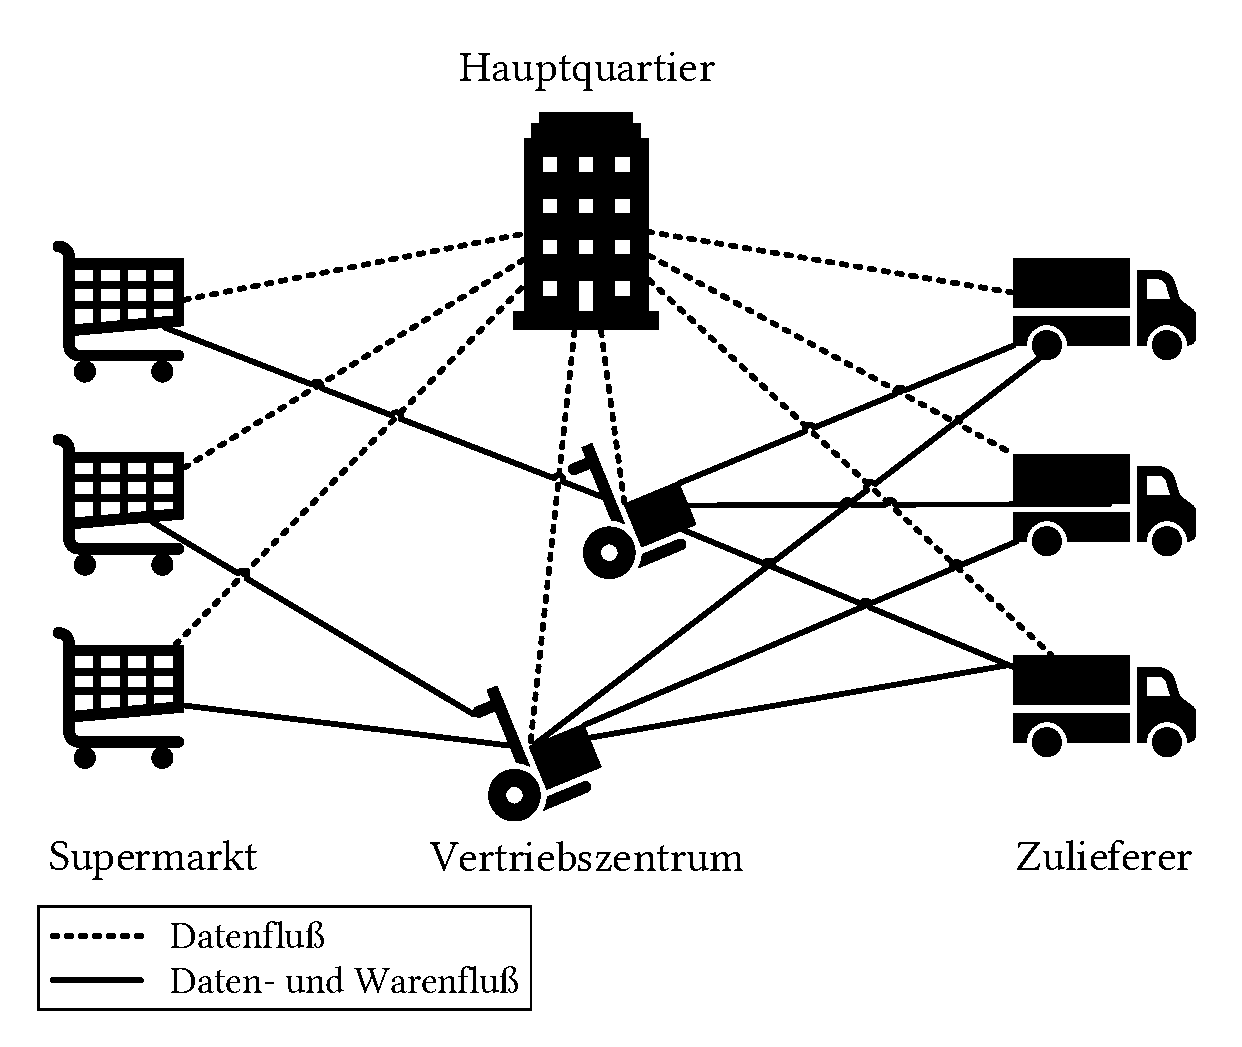
\includegraphics[width=0.7\textwidth]{images/evaluation/specjms/specjmsOverview.pdf}
  \caption{Anwendungszenario des SPECjms2007 Benchmark}
  \label{img:specjmsInteraction}
\end{figure}

\subsection{Interaktionen und Kommunikation}
SPECjms2007 sieht insgesamt sieben verschiedenen Interaktionsmöglichkeiten vor: 
\begin{enumerate}
    \item Bestell- und Versandabwicklung zwischen SM und seinem DC (Punkt-Zu-Punkt).
    \item Bestell- und Versandabwicklung zwischen DC und seinen SPs (Punkt-Zu-Punkt und Publisher/Subsciber).
    \item Preisaktualisierung (Publisher/Subsciber).
    \item Inventurmanagmenet (Punkt-Zu-Punkt).
    \item Verkaufsstatistik Sammlung (Punkt-Zu-Punkt).
    \item Bekanntmachungen zu Produkten (Publisher/Subsciber).
    \item Kreditkarten Hot-List (Publisher/Subsciber).
    
\end{enumerate}
Im Rahmen der Masterarbeit wurden (, aus Zeitlichen Gründen,) zwei dieser Interaktionen betrachtet. Um trotzdem verschiedene Nachrichtenmodelle und Interaktionstypen betrachten zu können wurden die folgenden beiden Interaktionen ausgewählt.
%warum wurden nur 2 und wiese genau diese ausgewaehlt? (Zeit, welche kommunikationsarten konnten abgedeckt werden?)\\
%Nachrichtenmodelle mit einbeziehen \\
%Interaktionstypen mit einbeziehen \\
\subsubsection{Interaktion 1}
\label{sec:interaction1desc}
Diese Interaktion übt Punkt-Zu-Punkt Kommunikation zwischen einem SM und seinem DC und dem DC und dem HQ aus. Dabei werden persistenten Nachrichten gesendet. Die Interaktion wird ausgelöst, wenn Waren im Lager eines SM aufgebraucht sind. Der SM bestellt bei einem DC Nachschub um seine Waren aufzufüllen. Neben dem SM und DC ist das HQ auch an dieser Interaktion beteiligt. In \autoref{img:specjmsInteraction1seq} ist der Ablauf als Sequenzdiagramm abgebildet. 
\begin{itemize}
    \item Der SM sendet eine Bestellung an seinen DC (\emph{Order}).
    \item Der DC sendet eine Bestätigung, über den Eingang der Nachricht zurück an den SM (\emph{OrderConf}).
    \item Die bestellte Ware wird registriert während sie das Warenlager des DC verlässt (\emph{ShipDep}).
    \item Der DC sendet Informationen über die Transaktion an HQ (\emph{StatInfoOrder}).
    \item Die bestellte Ware wurde vom DC an SM gesendet und empfangen (\emph{ShipInfo}).
    \item Der SM sendet eine Bestätigung über den Erhalt der Bestellung an DC (\emph{ShipConf})
\end{itemize}
%Zunächst sendet der SM eine Order Nachricht an den DC. Der DC bestätigt dem SM den Eingang der Nachricht. Als nächstes werden die Waren verschickt. Dabei werden sie von einem RFID Leser erfasst. Schließlich sendet der DC Informationen über die Transaktion an das HQ. Sobald die Lieferung beim SM ankommt wird eine Bestätigung an DC gesendet.

\begin{figure}
\center
  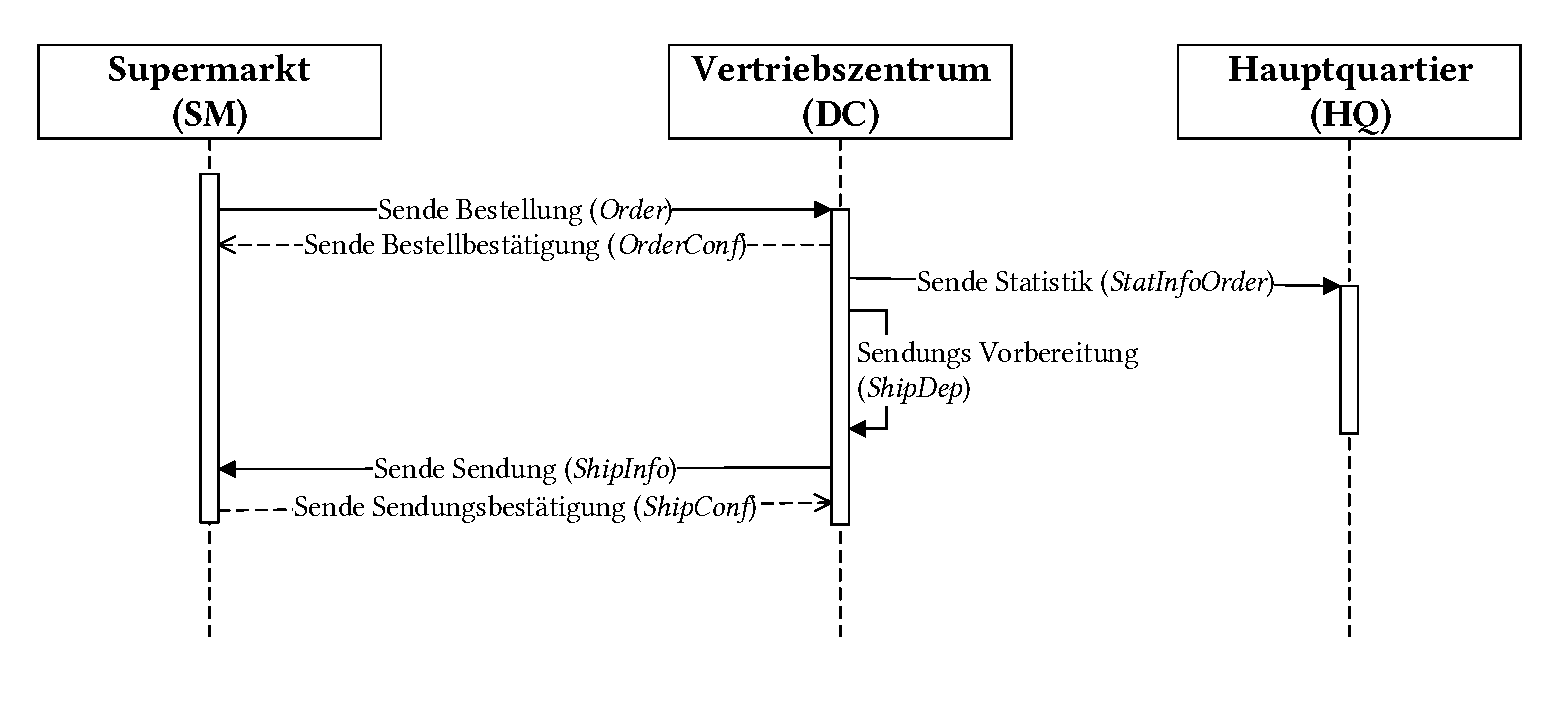
\includegraphics[width=1\textwidth]{images/evaluation/specjms/evaluationInteraktion1seq.pdf}
  \caption{Sequenzdiagramm von Interaktion 1 des SPECjms2007}
  \label{img:specjmsInteraction1seq}
\end{figure}

\subsubsection{Interaktion 3}
\label{sec:interaction3desc}
Diese Interaktion übt Publisher/Subscriber Kommunikation zwischen dem HQ und seinen SMs aus. Dabei werden persistenten Nachrichten versendet. Es handelt sich um eine Eins-Zu-Viele Kommunikation und wird ausgelöst, wenn die Preise der Ware durch die Firmenleitung (HQ) geändert werden. Um dies zu kommunizieren, sendet das HQ Nachrichten an alle SMs. In \autoref{img:specjmsInteraction3seq} ist der Ablauf der Interaktion als Sequenzdiagramm abgebildet. In der Standardkonfiguration komuniziert ein HQ mit zehn SMs.
\begin{itemize}
    \item Das HQ sendet ein Preisaktualisierung (\emph{PriceUpdate}).
    \item Betroffene SMs empfangen und ändern die Information in ihrem System.
\end{itemize}


\begin{figure}
\center
  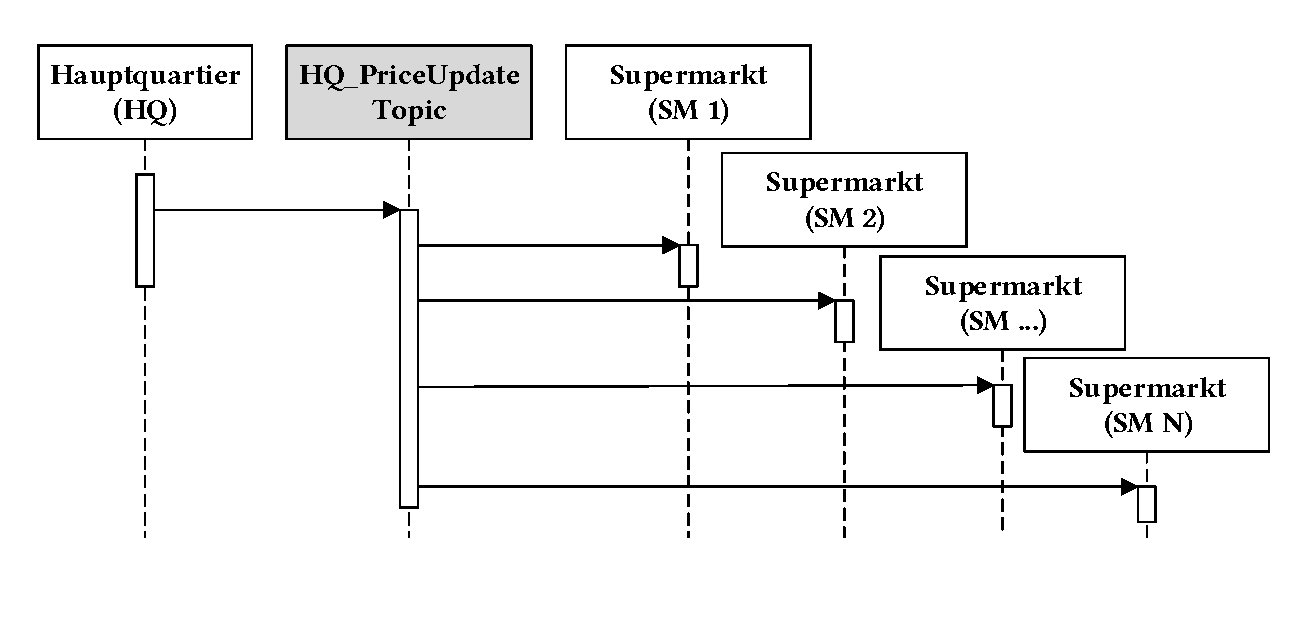
\includegraphics[width=1\textwidth]{images/evaluation/specjms/evaluationInteraktion3seq.pdf}
  \caption{Sequenzdiagramm von Interaktion 3 des SPECjms2007}
  \label{img:specjmsInteraction3seq}
\end{figure}


\subsection{Konfiguration}
SpecJMS2007 erlaubt verschiedene Konfigurationen durch den Benutzer. Dabei kann die Topologie sowohl horizontal, als auch vertikal skaliert werden. Bei der horizontalen Skalierung, wird die Anzahl der Akteure erhöht, während die Anzahl der gesendeten Nachrichten pro Akteur gleich bleibt. Die vertikale Topologie erhöht die Anzahl der Nachrichten die die Sender senden. Beide Skalierungsarten werden in einer eigenen Konfigurationsdatei mithilfe des Parameters BASE eingestellt.

Außerdem lassen sich für jede Nachricht die Größe und die Verteilung festlegen, mit welcher Wahrscheinlichkeit eine bestimmte Nachrichtengröße auftritt. Die Nachrichtengröße wird dabei mit folgender Formel berechnet: 
\[m1 + x * b\] 
Dabei kann x vom Benutzer des Benchmarks eingestellt werden. Die beiden anderen Parameter wurden in der Arbeit von Sachs et al.\cite{Sachs2013} hergeleitet. Somit kann für jede Nachricht die Wahrscheinlichkeit und ihre Größe festgelegt werden. In \autoref{tab:parameters} sind die für diese Arbeit wichtigen Parameter abgebildet. Die Verteilungen und die dazugehörige Nachrichtengrößen sind in \autoref{tab:msgpropandsize} abgebildet.


\begin{table}
\center
  \begin{tabular}{|c|l|l|l|}
  \hline
    \textbf{Interaktion} & \textbf{Nachricht} & \textit{m1} & \textit{b}  \\
    \hline \hline
    \multirow{6}{*}{1} & Order & 0,0565 & 1,4534 \\\cline{2-4}
    & OrderConf & 0,0565 & 1,4534 \\\cline{2-4}
    & ShipDep & 0,0787 & 0,7222 \\\cline{2-4}
    & StatInfoOrder & 0,0153 & 0,1463 \\\cline{2-4}
    & ShipInfo & 0,0787 & 0,8912 \\\cline{2-4}
    & ShipConf & 0,0202 & 0,7140  \\\hline
    \hline
     3 & PriceUpdate & - & 2,310 \\\hline
  \end{tabular}
	\caption{\label{tab:parameters} Parameter zur Berechnung der Nachrichtengröße. Auszug aus Sachs et al.\cite{Sachs2013}}
\end{table}

\begin{table}
\center
  \begin{tabular}{|c|l|l|l|l|}
  \hline
    \textbf{Interaktion} & \textbf{Nachricht} & \textbf{Größe 1} & \textbf{Größe 2} &\textbf{Größe 3} \\
     & \textit{Wahrscheinlichkeit} & \textit{95\%}  & \textit{4\%} &\textit{1\%}   \\
    \hline \hline
    \multirow{6}{*}{1} & Order & 1,74 & 7,10 & 41,01 \\\cline{2-5}
    & OrderConf & 2,02 & 7,39 & 41,29 \\\cline{2-5}
    & ShipDep & 1,12 & 8,59 & 55,79\\\cline{2-5}
    & StatInfoOrder & 0,22 & 1,67 & 10,83 \\\cline{2-5}
    & ShipInfo & 1,28 & 8,76 & 55,95 \\\cline{2-5}
    & ShipConf & 0,81 & 2,73 & 14,83  \\\hline
    \hline
     3 & PriceUpdate & 0,24 & 0,24 & 0,24 \\\hline
  \end{tabular}
	\caption{\label{tab:msgpropandsize} Nachrichtengröße in KByte. Auszug aus Sachs et al.\cite{Sachs2013}}
\end{table}

\section{Beschreibung der PCM-Modelle}
\label{sec:specjmsmodell}
In der Arbeit von Rathfelder \cite{Rathfelder2013} wurde SpecJMS auch als eines von zwei Fallbeispielen verwendet. Dabei ist eine PCM-Modellierung des Systems entstanden. Teile der Modellierung wurden für die Evaluierung dieser Masterarbeit wiederverwendet. Dabei handelt es sich um die Teile, die die Interaktion ein und drei beschreiben. Im Folgenden werden diese PCM-Modell-Teile beschrieben. Außerdem werden Änderungen an den Modellen, sowie ihr Aussehen nach der in \autoref{ch:transformation} beschriebenen Transformation, besprochen. 

\subsection{Repository und Systemmodell}
Die Akteure, SM, DC, SP und HQ, des Benchmarks sind in der Modellierung jeweils als eine Komponente modelliert. Die einzelnen Nachrichten die durch das System versendet werden, sind jeweils als eigener EventType modelliert. Diese EventTypes werden zur Kommunikation zwischen den Komponenten verwendet. Für jede Komponenten wurde eine SourceRole und SinkRole angegebn, die sich auf den EventType bezieht, der gesendet oder empfangen wird. In \autoref{img:interaction1system} ist ein Teil des Systemmodells abgebildet, der die Kommunikation der Komponenten für Interaktion 1 beschreibt. Die Interaktion wird durch einen EntryLevelSystemCall aus dem Nutzungsmodell gestartet. Im Anschluss werden Nachrichten, wie in \autoref{sec:interaction1desc} beschrieben, ausgetauscht. In \autoref{img:interaction3system} ist der Teil des Systemmodells abgebildet, der die Interaktion 3 abbildet. Auch hier wird die Interaktion durch einen EntryLevelSystemCall aus dem Nutzungsmodell gestartet. Austausch der Nachrichten ist in \autoref{sec:interaction3desc} beschrieben. Da es sich bei dieser Interaktion um ein Publish/Subscribe Szenario handelt, wird ein EventChannel verwendet um den EventType an die Empfänger zu verteilen.

\begin{figure}
\center
  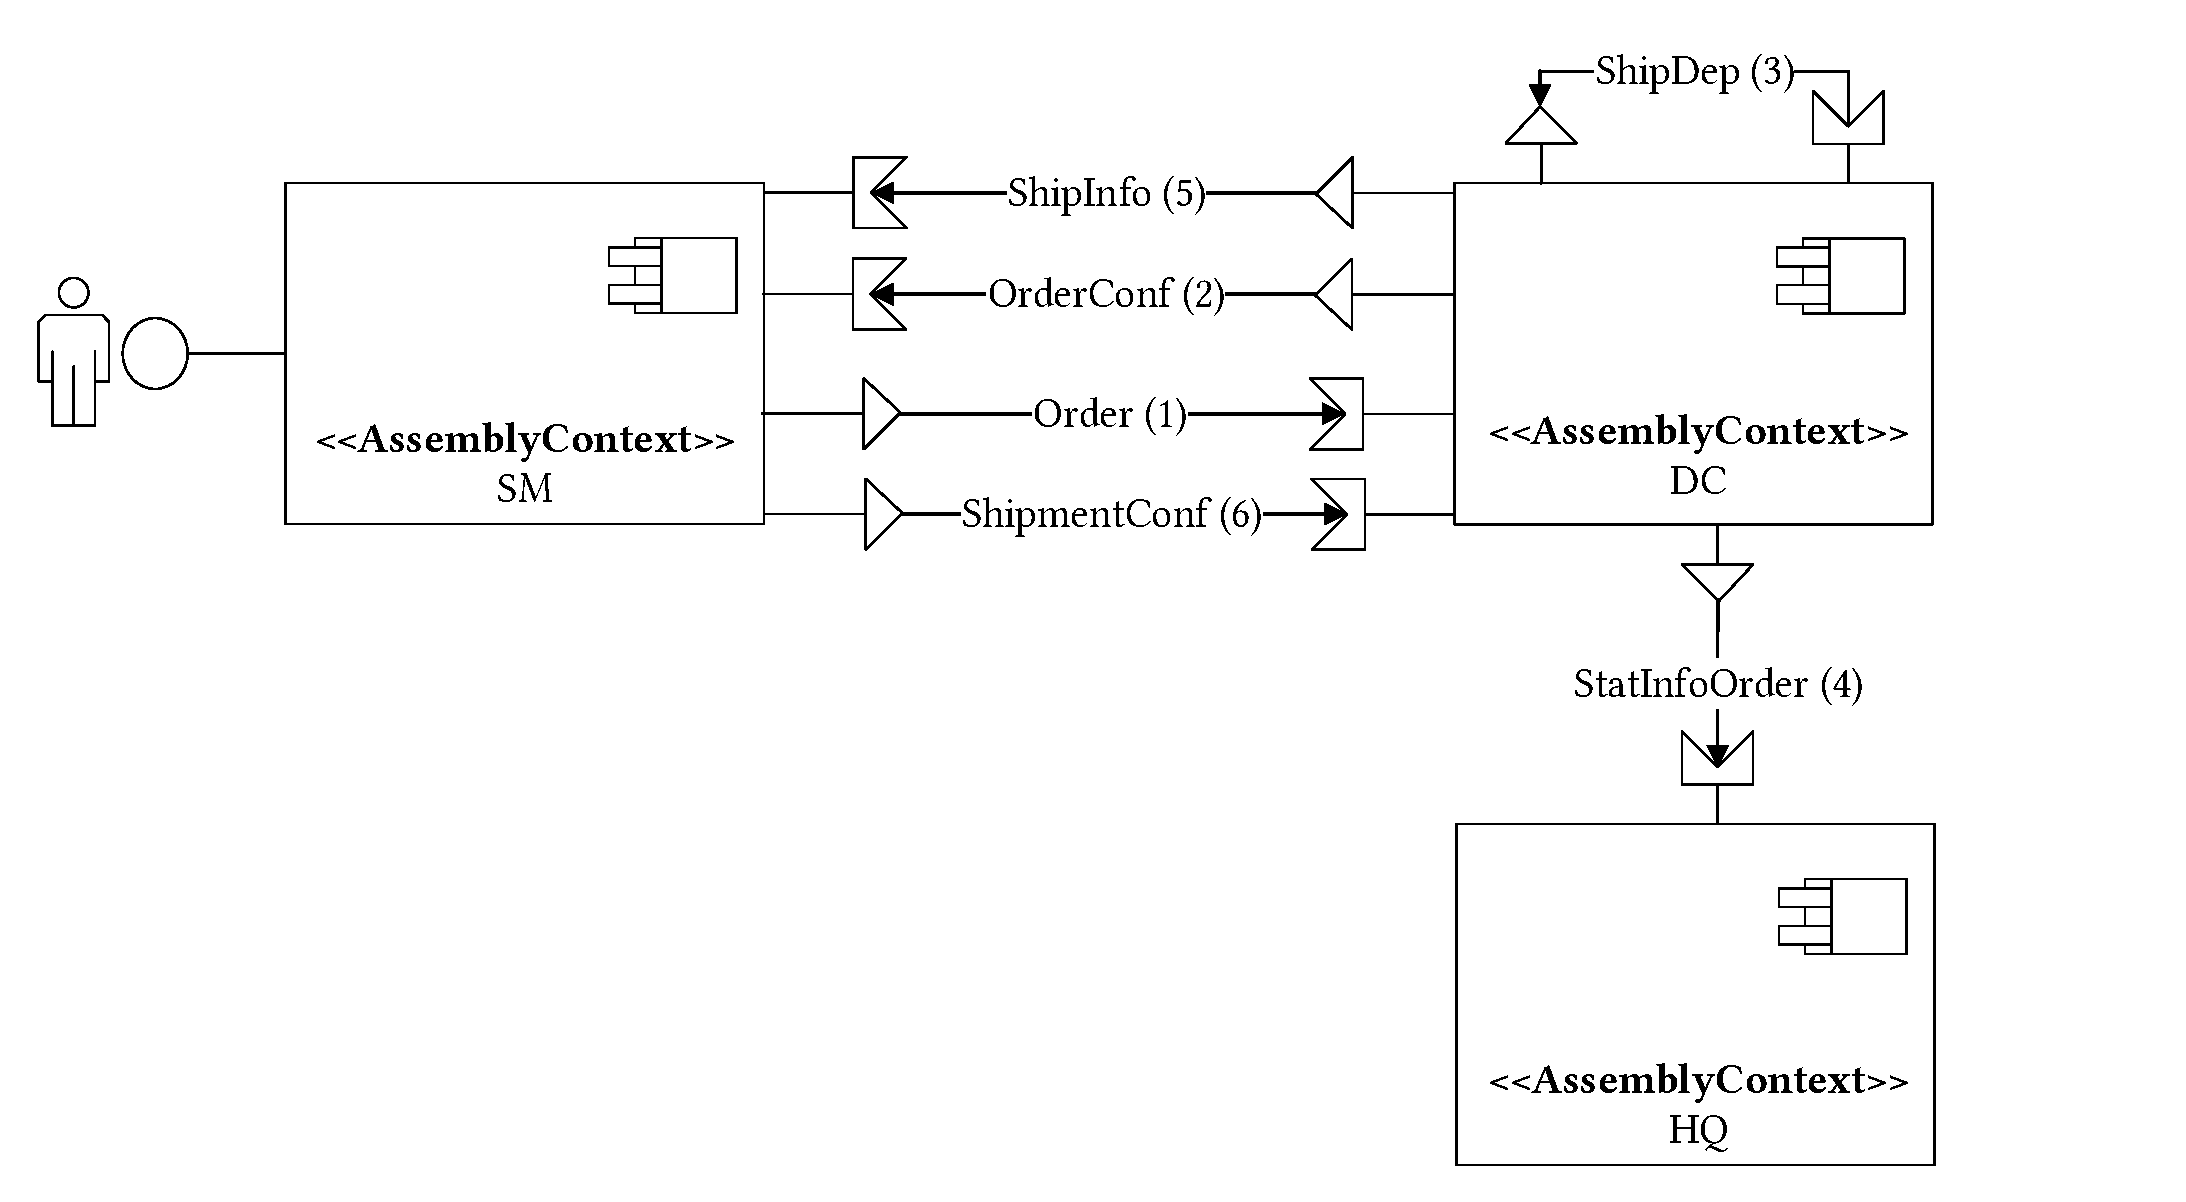
\includegraphics[width=1\textwidth]{images/evaluation/specjms/evaluationInteraktion1events.pdf}
  \caption{Modell der Interaktion 1 des SPECjms2007 mit PCM-Event-Elementen}
  \label{img:interaction1system}
\end{figure}

\begin{figure}
\center
  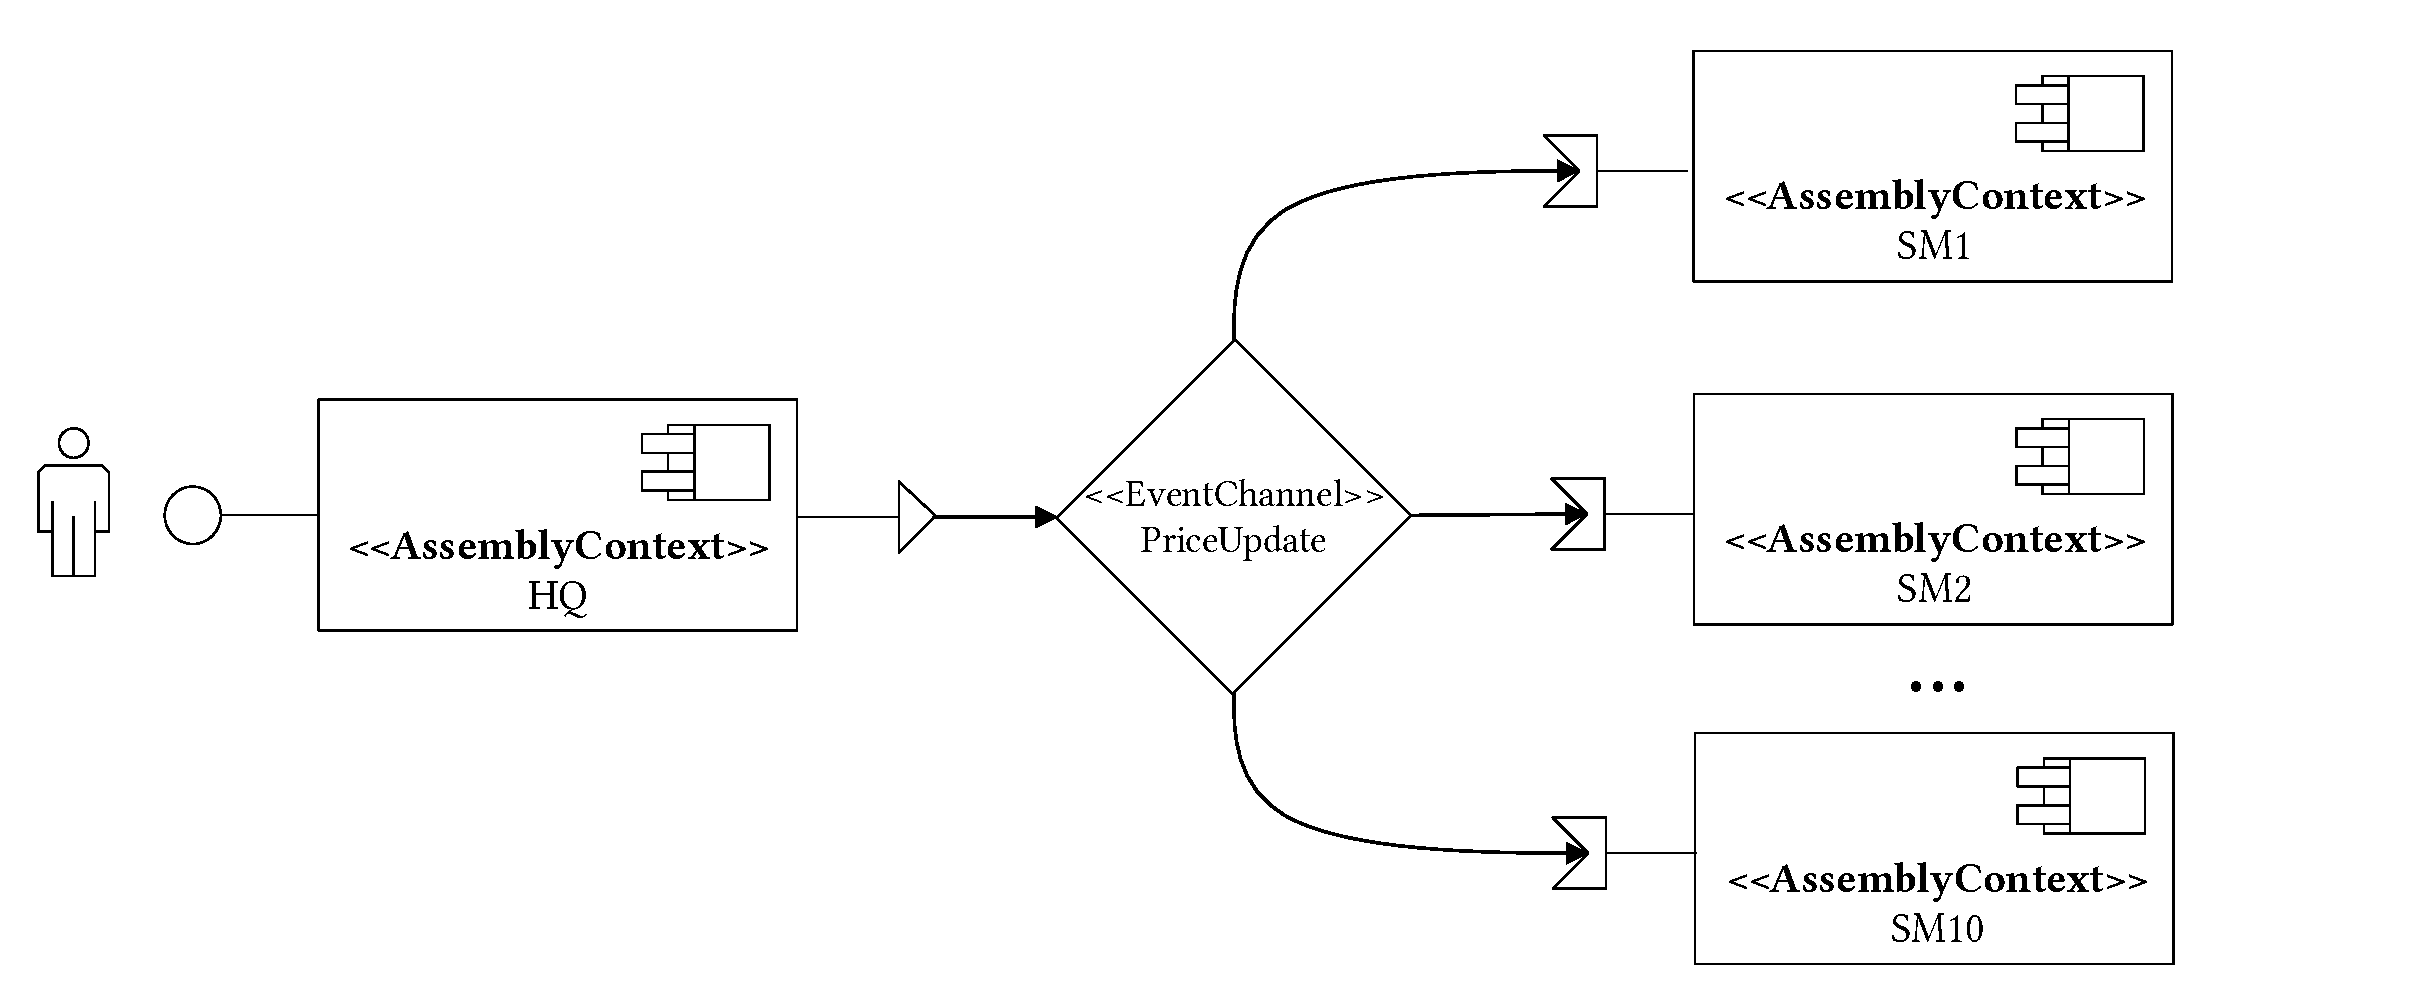
\includegraphics[width=1\textwidth]{images/evaluation/specjms/evaluationInteraktion3events.pdf}
  \caption{Modell der Interaktion 3 des SPECjms2007 mit PCM-Event-Elementen}
  \label{img:interaction3system}
\end{figure}

%\subsection{Ausführungsumgebung und Allokation}

\subsection{Nutzungsmodell}
Das Nutzungsmodell enthält für jede Interaktion ein eigenes UsageScenario. Jedes dieser UsageScenarios beinhaltet einen Aufruf, der im Repository-Modell die jeweilige Interaktion startet. Die Verwendung von separaten UsageScenarios ermöglicht es, für jede Interaktion eine individuelle Senderate festzulegen. Eine Interaktion kann bei Bedarf auch deaktiviert werden. Die Verteilung der verschiedenen Nachrichtengrößen wird an dieser Stelle als Parameterbelegung eingefügt.

\subsection{MOM}
Zusätzlich enthält die Modellierung des SpecJMS ein Middleware-Repository. Dieses besteht aus drei Komponenten die die fünf Middleware-Schnittstellen bereitstellen, damit die Middleware, wie in .. beschrieen, in die Systemarchitektur eingewebt wird. Um die Resourcenanforderung richtig abbilden zu können wurde in der Arbeit von Rathfelder \cite{Rathfelder2013}, für jede Nachricht die Resourcenanforderung ausgemessen. Anschließend wurde das Middleware-Repository-Modell damit kalibriert. Ein Auszug der Resourcenanforderungen für die Nachrichten der Interaktionen eins und drei ist in \autoref{tab:specjmsMsgSizeRd} abgebildet. Um die Ressourcenanforderungen im Middleware-Modell zu spezifizieren wurden  GuardedBranchTransissions verwendet. Dazu wurde zu jedem Nachrichtentyp eine eigene GuardedBranchTransission angelegt, die die Ressourcenanforderung angibt. 

\begin{table}
\center
  \begin{tabular}{|c|l|l|l|l|}
  \hline
    \textbf{Interaktion} & \textbf{Nachricht} & \textbf{CPU-RD 1} & \textbf{CPU-RD 2} &\textbf{CPU-RD 3} \\
    \hline \hline
    \multirow{6}{*}{1} & Order & 0,973 & 0,987 & 1,846 \\\cline{2-5}
    & OrderConf & 0,390 & 0,365 & 0,663 \\\cline{2-5}
    & ShipDep & 0,539 & 1,148 & 2,494\\\cline{2-5}
    & StatInfoOrder & 0,053 & 0,112 & 0,242 \\\cline{2-5}
    & ShipInfo & 0,616 & 1,170 & 2,501 \\\cline{2-5}
    & ShipConf & 0,390 & 0,365 & 0,663  \\\hline
    \hline
     3 & PriceUpdate & 0,501 & 0,501 & 0,501 \\\hline
  \end{tabular}
	\caption{\label{tab:specjmsMsgSizeRd} Ausgerechnete Ressourcenanforderungen für die Nachrichten. Auszug aus \cite{Rathfelder2013}}
\end{table}



\subsection{Anpassung des Modells}
Während in der Arbeit von Rathfelder jede Nachricht des SpecJMS ausgemessen wurde und anschließend über eine Fallunterscheidung in das Middleware-Modell eingesetzt wurde, wurde in dieser Masterarbeit zuerst ein allgemeines System ausgemessen um ein Middleware-Modell zu kalibrieren. Mithilfe dieses Middleware-Modells sollen Vorhersagen über verschiedene System getroffen werden können. Dies ist mit dem Middleware-Repository-Modell aus der Arbeit von Rathfelder nicht möglich, da eine Middleware für ein bestimmtes System ausgemessen wurde. Deshalb wird dieses Middleware-Repository und die darin enthaltene Modellkalibrierung, in der weiteren Evaluierung nicht weiter verwendet und durch den Ansatz aus dieser Masterarbeit ersetzt. 
Die anderen zuvor vorgestellten Modelle werden dagegen wiederverwendet. Außerdem wird eine neue Parameterbelegung für die einzelnen EmitEventActions spezifiziert. Anstelle das die Ressourcenanforderung im Middleware-Modell spezifiziert werden, wird nun die Größe der einzelnen Nachrichten bei der jeweiligen EmitEventAction, mithilfe einer Parameterbelegung, spezifiziert. Eine weitere Anpassung ist, dass die Event-Transformation, die das Middleware-Modell in die Systemarchitektur einwebt nicht verwendet wird. Stattdessen werden die Event-Modell mithilfe der in \autoref{ch:transformation} vorgestellten Modell-Transformation transformiert. Die Ergebnisse der Transformation werden im Folgenden vorgestellt.



%evtl nachrichtengröße wird in usage modell mit angegeben \\


\subsubsection{Interaktion 1}
In \autoref{img:interaction1systemAfterTransformation} ist der Teil des Systemmodells abgebildet, der die Interaktion 1 darstellt. Zu sehen ist, dass die einzelnen Akteure voneinander entkoppelt wurden und an einen zentralen Exchange angeschlossen wurden. Für jeden Nachrichtentyp (EventType) wurde eine Warteschlange angelegt, die ebenfalls an den Exchange angeschlossen wurde. Für die Empfangsaktionen wurde jeweils ein neues UsageScenario angelegt, die jeweils die angeforderte Nachricht, sobald sie in der Warteschlange ist, entnehmen. 
\begin{figure}
\center
  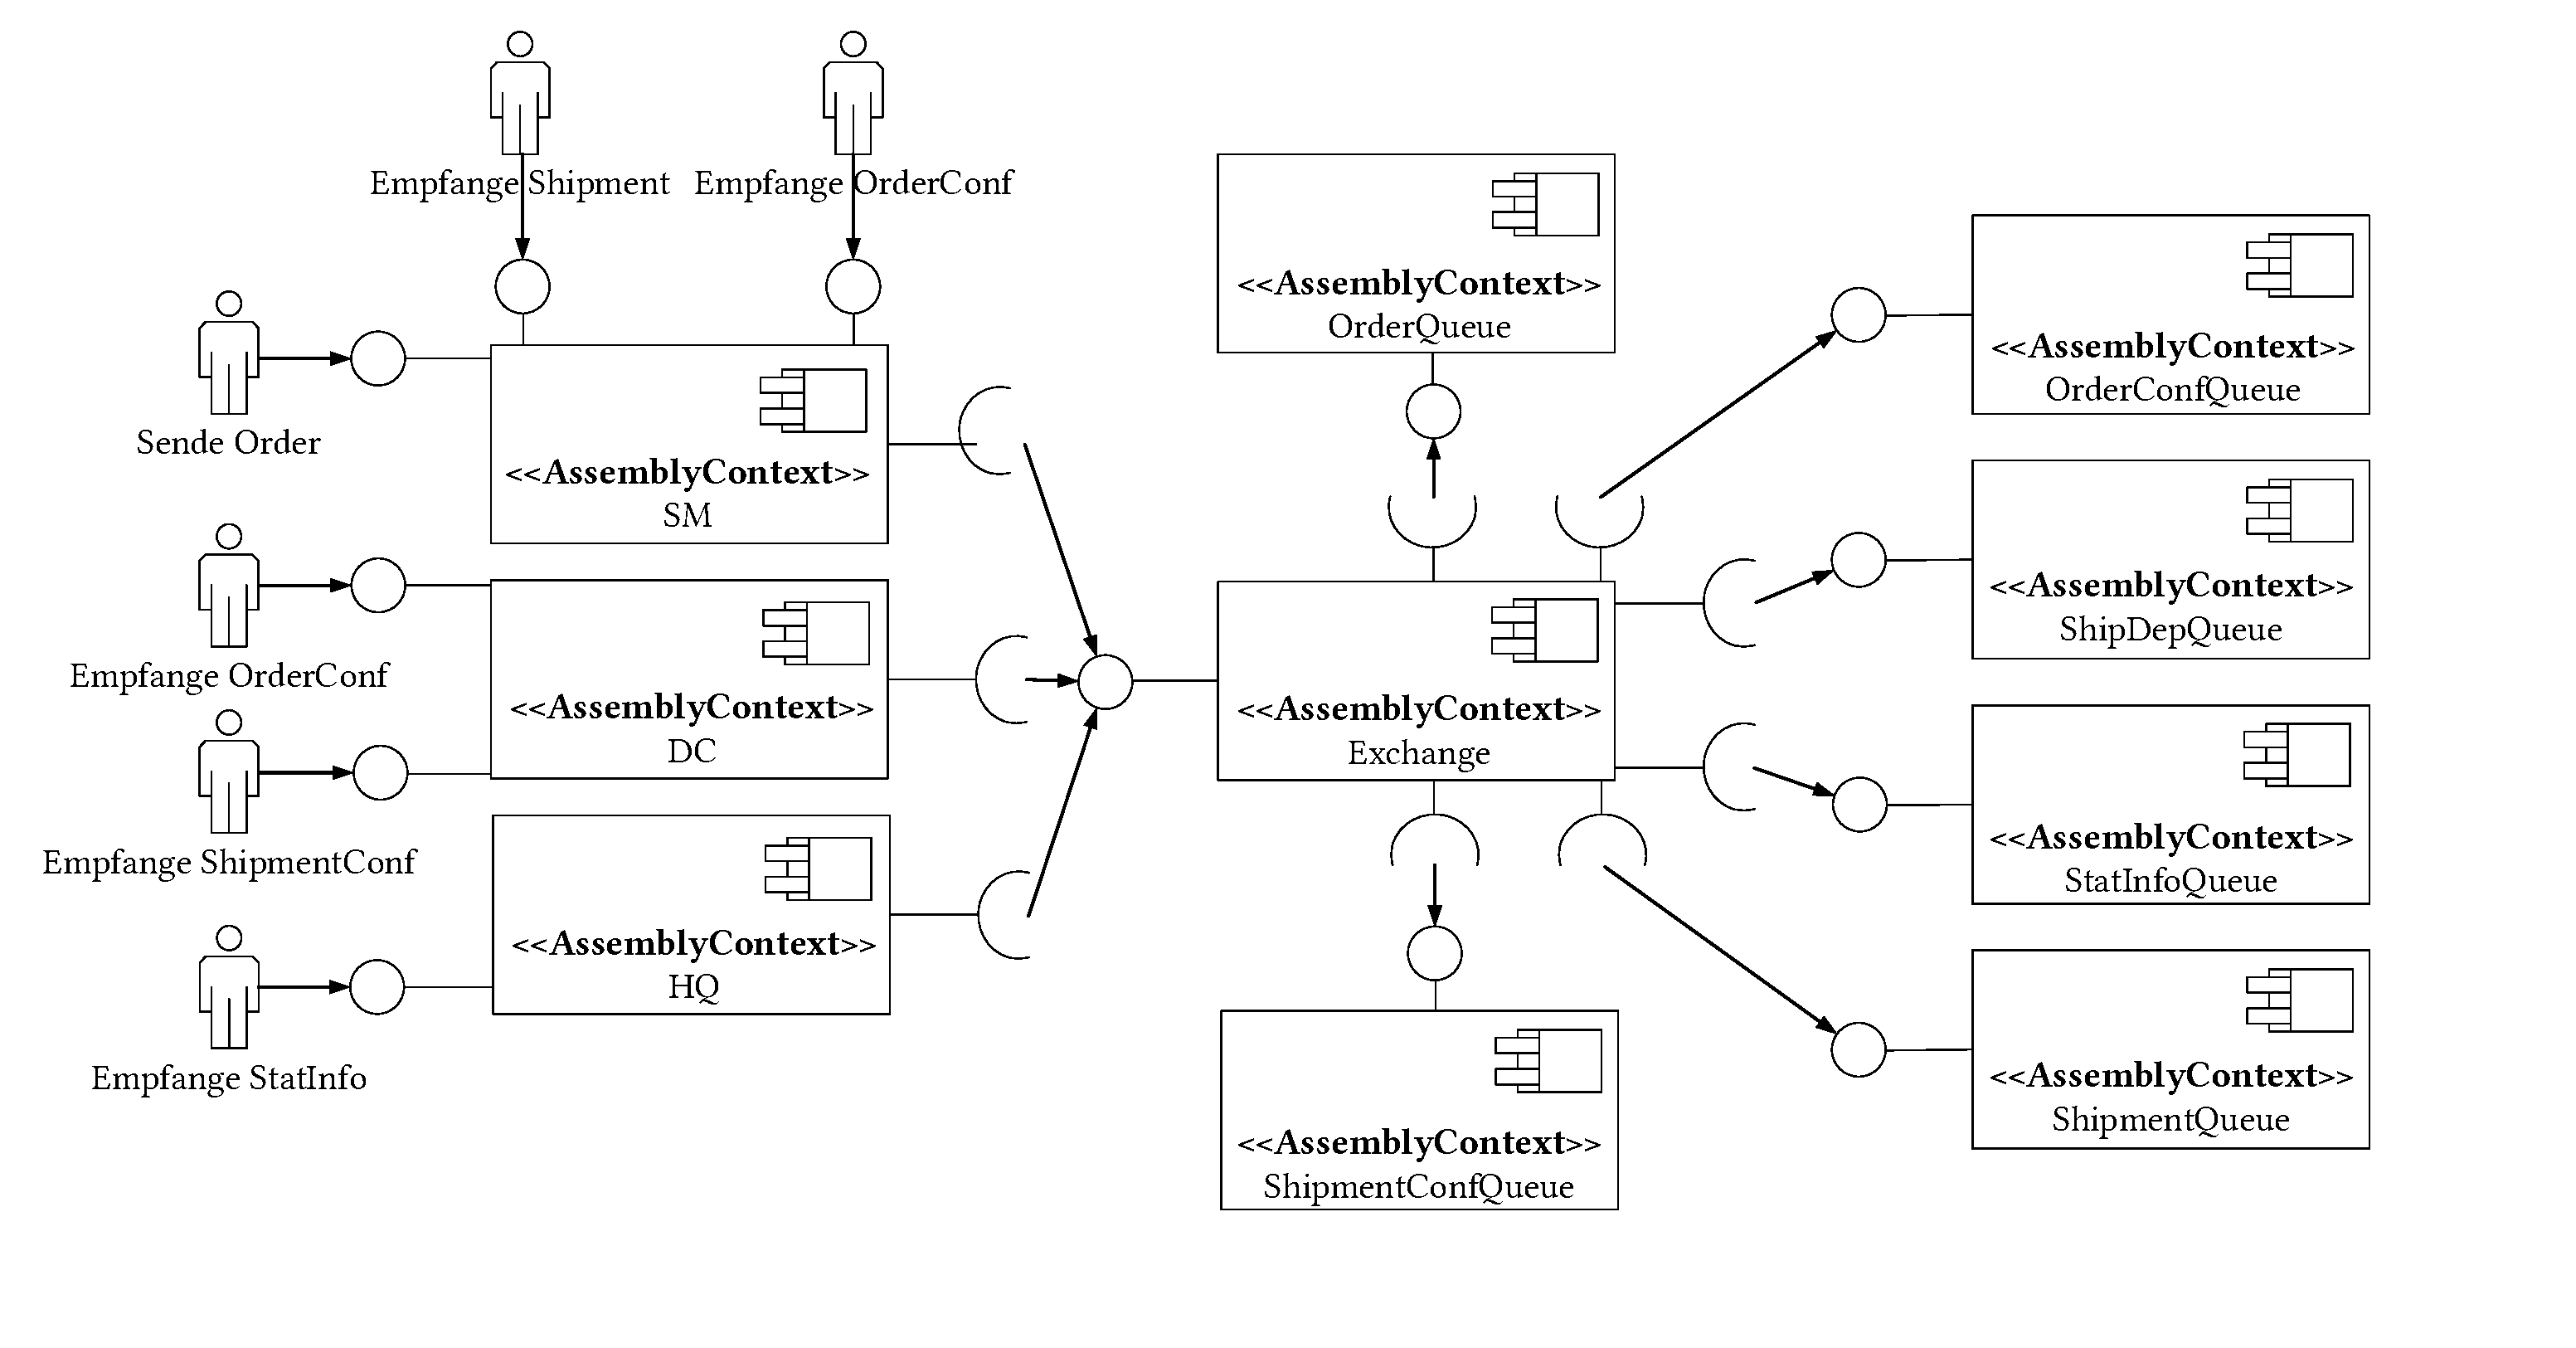
\includegraphics[width=1.4\textwidth,angle=90]{images/evaluation/specjms/evaluationInteraktion1new.pdf}
  \caption{Modell der Interaktion 1 des SPECjms2007 nach der Modelltransformation aus \autoref{ch:transformation}}
  \label{img:interaction1systemAfterTransformation}
\end{figure}
\subsubsection{Interaktion 3}
In \autoref{img:interaction1systemAfterTransformation} ist der Teil des Systemmodells abgebildet, der die Interaktion 3 darstellt. In diesem Fall wurden Empfänger und Sender gemeinsam an den Exchange angeschlossen. Für jeden Empfänger wurde außerdem eine ein Warteschlange angelegt, die ebenfalls an den Exchange angeschlossen wurde. Die einzelnen Warteschlangen beinhalten jeweils den gleichen Nachrichtentyp, hier \emph{PriceUpdate}-Nachrichten. Für die Empfangsaktionen wurde jeweils ein neues \emph{UsageScenario} angelegt, die jeweils die angeforderte Nachricht, sobald sie in der Warteschlange ist, entnehmen.
\autoref{img:interaction3systemAfterTransformation}
\begin{figure}
\center
  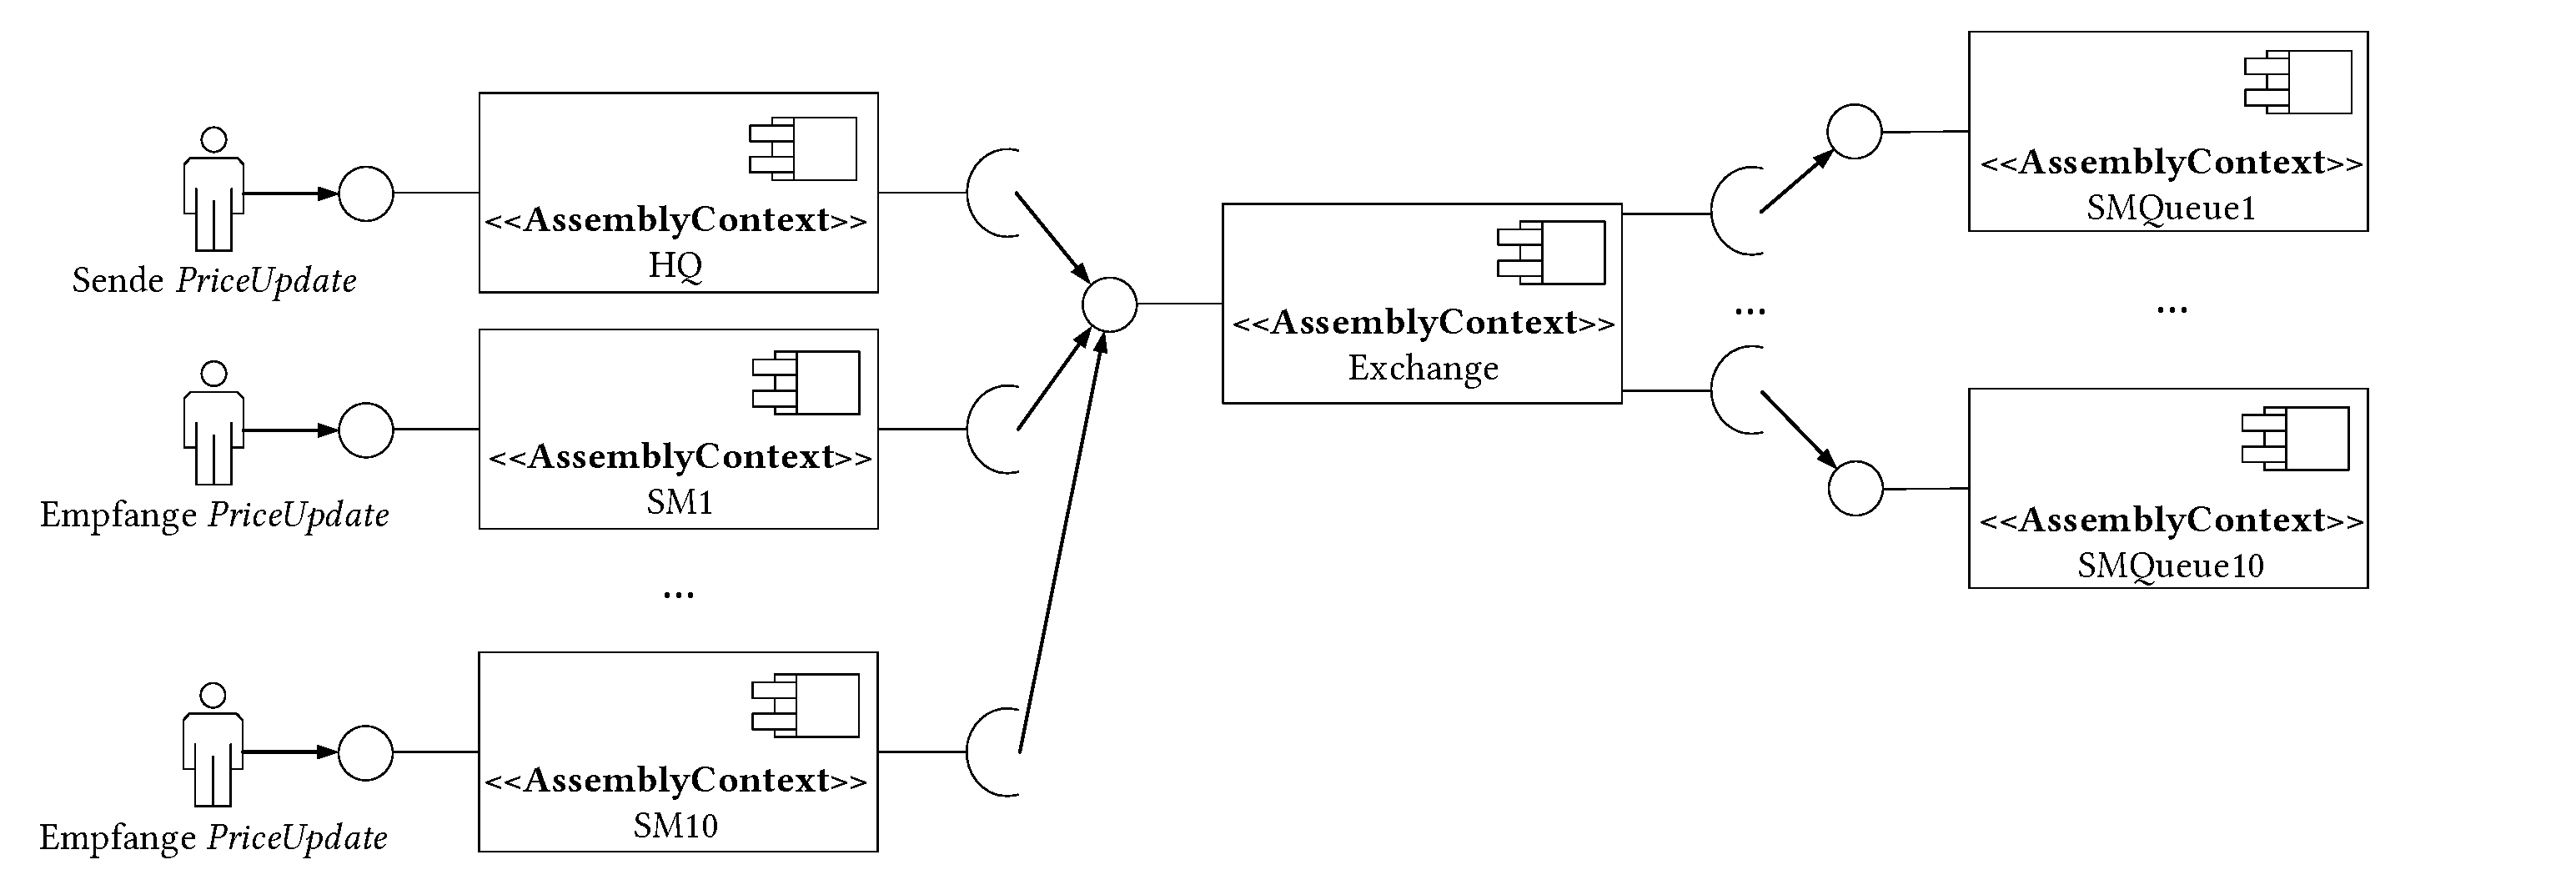
\includegraphics[width=1.4\textwidth,angle=90]{images/evaluation/specjms/evaluationInteraktion3new.pdf}
  \caption{Modell der Interaktion 3 des SPECjms2007 nach der Modelltransformation aus \autoref{ch:transformation}}
  \label{img:interaction3systemAfterTransformation}
\end{figure}


\section{Evaluation der Vorhersagegenauigkeit}
\label{sec:specjmsmodellvorhersage}
Im Folgende soll die Vorhersagegenauigkeit des Ansatzes dieser Masterarbeit mithilfe des zuvor vorgestellten SpecJMS2007-Benchmark und der Modellierung dessen gezeigt werden. Wie bereits erwähnt werden dazu die Interaktionen eins und drei in ihrer, vom Benchmark vorgegebenen, Standard- und einer Lastkonfiguration getestet. Als MOM wurde RMQ verwendet. Die einzelnen Messungen starteten mit eine X sekündigen Aufwärmphase. Im Anschluss wurde eine Y sekündige Messung durchgeführt. Die Dauer wurde aus der Standardkonfiguration des Benchmarks übernommen. Jede Messung wurde zehn mal durchgeführt. Die Experimentumgebung ist, wie schon beim Ausmessen von RMQ, auf einem virtuellen Server ausgeführt worden. Die Spezifikation des Systems ist in \autoref{tab:systespec} abgebildet. Es wurde der Fall betrachtet, dass alle Sender, Empfänger und der RMQ-Broker sich auf der selben Maschine befinden. Somit wurde der Aufbau wie in \autoref{img:machineoverview}a betrachtet. Für die Vorhersage wurde eine Performance-Analyse mithilfe der Palladio-Bench durchgeführt. Als Analysewerkzeug wurde \textbf{SimuCom} verwendet. Im Folgenden werden die Ergebnisse der Messungen und der Vorhersagen aus der Performance-Analyse, für beide Interaktionen und der jeweiligen Konfigurationen, präsentiert. Dazu wird der Fehler zwischen dem gemessenen und vorhergesagten Wert, für die Latenz einer Nachricht, berechnet. Die dazu verwendete Formel ist:
\[ Fehler\% = \frac{|Vorhersage - Messung|}{Messung} * 100 \]
Der SpecJMS Benchmark liefert für jede Interaktion eine Interaktionszeit, die angibt, wie lange die Interaktion vom Senden der ersten Nachricht, bis zum Empfangen der letzten Nachricht gedauert hat. Außerdem wird für jede Nachricht die gesendet wird, auch die Latenz geliefert. Bei der Präsentation der Ergebnisse werden beide Werte verglichen. Die Performance-Analyse liefert hingegen nur die Latenz der einzelnen Nachrichten. Um eine Annäherung an die Interaktionszeit zu bekommen, werden die jeweils relevanten Ergebnisse aufaddiert.
%CPU Auslastung des Specjms vs. Modellierung\\
%mehrer Messungen für Interaktion => Boxplot, der einen Median zeigt. Mit diesem wird dann das Modell verglichen.
\subsection{Interaktion 1}
Die Messergebnisse für Interaktion 1 des SPECjms2007 Benchmarks und der Performance-Analyse des Modells, sind in  \autoref{img:specjminteraction1results} abgebildet. Dabei sind für jede Nachricht die jeweiligen Messergebnisse, der Durchschnittslatenz, eingezeichnet. Außerdem wurde für jede Nachricht der Median eingezeichnet. Die Vorhersage durch die Performance-Analyse wurde auch eingetragen. In \autoref{tab:interaction1error} sind die Fehler für die jeweilige Nachricht eingetragen. Dabei ist zu sehen, dass dieser zwischen 20,76\% und 23,79\% liegt. 

\begin{figure}
\center
  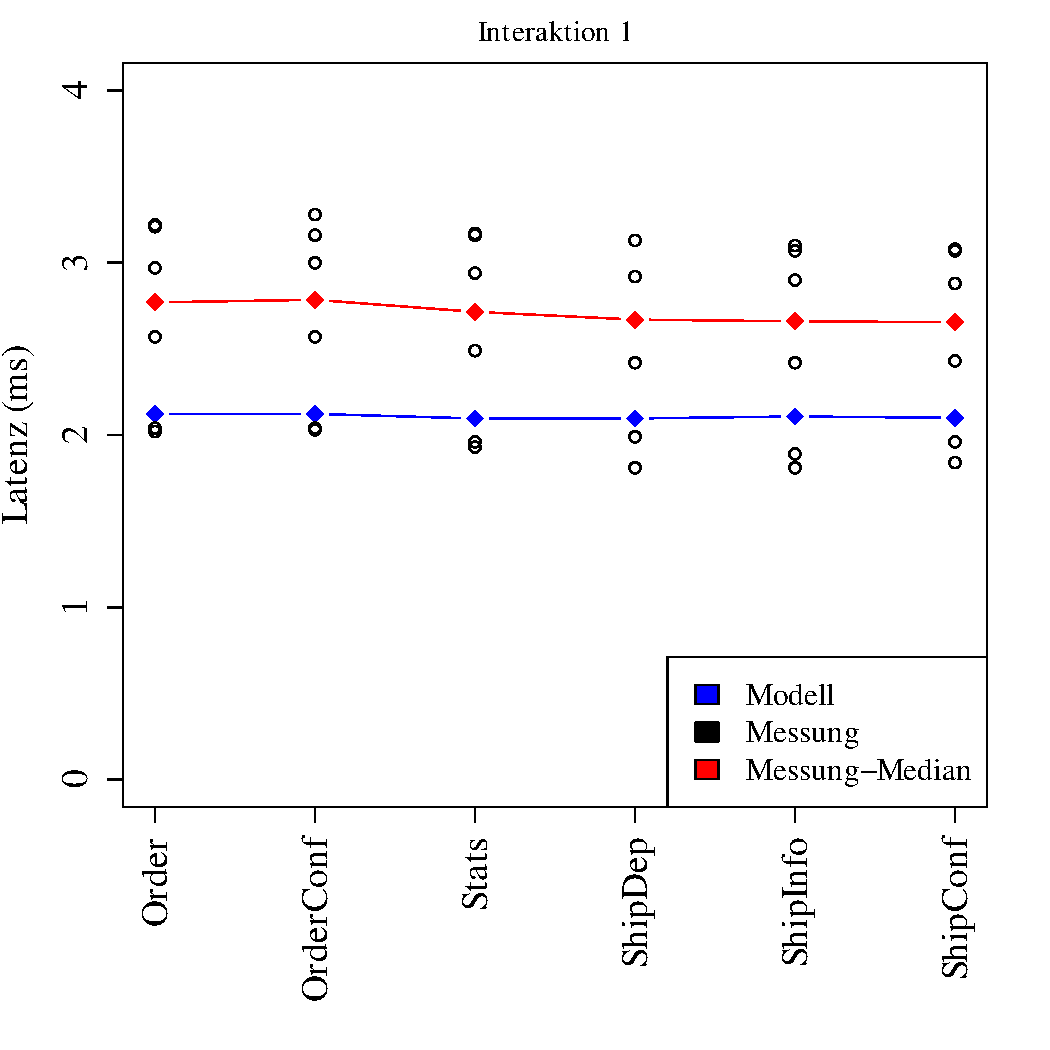
\includegraphics[width=0.6\textwidth]{images/evaluation/specjmsresults/interaktion1.pdf}
  \caption{Latenz der Messung und Vorhersage für die Nachrichten aus Interaktion 1 des SPECjms2007 Benchmark}
  \label{img:specjminteraction1results}
\end{figure}

In \autoref{img:specjminteraction1interactiontimeresults} ist außerdem ein Boxplot für die gesamte Interaktionszeit abgebildet. Diese setzt sich aus der Latenz der einzelnen Nachrichten wie folgt zusammen: \[Order + max(OrderConf, ShipDep, StatInfoOrder) + ShipInfo + ShipConf\] 
Die Vorhersage der Interaktionszeit aus der Performance-Analyse ist 8,43 ms. Der Fehler zwischen dem Median der gemessenen Interaktionszeit und der Vorhersage beträgt 6,37\%.
%noch mit groesseren Nachrichten \\

\begin{figure}
\center
  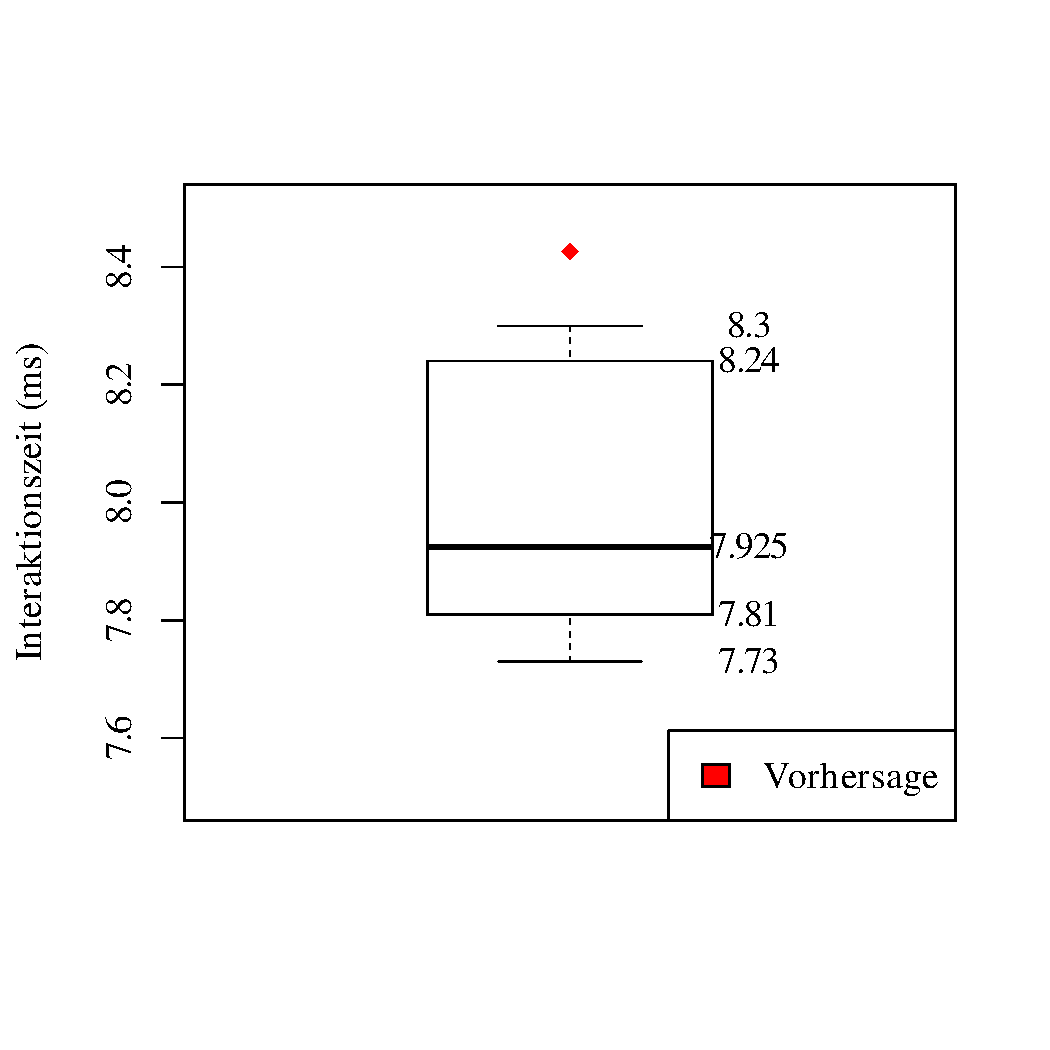
\includegraphics[width=0.6\textwidth]{images/evaluation/specjmsresults/interaktion1InteractionTime.pdf}
  \caption{Boxplot von zehn verschiedenen Messungen von Interaktion 1 des SPECjms2007 Benchmark}
  \label{img:specjminteraction1interactiontimeresults}
\end{figure}

%\subsubsection{Msg Rate 1}
%Für diesen Vergleich wurde die Senderate der Bestellungen auf eine Bestellung die Sekunde limitiert. Im Anschluss wurde die Interaktion gestartet und nach 10 Minuten beendet. Diese Messung wurde 10 mal durchgeführt. Die durchschnittlichen Interaktionszeiten sind in \autoref{img:specjmsMsgRate1Impl} als Boxplot dargestellt. TODO Boxplot beschreiben. Die Simulation der Modellierung liefert eine Interaktionszeit von 9500 Mikrosekunden (Mit Bild?). Die Fehler sind in \autoref{tab:interaction1msgrate1error} abgebildet. Somit liegt der Fehler fuer diesen Vergleich zwischen 24.66\% und 31.21\%. 

\begin{table}
  \begin{tabular}{|l|c|c|c|c|c|c|}
  \hline
    Nachricht & Order & OrderConf & ShipDep & StatInfo & ShipInfo & ShipConf \\
    \hline
    Messung (ms) & 2,77 & 2,785 & 2,67 & 2,715 & 2,66 & 2,655 \\\hline
    Vorhersage (ms) & 2,12 & 2,12 & 2,1 & 2,1 & 2,11 & 2,1 \\\hline
    Fehler (\%)& 23,36 & 23,79 & 21,5 & 22,8 & 20,76 & 20,91 \\\hline
  \end{tabular}
	\caption{\label{tab:interaction1error} Übersicht der Fehler für Interaktion 1 des SPECjms2007 Benchmark}
\end{table}

\subsection{Interaktion 3}
In \autoref{img:specjminteraction3results10sm} ist ein Boxplot für die Messungen der Interaktion 3 des SPECjms2007 Benchmark eingezeichnet. Der Median der Latenz, der \emph{PriceUpdate}-Nachricht, beträgt 4,3ms. Die Performance-Analyse liefert eine Latenz von 2,1ms. Der Fehler liegt somit bei 51,16\% und ist somit höher als 40\%, was der in Literatur akzeptierte Wert ist.

\begin{figure}
\center
  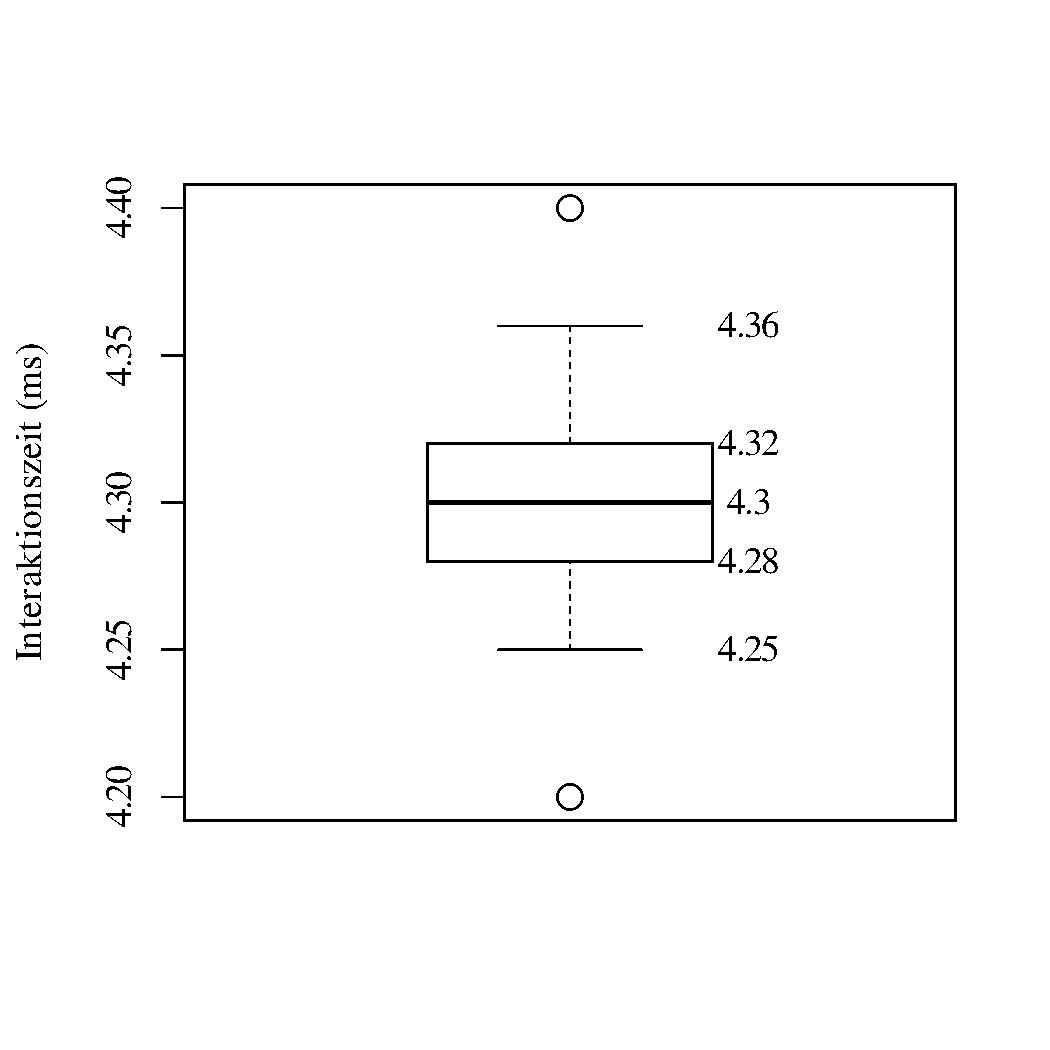
\includegraphics[width=0.6\textwidth]{images/evaluation/specjmsresults/interaktion3-10SM.pdf}
  \caption{Boxplot von zehn verschiedenen Messungen von Interaktion 3 mit zehn Empfängern}
  \label{img:specjminteraction3results10sm}
\end{figure}

In \autoref{img:specjminteraction3results1sm} wurde der Benchmark nochmal ausgeführt, jedoch mit einem SM anstatt zehn SMs. Der Median der Latenz beträgt in diesem Fall 2,84ms. Die Performance-Analyse liefert wieder eine Latenz von 2,1ms. Der Fehler liegt nun bei 26,06\%. Dies liegt wahrscheinlich daran, dass beim Senden einer Publish/Subscribe-Nachricht eine nicht beachtete Ressourcenanforderung stattfindet.
\begin{figure}
\center
  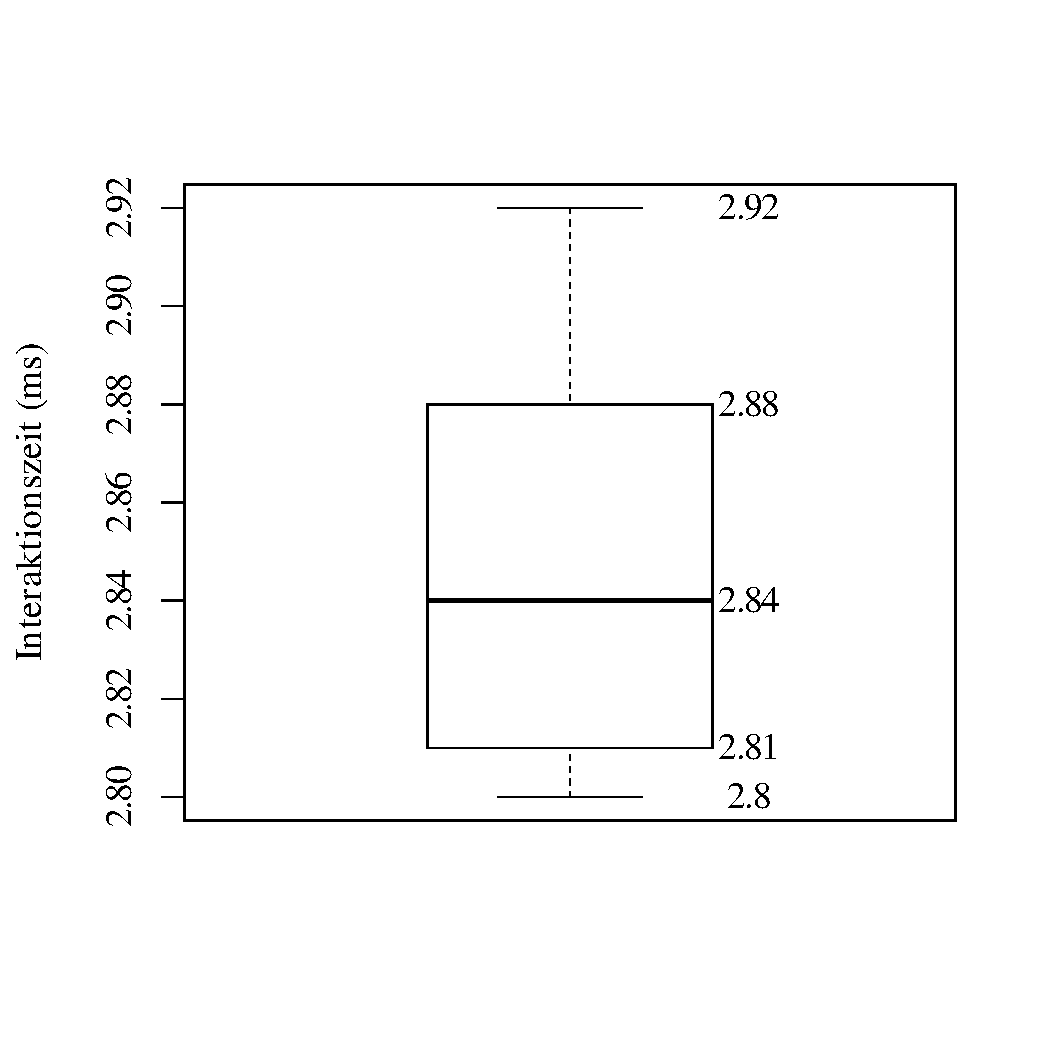
\includegraphics[width=0.6\textwidth]{images/evaluation/specjmsresults/interaktion3-1SM.pdf}
  \caption{Boxplot von zehn verschiedenen Messungen von Interaktion 3 mit einem Empfänger}
  \label{img:specjminteraction3results1sm}
\end{figure}


\section{Zusammenfassung der Evaluation}
\label{sec:evaluationzusammenfassung}
In diesem Kapitel wurde der Ansatz dieser Masterarbeit mithilfe des SPECjms2007 Benchmark evaluiert. In \autoref{tab:gqm} wurden dazu die Ziele der Evaluierung mithilfe des GQM-Plans formuliert. Im Folgenden wird darauf eingegangen, ob und wie diese Ziele erreicht werden konnten. \par
In \autoref{sec:specjmsmodell} wurden die PCM-Modelle, die den Benchmark modellieren, vorgestellt. Im Anschluss wurden sie mithilfe der Modeltransformation aus \autoref{ch:transformation} transformiert. Dabei konnte gezeigt werden, dass die in \autoref{ch:modellierung} vorgestellte Art eine MOM zu modellieren anwendbar ist. Somit konnte das erste Ziel dieser Arbeit erfüllt werden. 
In \autoref{sec:specjmsmodellvorhersage} wurde die Vorhersagegenauigkeit der Modellierung und ihrer Kalibrierung geprüft. Diese hat gezeigt, dass dies bei einer Punkt-Zu-Punkt-Kommunikation möglich ist, da der Fehler der einzelnen Nachrichten unter 24\% und für die Gesamte Interaktion unter 7\% liegt. Die Vorhersagegenauigkeit für Publish/Subscribe-Kommunikation konnte, mit der aktuellen Kalibrierung, nicht gezeigt werden. Der Fehler beträgt über 40\% und ist somit nicht mehr akzeptiert. Dies zeigt, dass die aktuelle Kalibrierung Publish/Subscribe-Kommunikation nicht unterstützt. Somit konnte das zweite Ziel nur zur Hälfte erreicht werden. \par
In der Arbeit von Rathfelder \cite{Rathfelder2013} liegt der Fehler zwischen 20\% und 25\%. Somit bietet der Ansatz dieser Masterarbeit eine ähnlichen Vorhersagegenauigkeit an.

%Modellierungsaufwand \\

%Modellierung eroeffnet neue moeglichkeiten\\

%\section{TIME}
%Ein weiteres System, das die Anforderungen aus \autoref{sec:systemanforderungen} erfüllt, ist das Transport Information Monitoring Environment (TIME) System \cite{time}. Dabei handelt es sich um ein System der Universität Cambridge. TIME soll ein reales Verkehrsüberwachungssystem darstellen. Es besteht aus mehreren verteilten Komponenten, die verschiedene Arten von Ereignissen senden bzw. empfangen. Die standardmäßige Middleware hat eine Peer-To-Peer Architektur, Punkt-zu-Punkt Kommunikation und unterstützt asynchronen Nachrichtenaustausch. Das System überwacht Autos mithilfe von Kennzeichenerkennung und soll den Verkehrsfluss optimieren. Diese Anwendung ist interessant, weil sie Daten von verschiedenen verteilten Sensoren und Systemen sammelt und integriert. Darüber hinaus enthält es Komponenten mit hohem und unterschiedlichem Ressourcenbedarf, wie z.B. der Kennzeichenerkennungsalgorithmus. Die Systemarchitektur ist sehr anpassungsfähig, wenn es darum geht, neue Komponenten hinzuzufügen oder die Verbindungen zwischen Komponenten oder deren Standort zu ändern. Was dazu führt, dass das hinzufügen und austauschen von verschiedenen MOMs möglich ist. Für die Masterarbeit liegt sowohl die Implementierung, als auch eine PCM-Modellierung des TIME Systems aus einer früheren Arbeit von Christoph Rathfelder \cite{Rathfelder2013} vor. Das TIME System soll für diese Masterarbeit als Evaluierungssystem dienen. Die Modellierung/Implementierung soll zunächst als Referenz für die Performanzanalyse dienen und im nächsten Schritt um verschiedene MOMs erweitert werden.
%% LaTeX2e class for student theses
%% sections/evaluation.tex
%% 
%% Karlsruhe Institute of Technology
%% Institute for Program Structures and Data Organization
%% Chair for Software Design and Quality (SDQ)
%%
%% Dr.-Ing. Erik Burger
%% burger@kit.edu
%%
%% Version 1.3.3, 2018-04-17

\chapter{Zusammenfassung}
\label{ch:zusammenfassung}


%1. Zusammenfassung: Was wurde in dieser Arbeit gemacht? Was waren die Schlüsselergebnisse? Diesmal jedoch zusammengefasst nochmals für einen Leser, der die vorherigen Seiten mit allen Details bereits gelesen hat.
Prozess um MOM auszumessen, modellieren, kalibrieren, transformieren und evaluieren.
%2. Adressaten der Verbesserung: Wem nützen die Verbesserungen/Beiträge der Arbeit? Inwieweit wird die Software-Technik durch die Arbeit verbessert?
Softwarearchitekt kann Auswirkung einer MOM an seiner Software-Architektur sehen. 
%3. Aufbauende/Zukünftige Arbeiten: Welche nächsten Schritte sind geplant (erst kurzfristige, dann längerfristige)? Welche möglichen Lösungsansätze für noch bestehende Probleme sind denkbar? Wie könnten Folgearbeiten aussehen?
Ausblick\\
Nachrichtenanzahl und Nachrichtengröße betrachten bei der Ausmessung \\
Messe Zeit von Sendenr und Empfänger getrennt und pflege es in Modell ein, momentan ist alles in Sender eingetragen \\
weitere effekte \\
batching \\
wartschlange als tatsächliches PCM Element nicht über passive Ressource (kann nachricht durch system tracken)

%% --------------------
%% |   Bibliography   |
%% --------------------

%% Add entry to the table of contents for the bibliography

\printbibliography[heading=bibintoc]

%% ----------------
%% |   Appendix   |
%% ----------------
%\appendix
%%% LaTeX2e class for student theses
%% sections/apendix.tex
%% 
%% Karlsruhe Institute of Technology
%% Institute for Program Structures and Data Organization
%% Chair for Software Design and Quality (SDQ)
%%
%% Dr.-Ing. Erik Burger
%% burger@kit.edu
%%
%% Version 1.3.3, 2018-04-17

\iflanguage{english}
{\chapter{Appendix}}    % english style
{\chapter{Anhang}}      % german style
\label{chap:appendix}


%% -------------------
%% | Example content |
%% -------------------
\section{First Appendix Section}
\label{sec:appendix:FirstSection}
		
\setcounter{figure}{0}
		
\begin{figure} [ht]
  \centering
  \caption{A figure}
  \label{fig:anotherfigure}
\end{figure}


\dots
%% ---------------------
%% | / Example content |
%% ---------------------

\end{document}
